\documentclass[11pt, oneside]{article}   	% use "amsart" instead of "article" for AMSLaTeX format
\usepackage{geometry}                		% See geometry.pdf to learn the layout options. There are lots.
\geometry{a4paper}
%\addtolength{\hoffset}{2cm}
%\addtolength{\marginparwidth}{2cm}
                   		% ... or a4paper or a5paper or ... 
%\geometry{landscape}                		% Activate for for rotated page geometry
%\usepackage[parfill]{parskip}    		% Activate to begin paragraphs with an empty line rather than an indent
\usepackage{graphicx}				% Use pdf, png, jpg, or eps§ with pdflatex; use eps in DVI mode
								% TeX will automatically convert eps --> pdf in pdflatex		
\usepackage{amssymb}
\usepackage{amsmath}
\usepackage[version=3]{mhchem}
\usepackage{rotating}
\usepackage{hyperref}
\usepackage{float}
\usepackage{verbatimbox}
%\usepackage[obeyspaces,spaces]{url}
\usepackage{textcomp}
\usepackage{color}
\usepackage[normalem]{ulem}
\usepackage[obeyDraft, obeyFinal, textsize=scriptsize]{todonotes}
\usepackage{multirow}
\usepackage{enumitem}
\reversemarginpar

\title{Fitting MD torsional terms to QM torsional profiles}
\author{Ivan Welsh}
%\date{}							% Activate to display a given date or no date

\floatstyle{plain}
\newfloat{example}{thp}{exp}
\floatname{example}{Example}

\setcounter{secnumdepth}{2}

\newcommand{\done}[1]{\todo[backgroundcolor=blue!30, linecolor=blue]{#1}}
\newcommand{\todiscuss}[1]{\todo[backgroundcolor=red!50, linecolor=red]{#1}}
\newcommand{\finished}[1]{\todo[backgroundcolor=green!60, linecolor=green]{#1}}

\begin{document}
\maketitle

The ultimate goal of this work is to determine torsional parameters for a molecular mechanics (MM) force field for use in molecular dynamics (MD) simulations based on rotational energy profiles derived from quantum mechanical (QM) calculations, and to determine how generalisable the MD torsional terms are. The former is done by comparing the dihedral rotational energy profile computed using a MM force field without a dihedral term to the QM dihedral rotational energy profile, and fitting a finite series of cosine terms to the resulting energy difference profile. In order to achieve the latter, as well as to minimise the size and number of systems that need to be subjected to QM calculations, it is necessary to first determine the bonded distance required between a dihedral of interest and a functional group such that the functional group has minimal effect on the dihedral rotation profile.\\

\section{Procedure Overview}

A set of twenty, simple organic molecules were chosen for this investigation (Figure~\ref{fig:structures}). The molecules differ only in terms of the nature of the functional group, and how many bonds separate that group from the dihedral angle of interest.\\
The reference QM dihedral rotation energy profiles were determined by carrying out a series of QM calculations where the dihedral of interest ($\psi$ in figure~\ref{fig:structures}) has been fixed at a given value, for a range of $\psi$ values. At each fixed $\psi$ value, the structure of the remainder of the molecule was optimised. The differences in energy across these $\psi$ values (relative to the highest energy state) give the dihedral rotational profile. 
%\begin{sidewaysfigure}[p]
%\centering
%\includegraphics[width=0.9\textheight]{Images/molecules}
%\caption{Chemical structures of the molecules for which torsional profiles were attained.}
%\todo[inline]{Need to add the -1 row}
%\label{fig:structures}
%\end{sidewaysfigure}
\begin{sidewaysfigure}
\centering
\resizebox{\textwidth}{!}{%
\begin{tabular}{|c|c|c|c|c|c|}
\hline
 & AMINO & CHLORO & HYDRO & METH & THIO \\ \hline
\multirow{2}{*}{-1} & 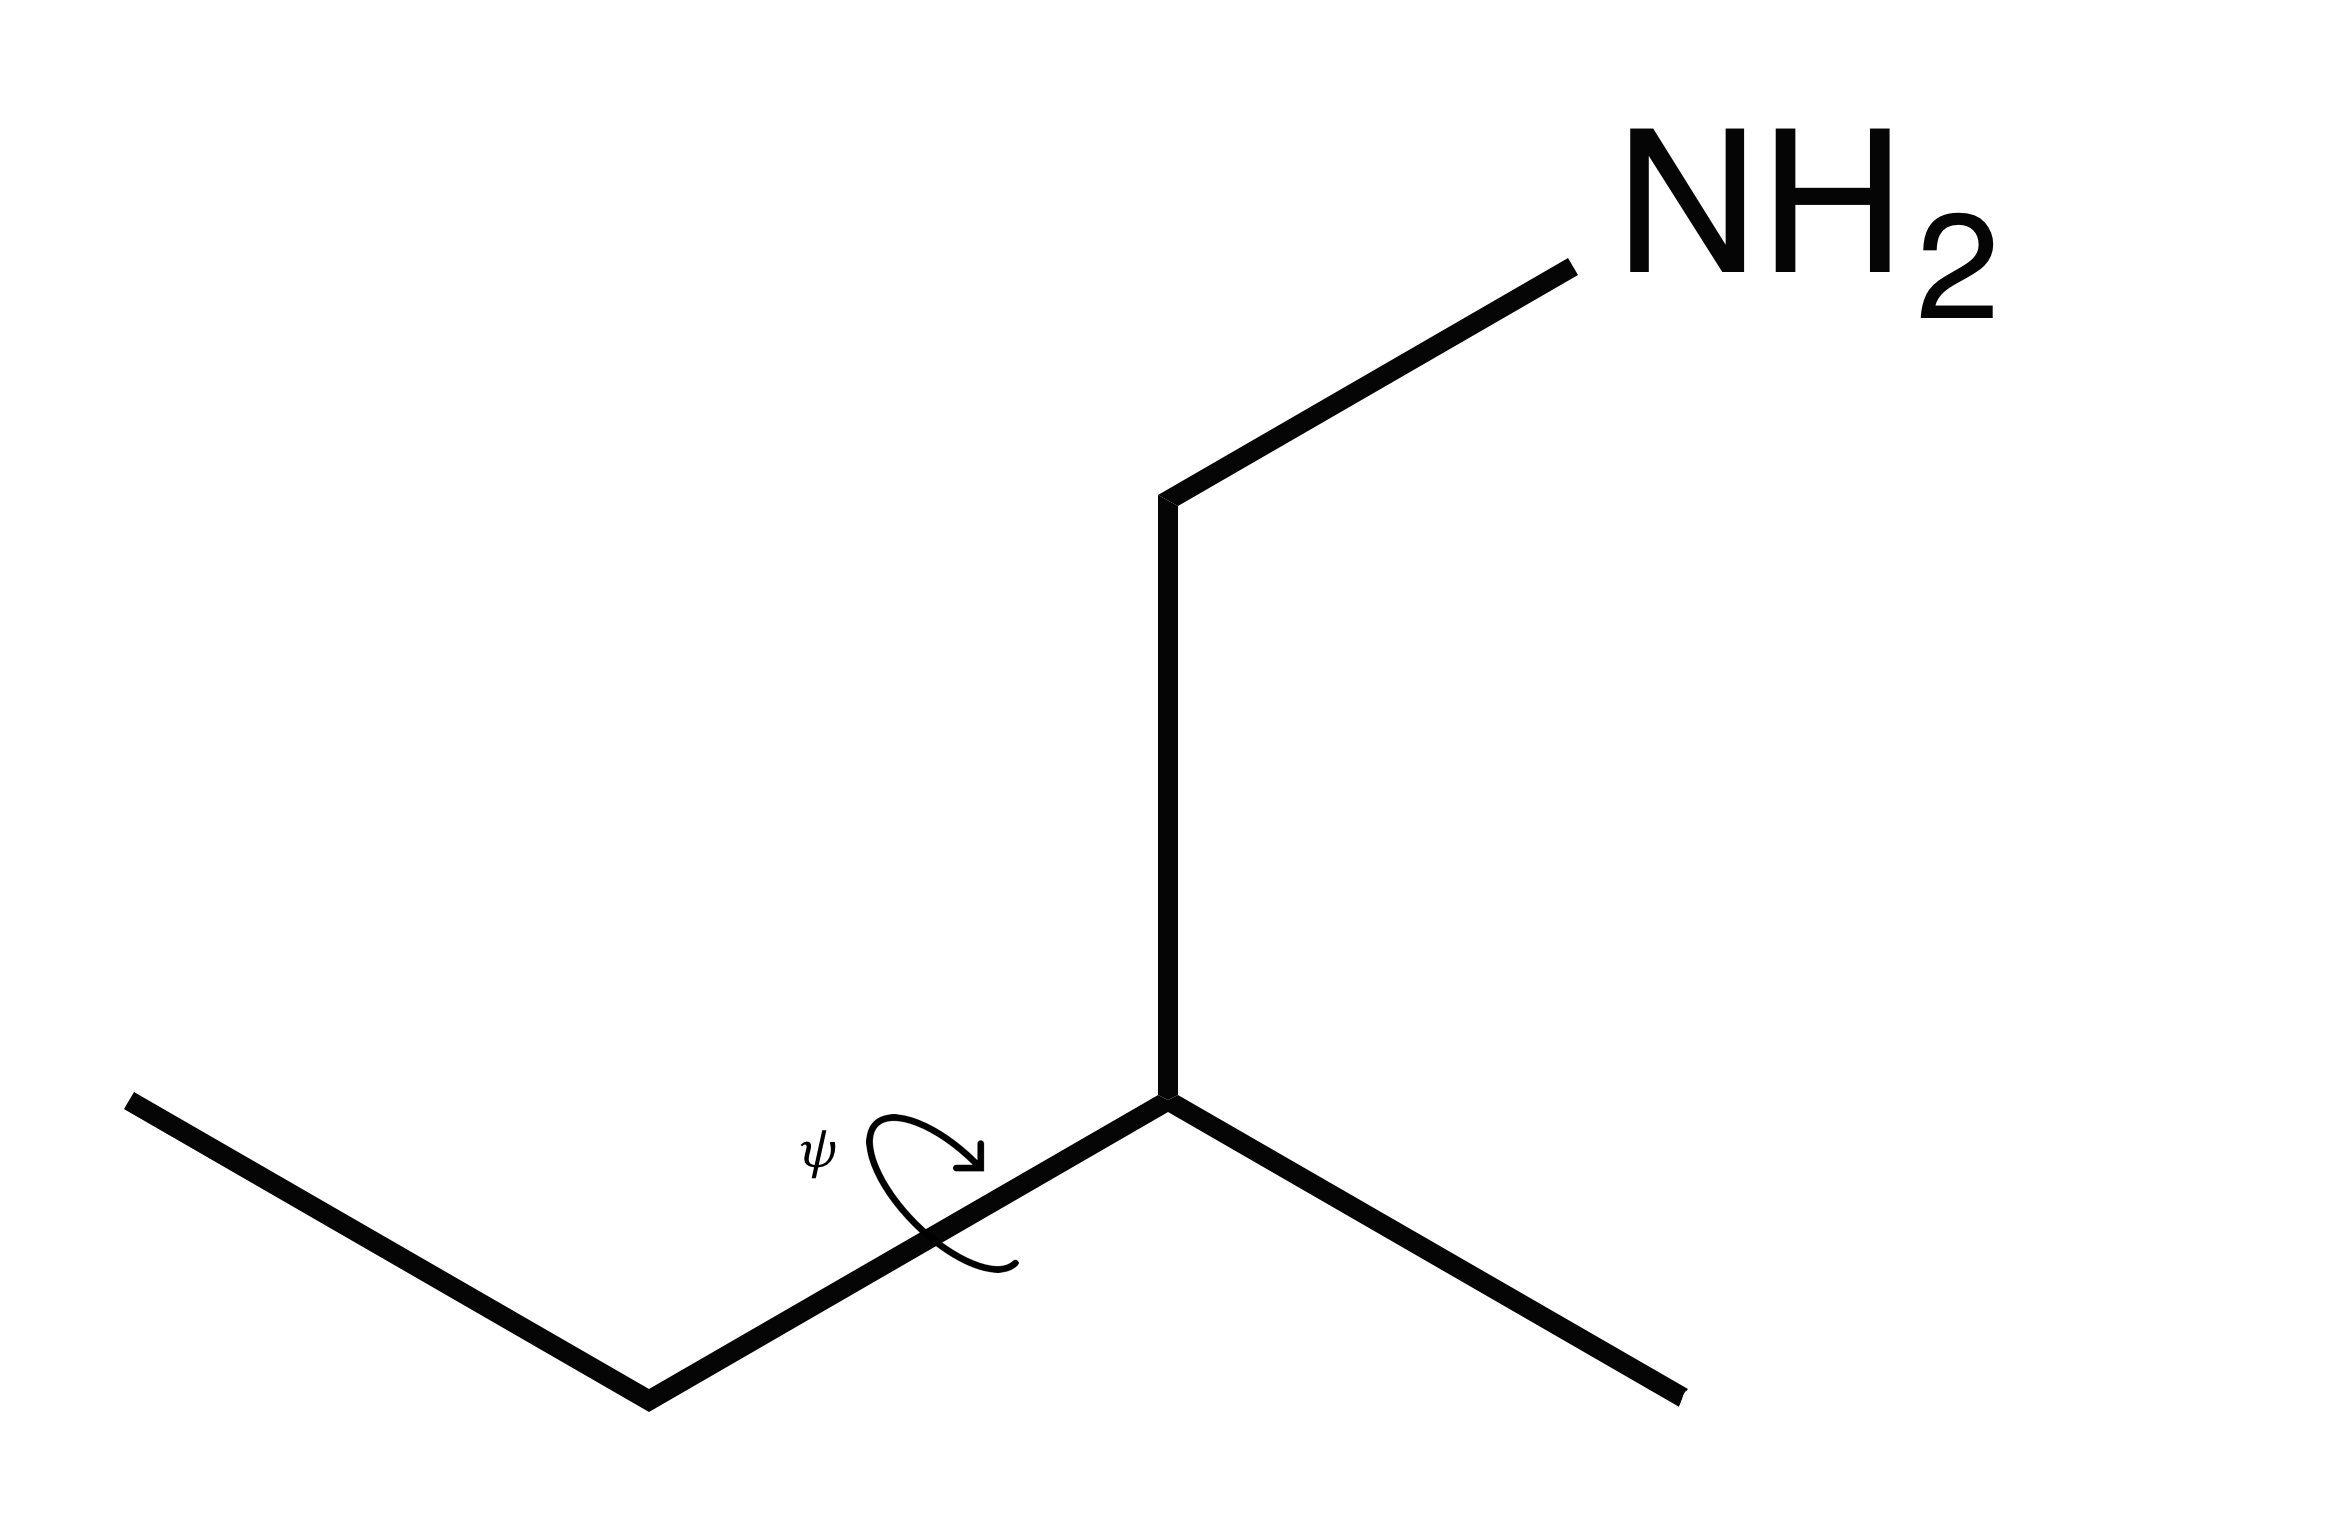
\includegraphics[scale=0.05]{Images/amino-1} & 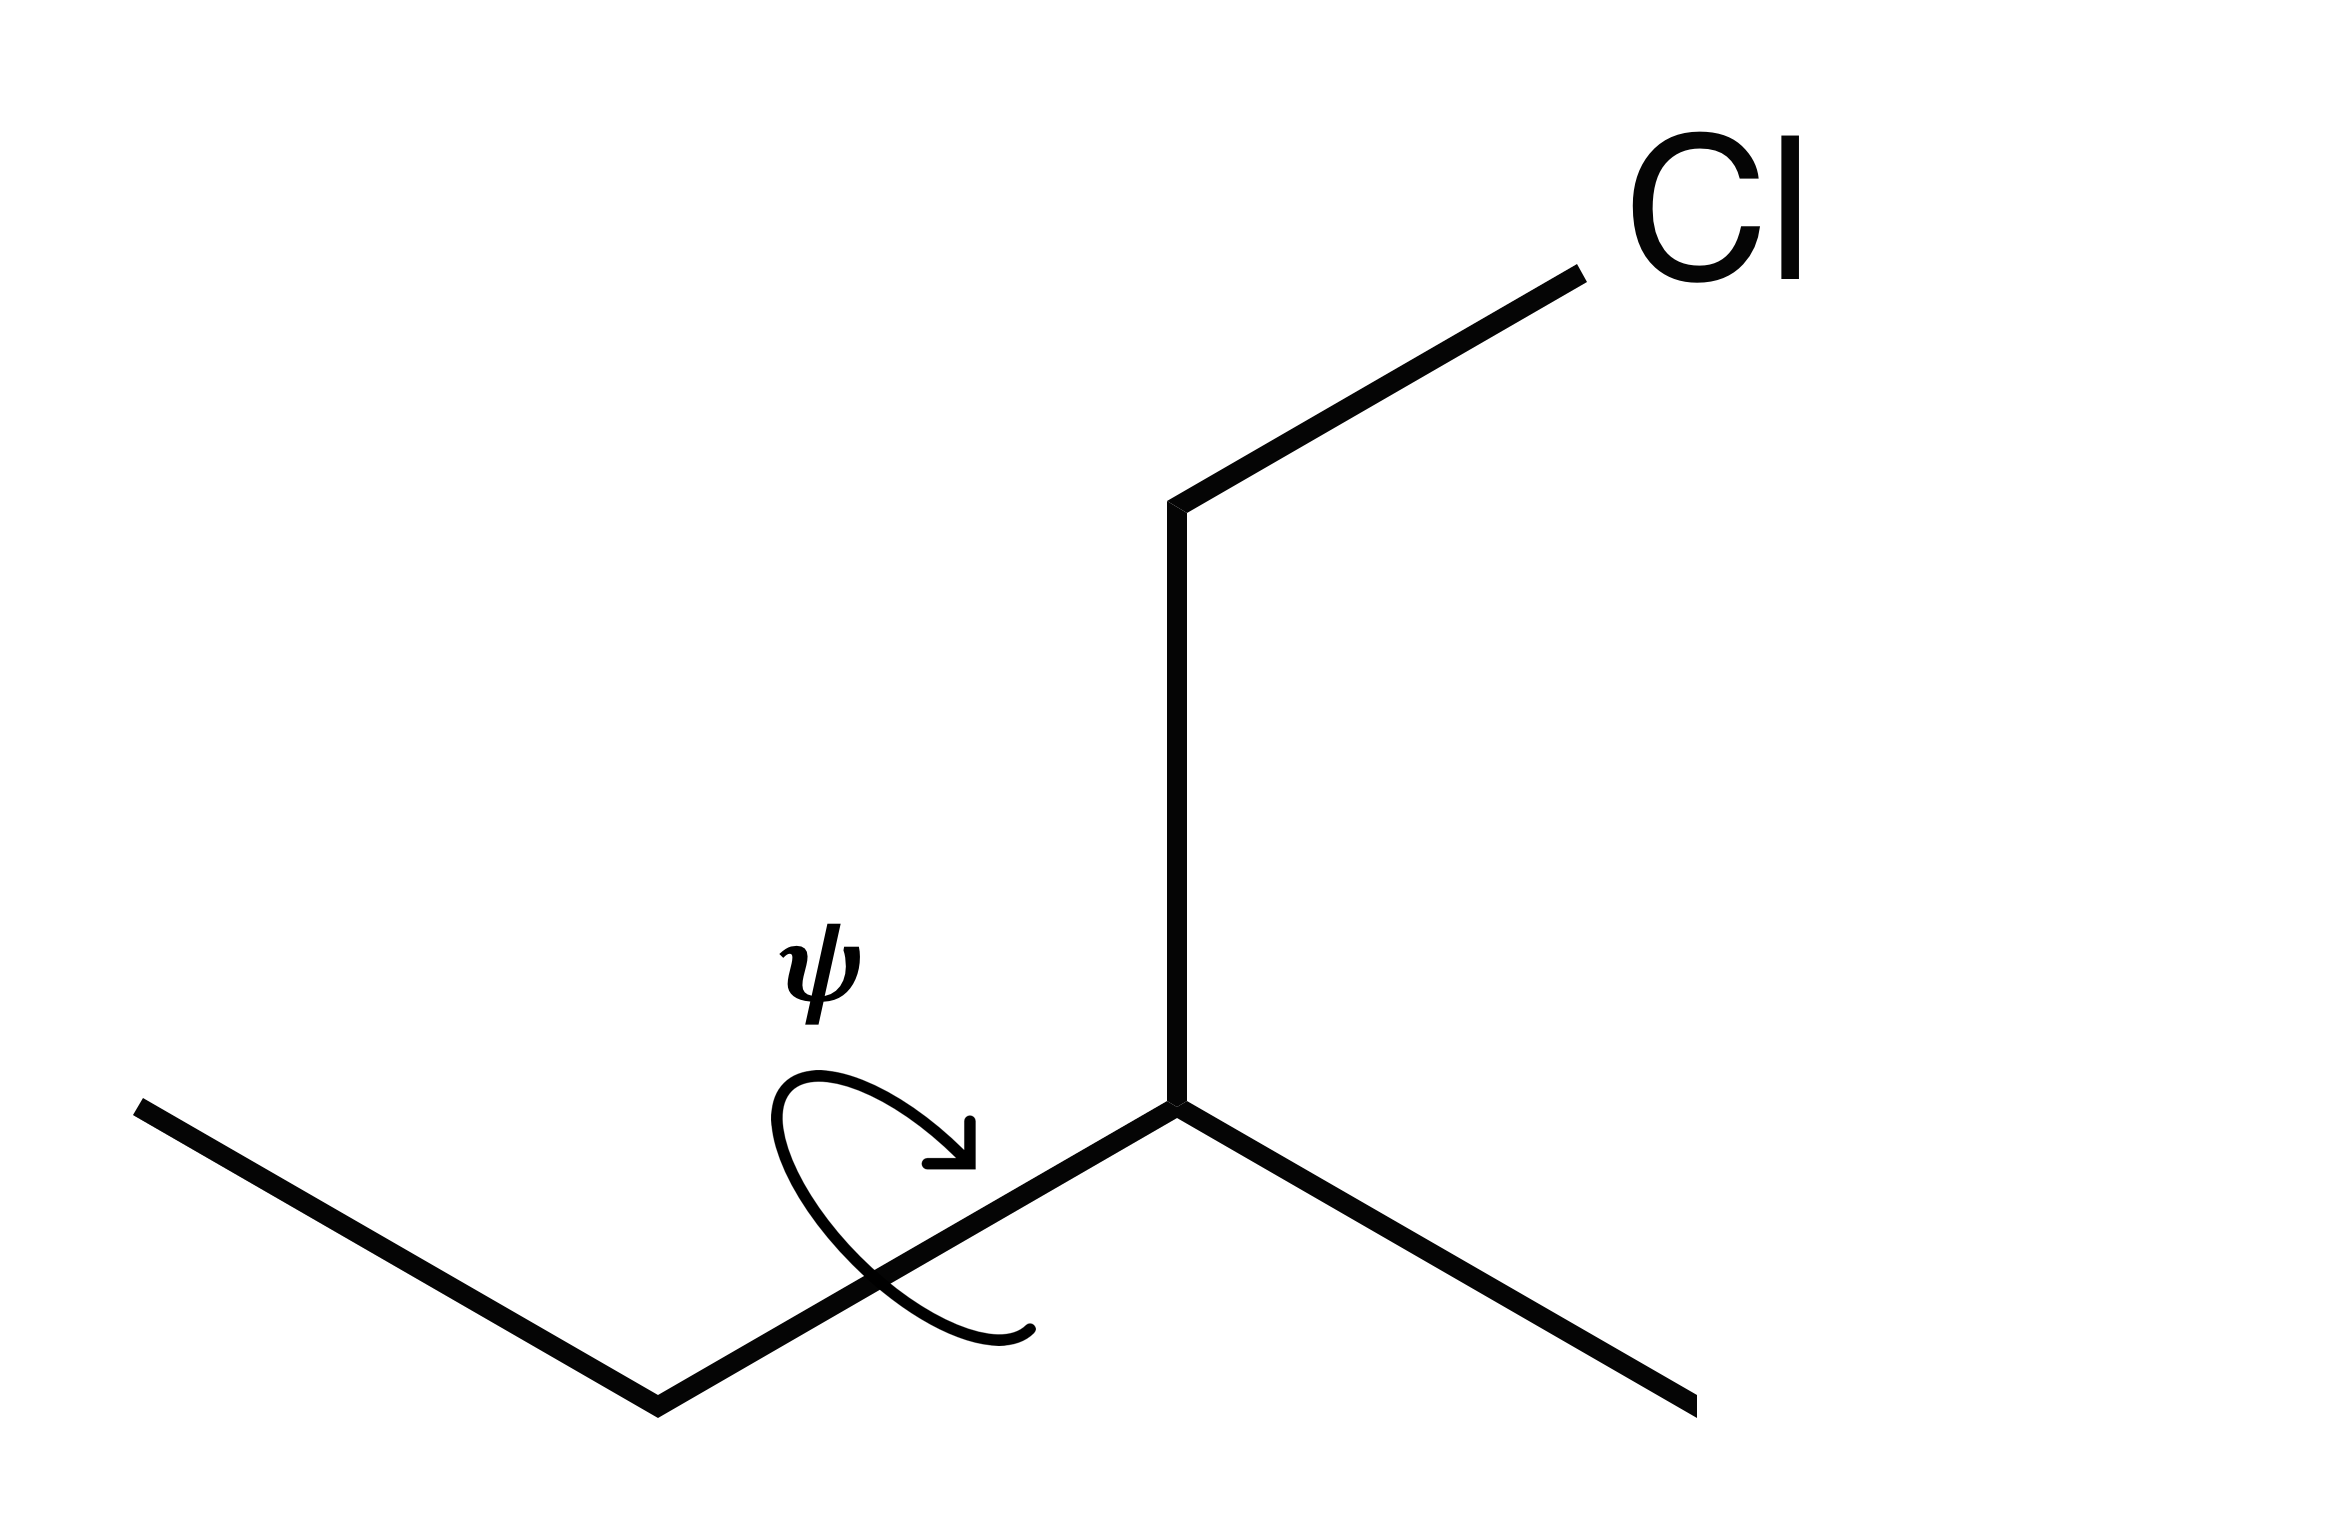
\includegraphics[scale=0.05]{Images/chloro-1} & 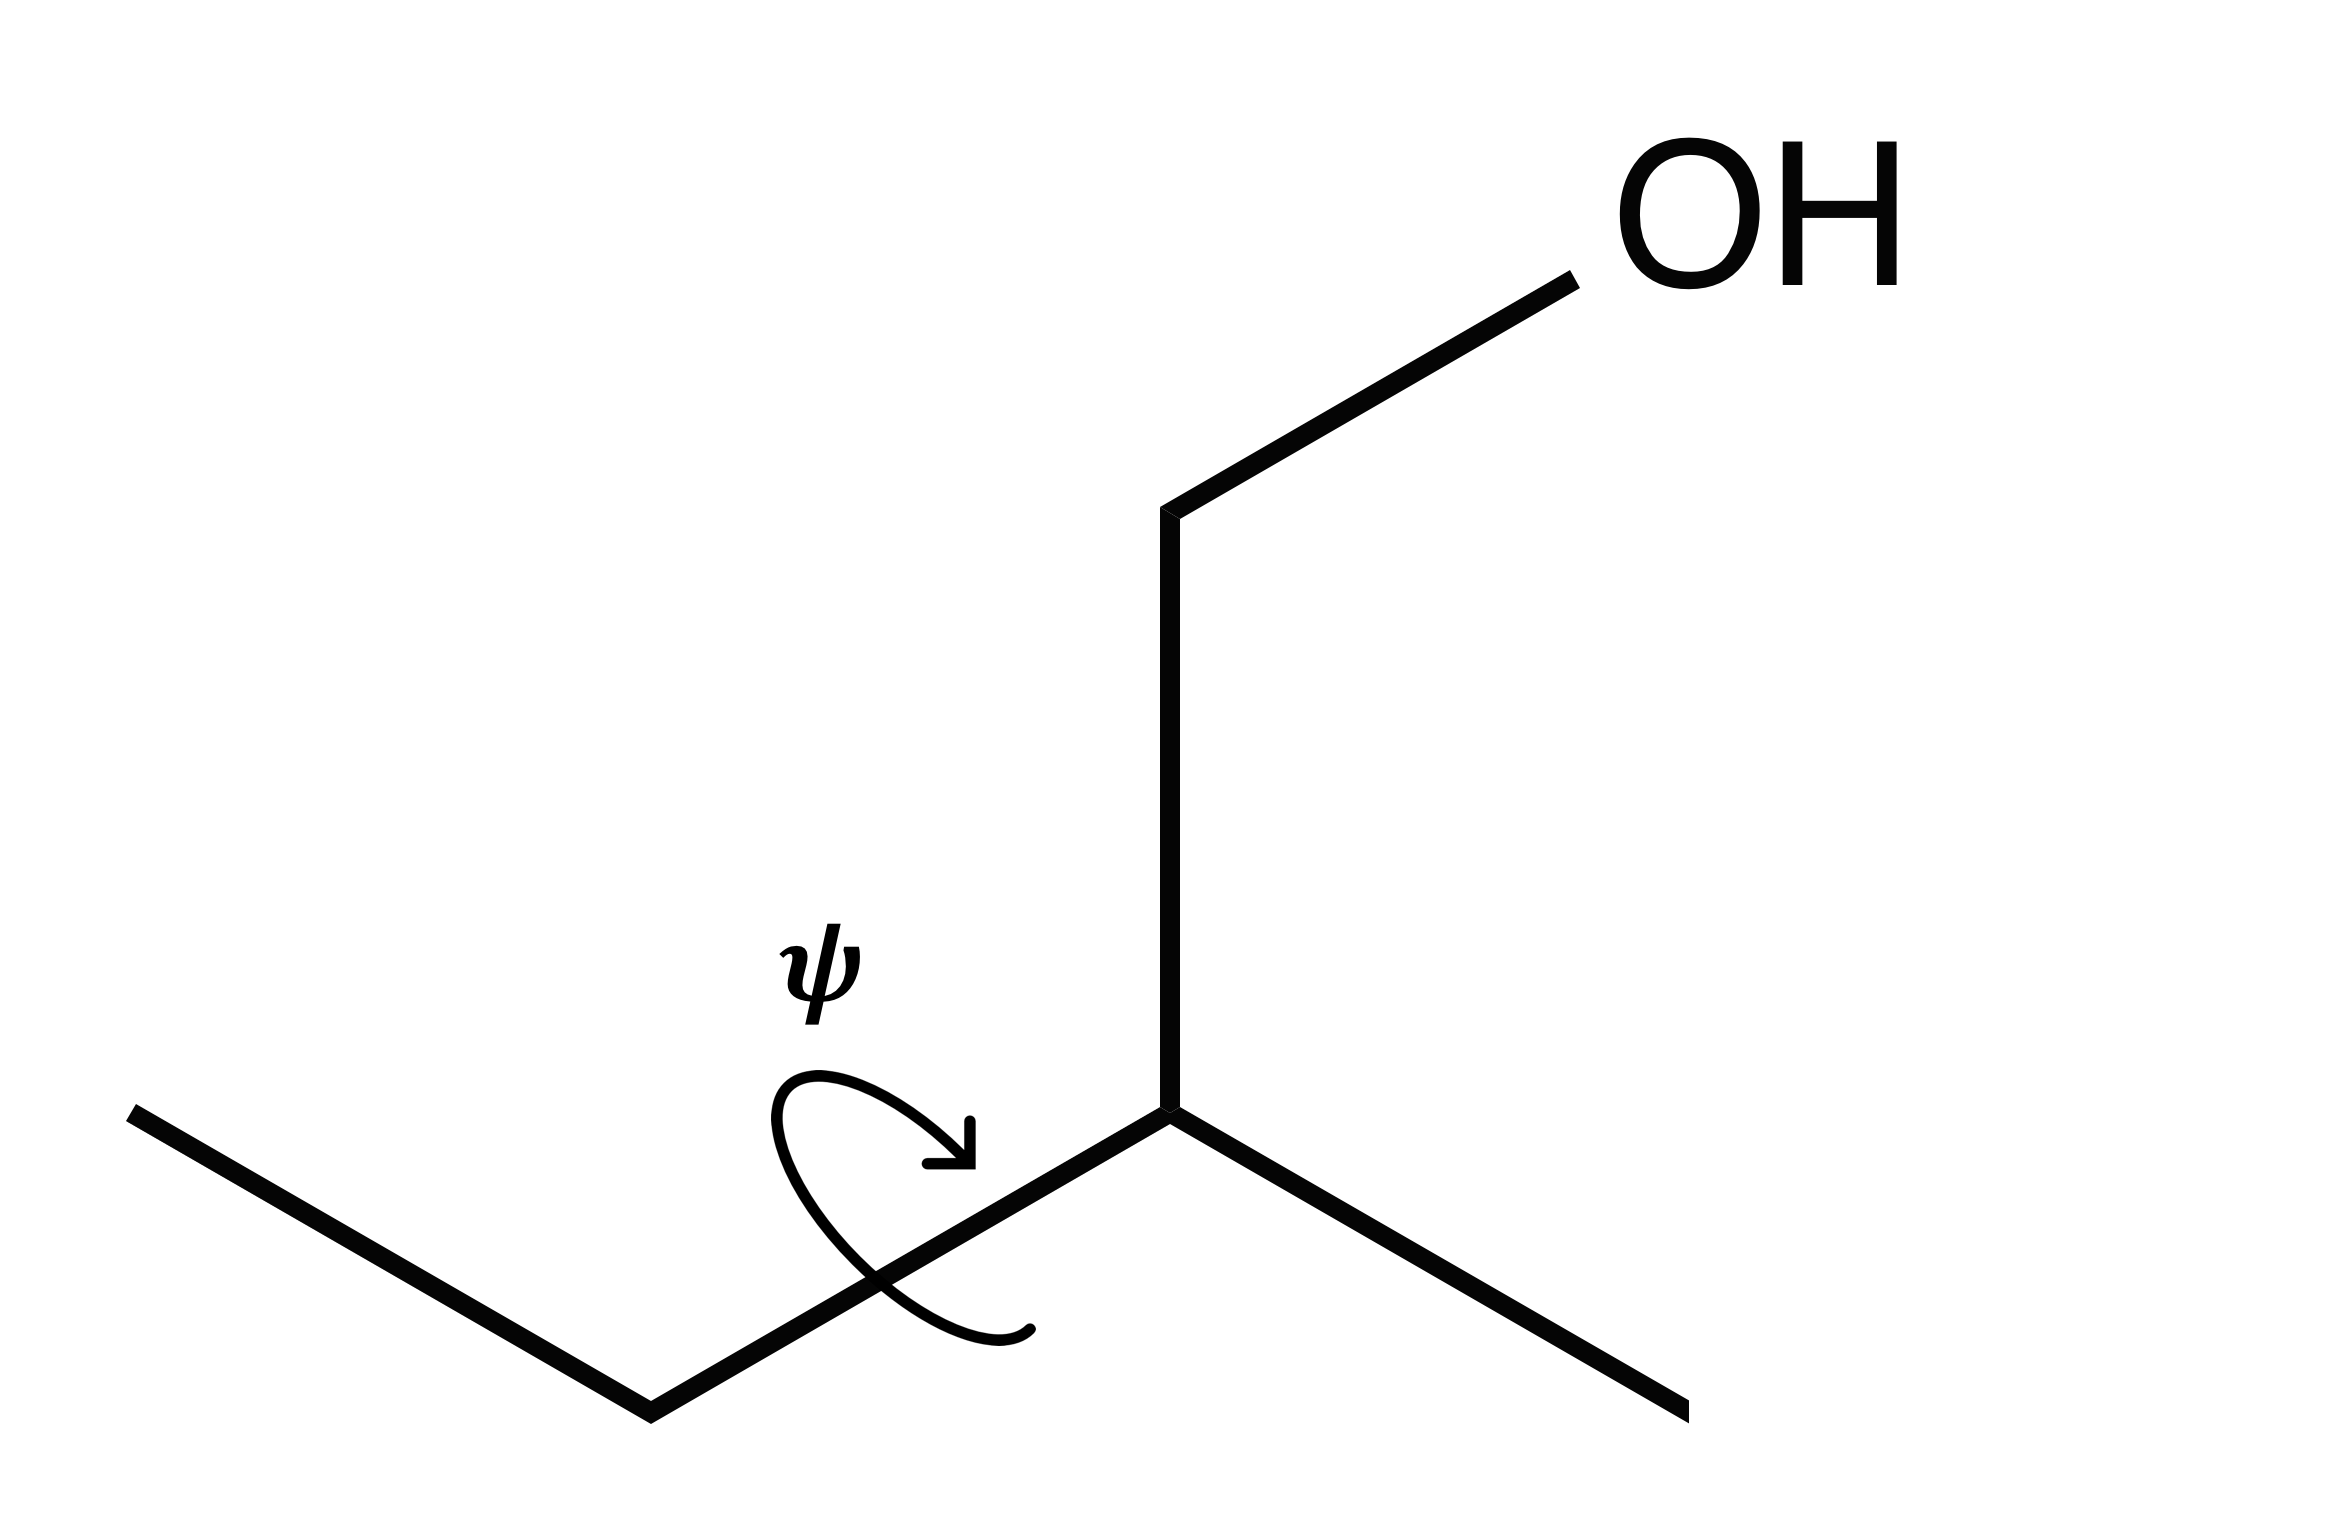
\includegraphics[scale=0.05]{Images/hydro-1} & 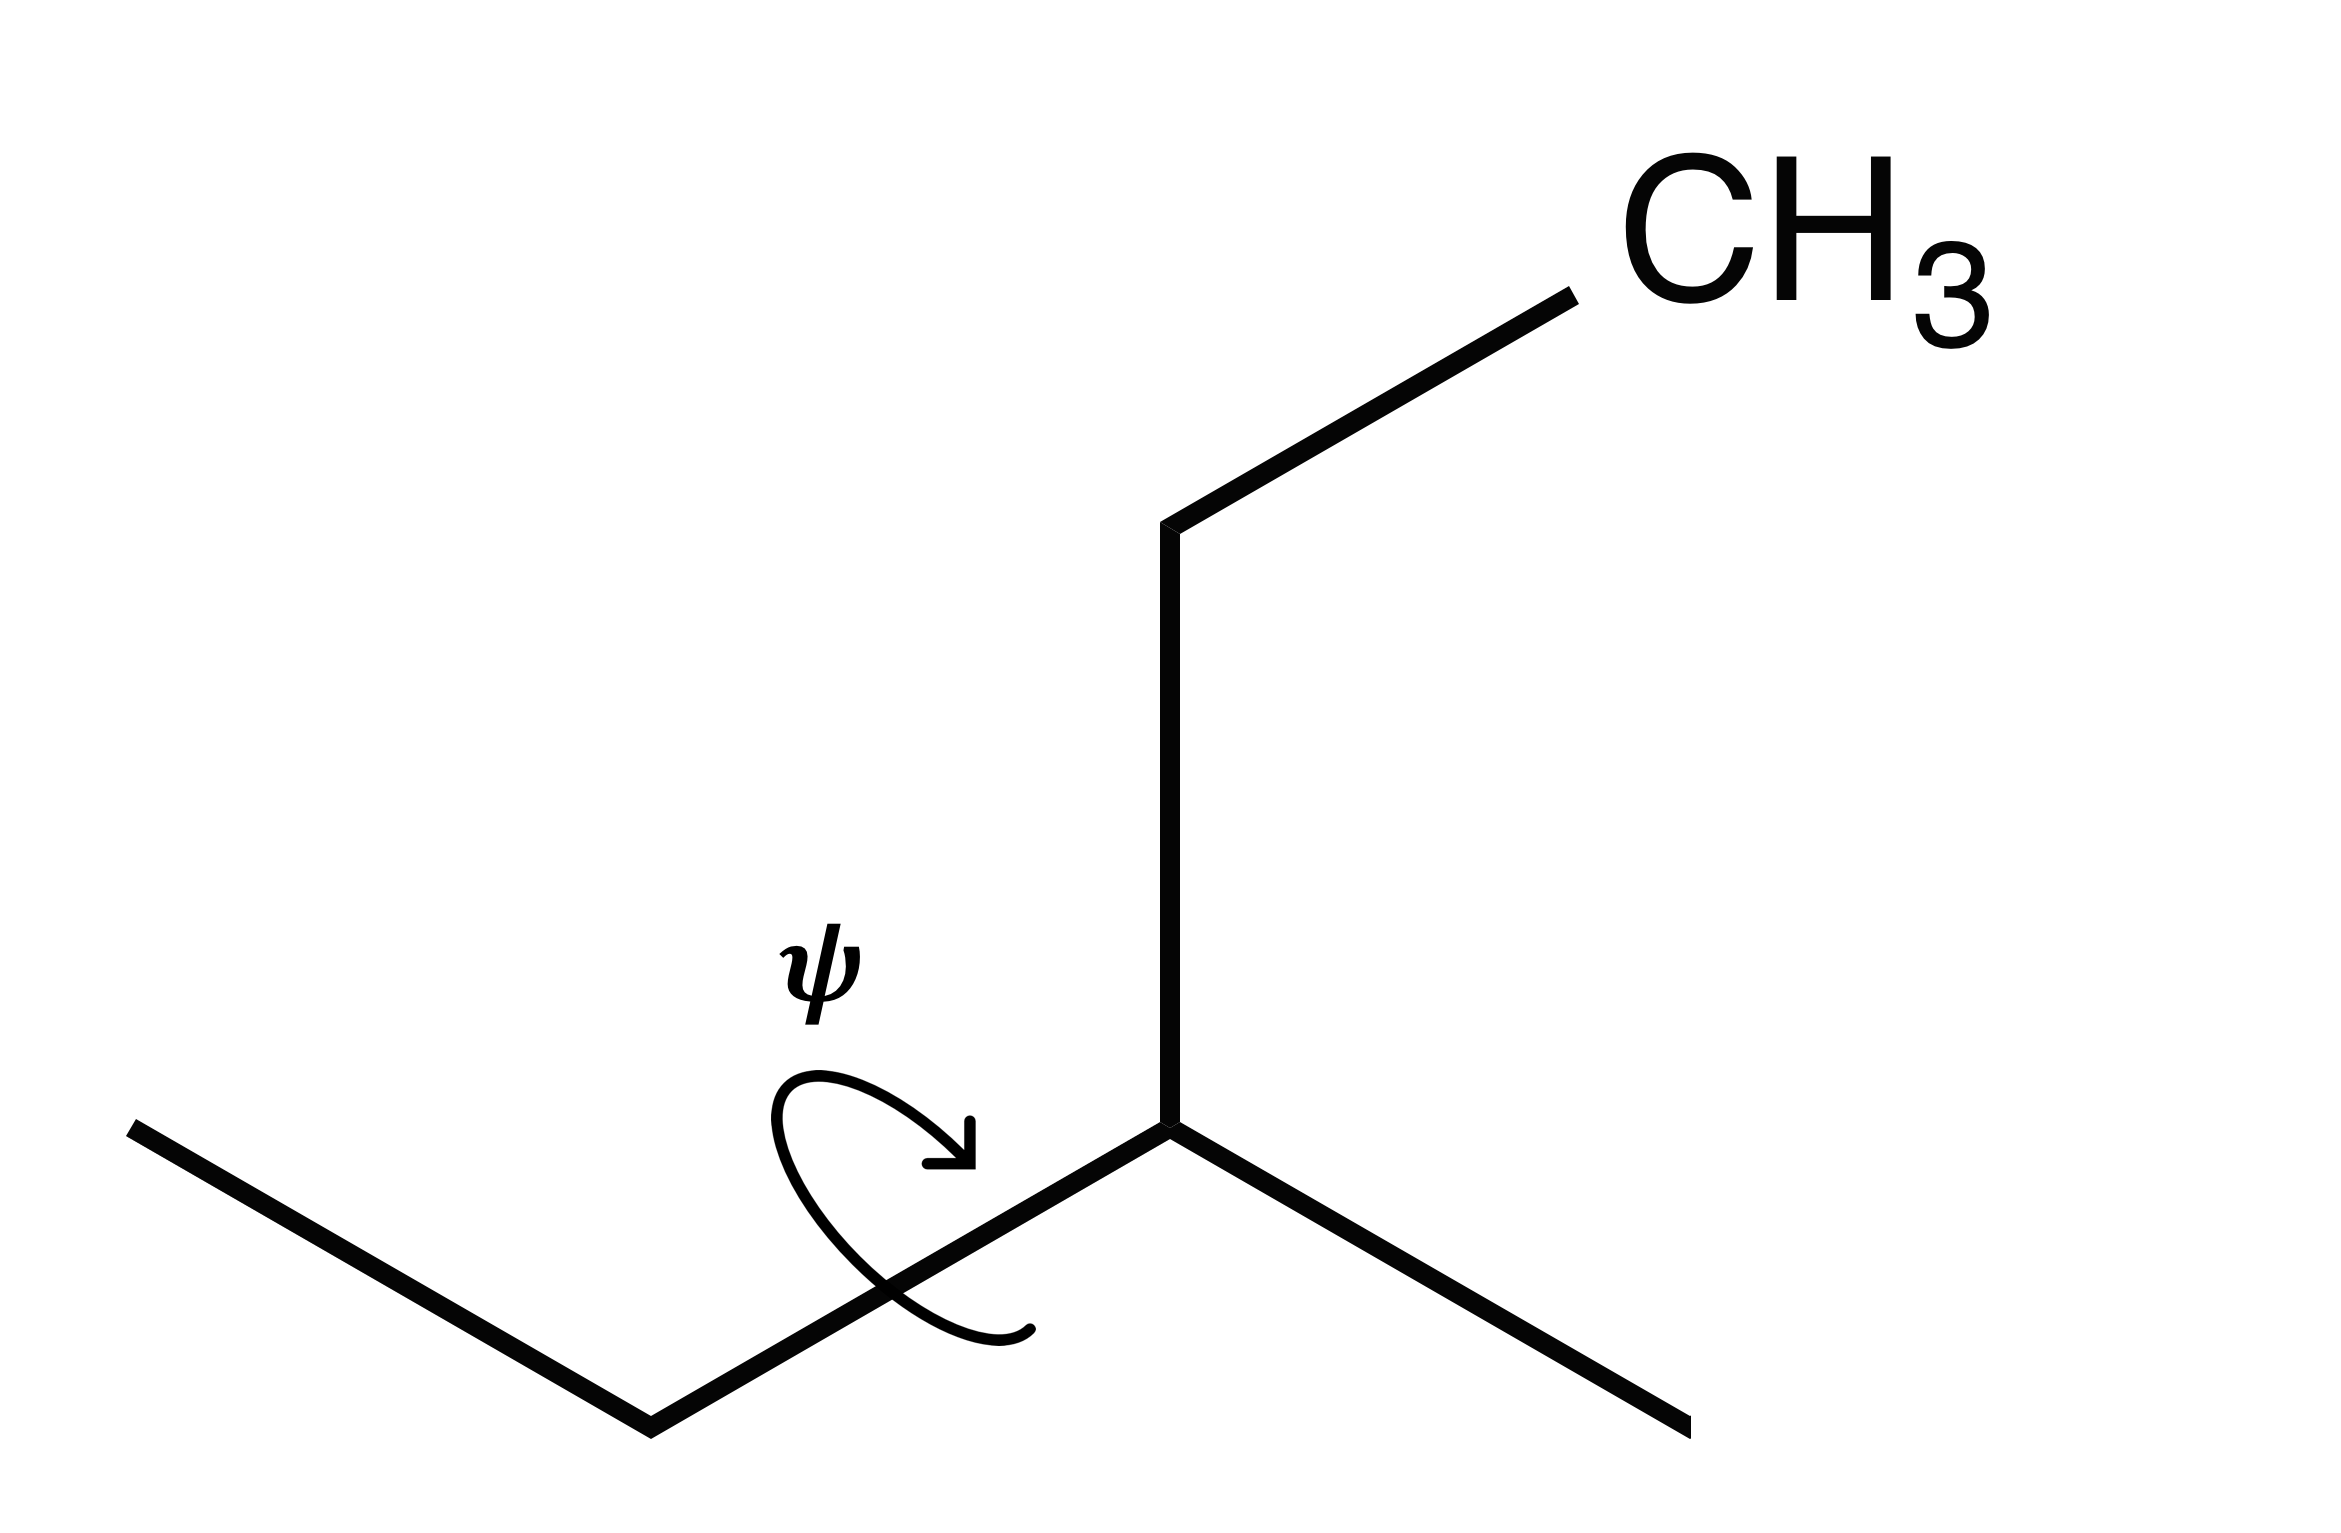
\includegraphics[scale=0.05]{Images/meth-1} & 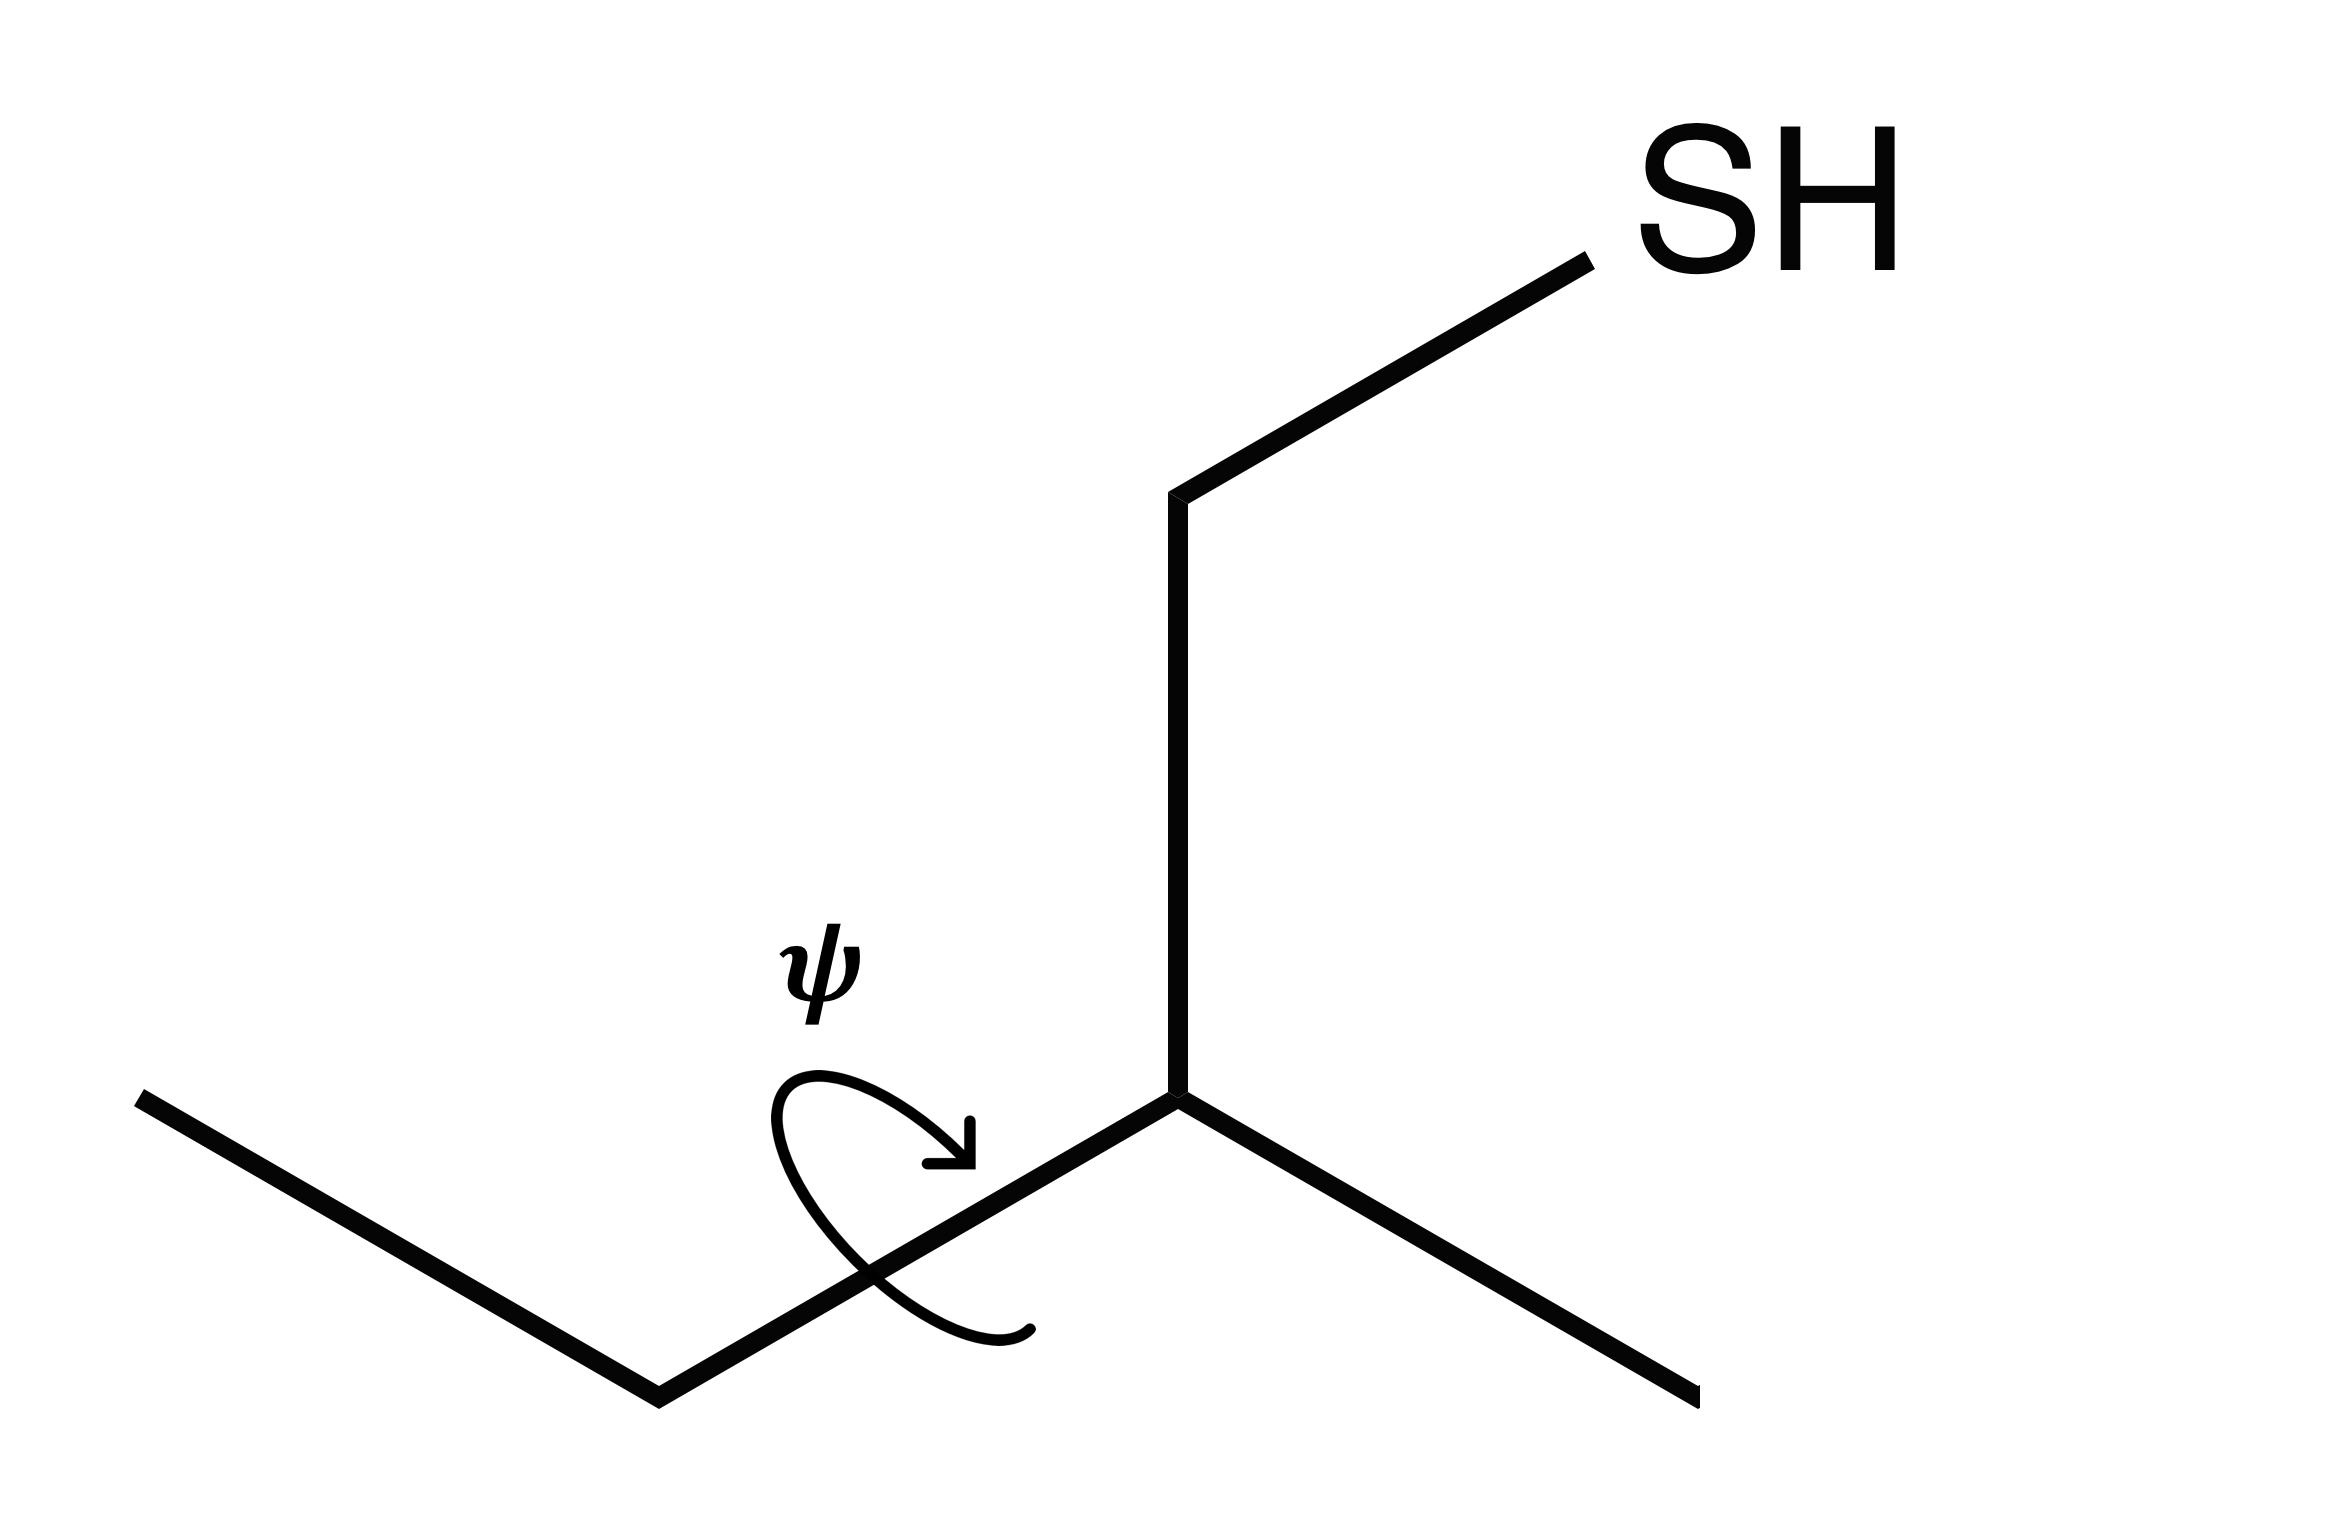
\includegraphics[scale=0.05]{Images/thio-1} \\
 & 28471 & 28472 & 28473 & 756 & 28474 \\ \hline
\multirow{2}{*}{0} & 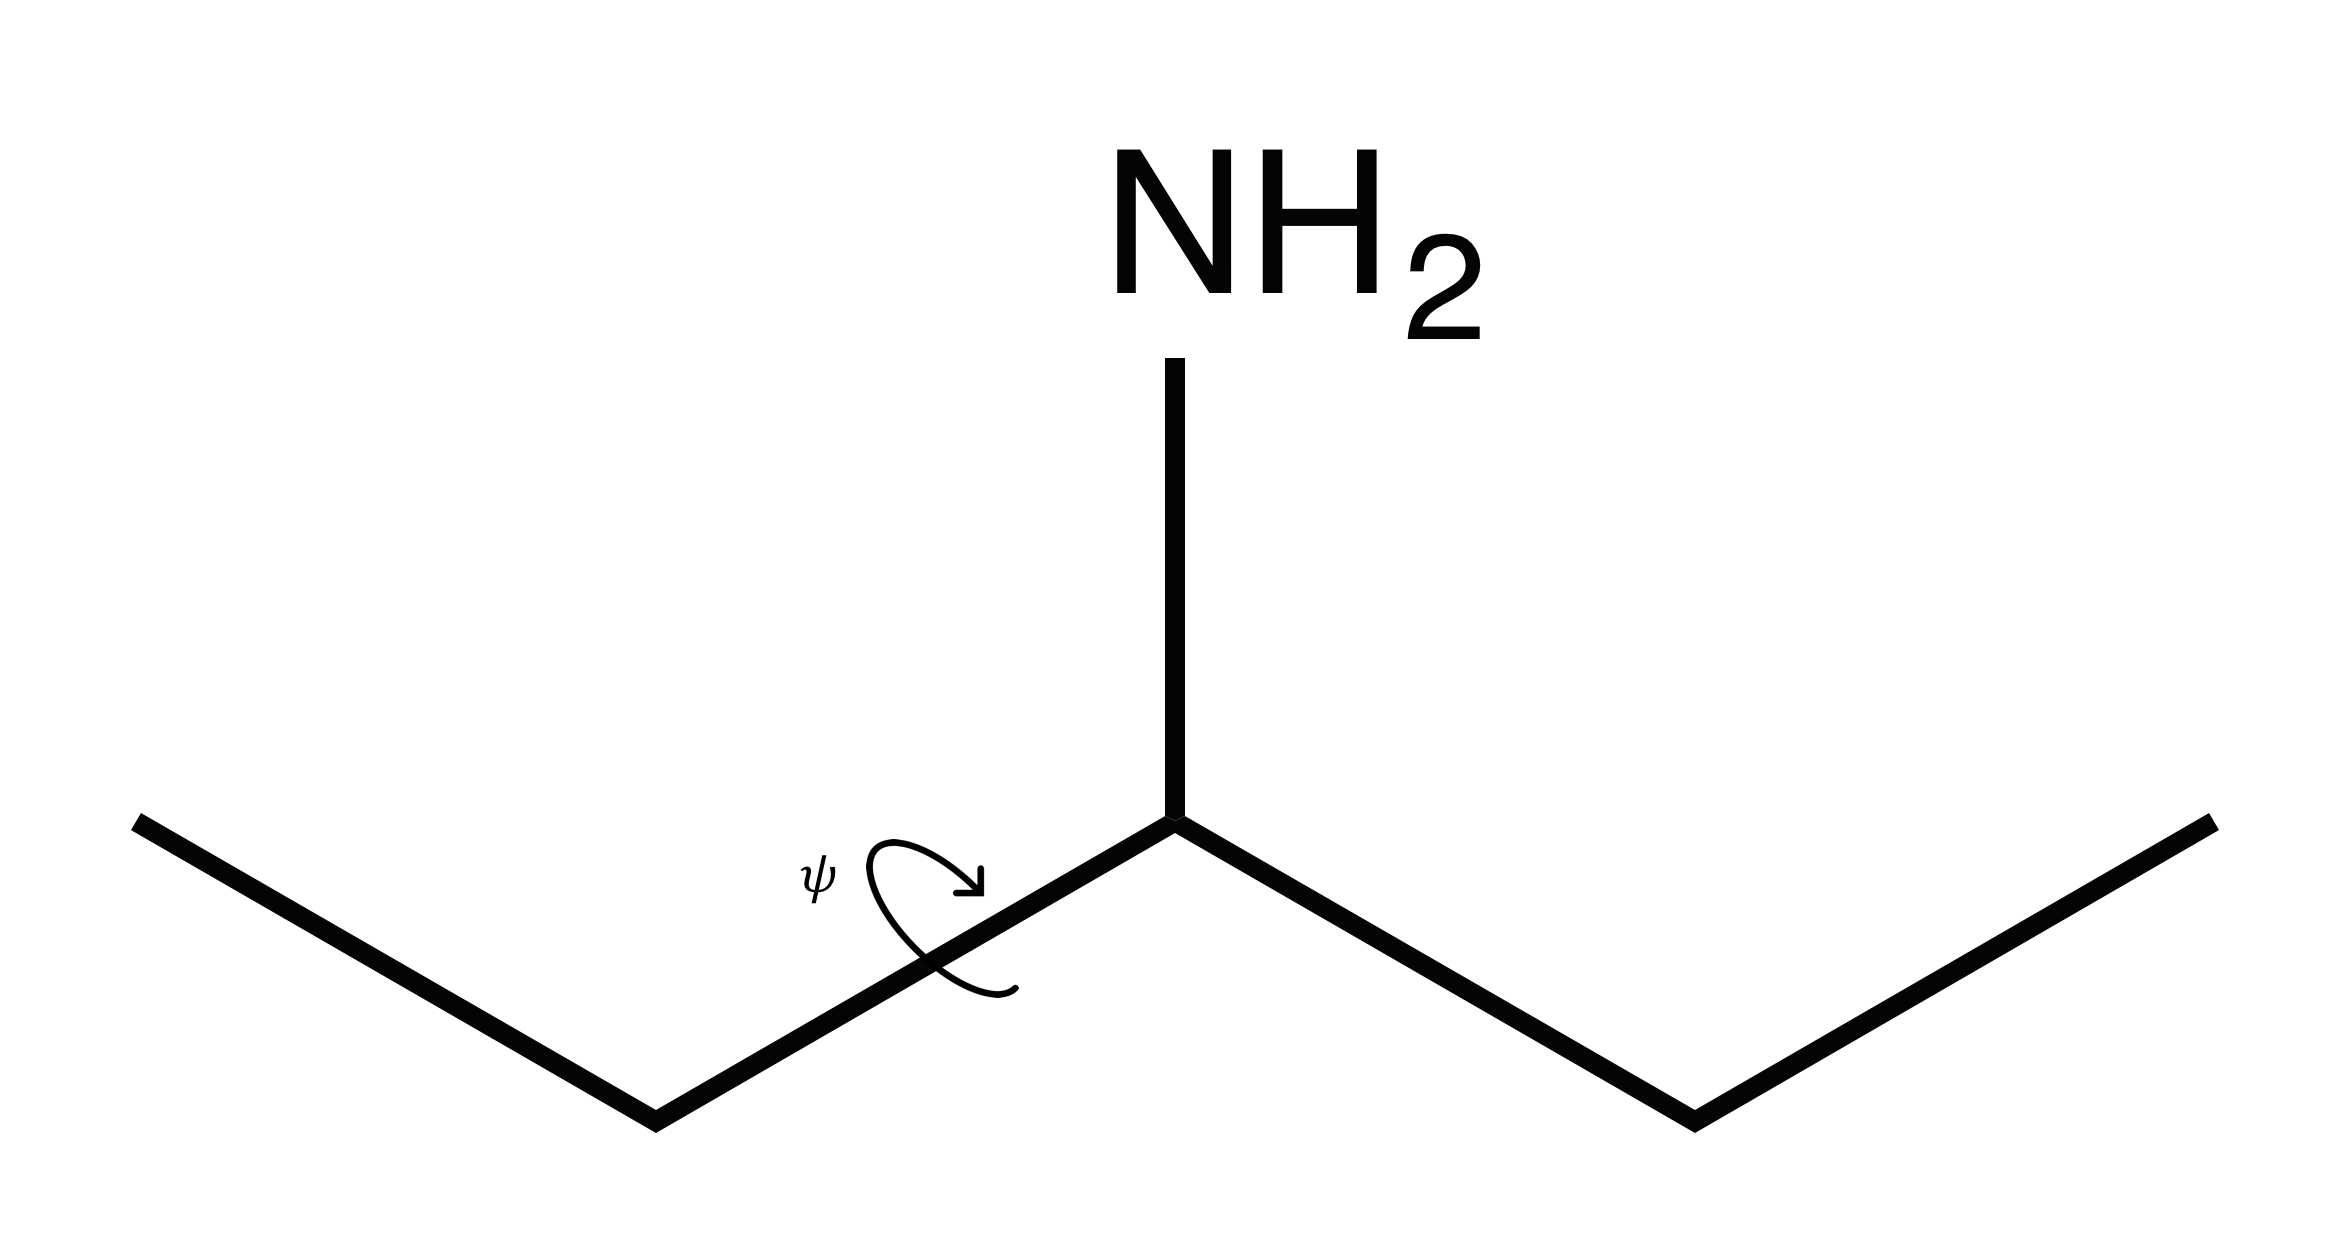
\includegraphics[scale=0.05]{Images/amino0} & 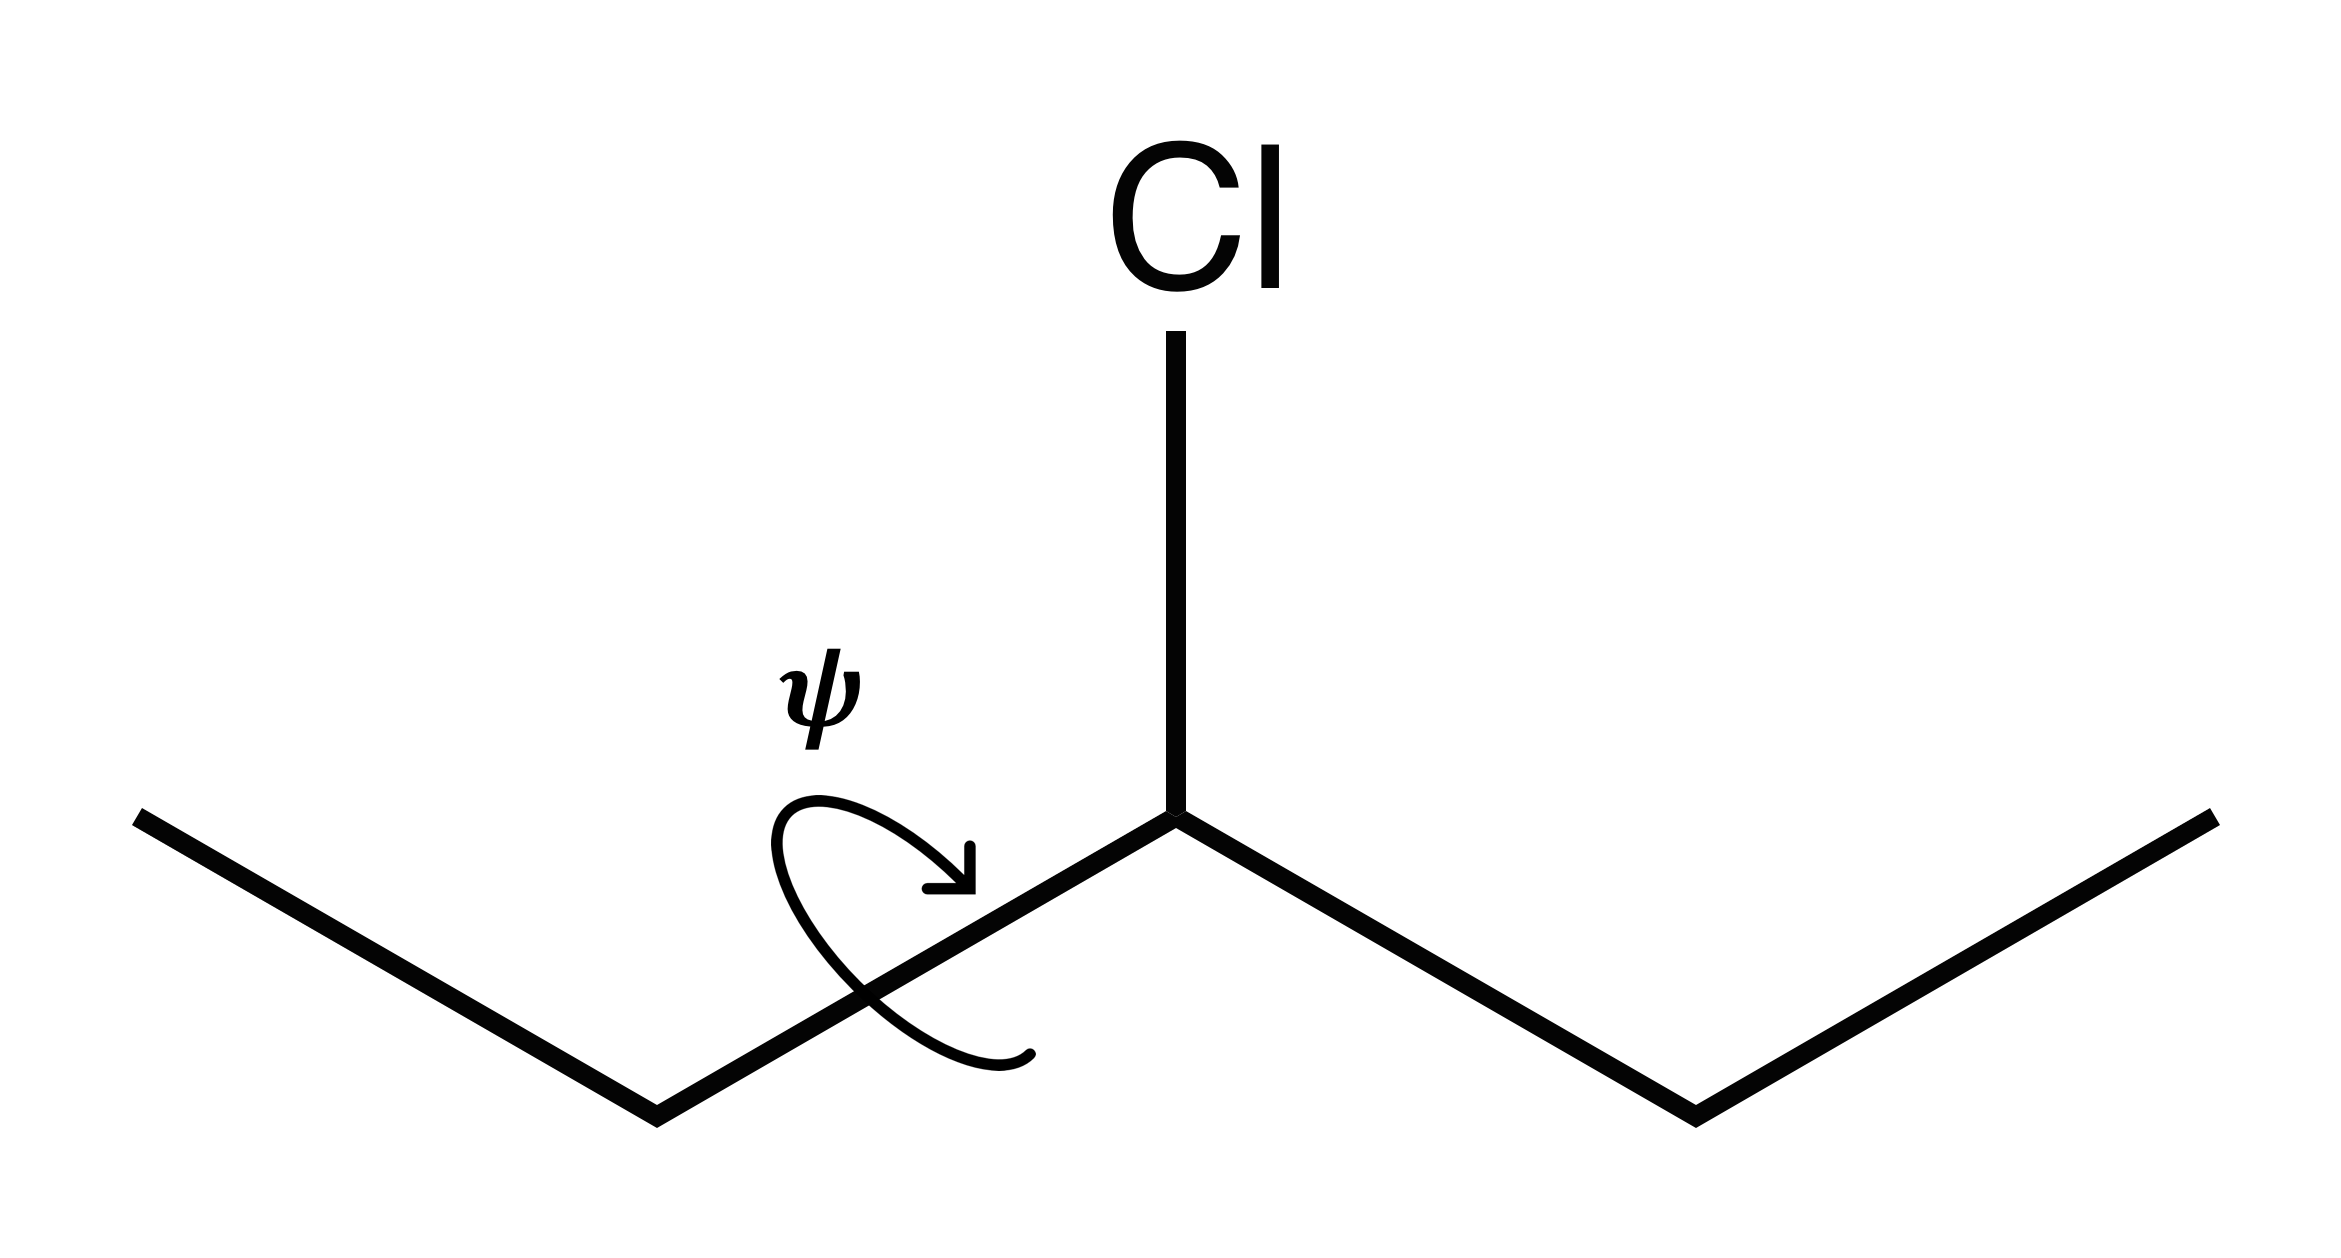
\includegraphics[scale=0.05]{Images/chloro0} & 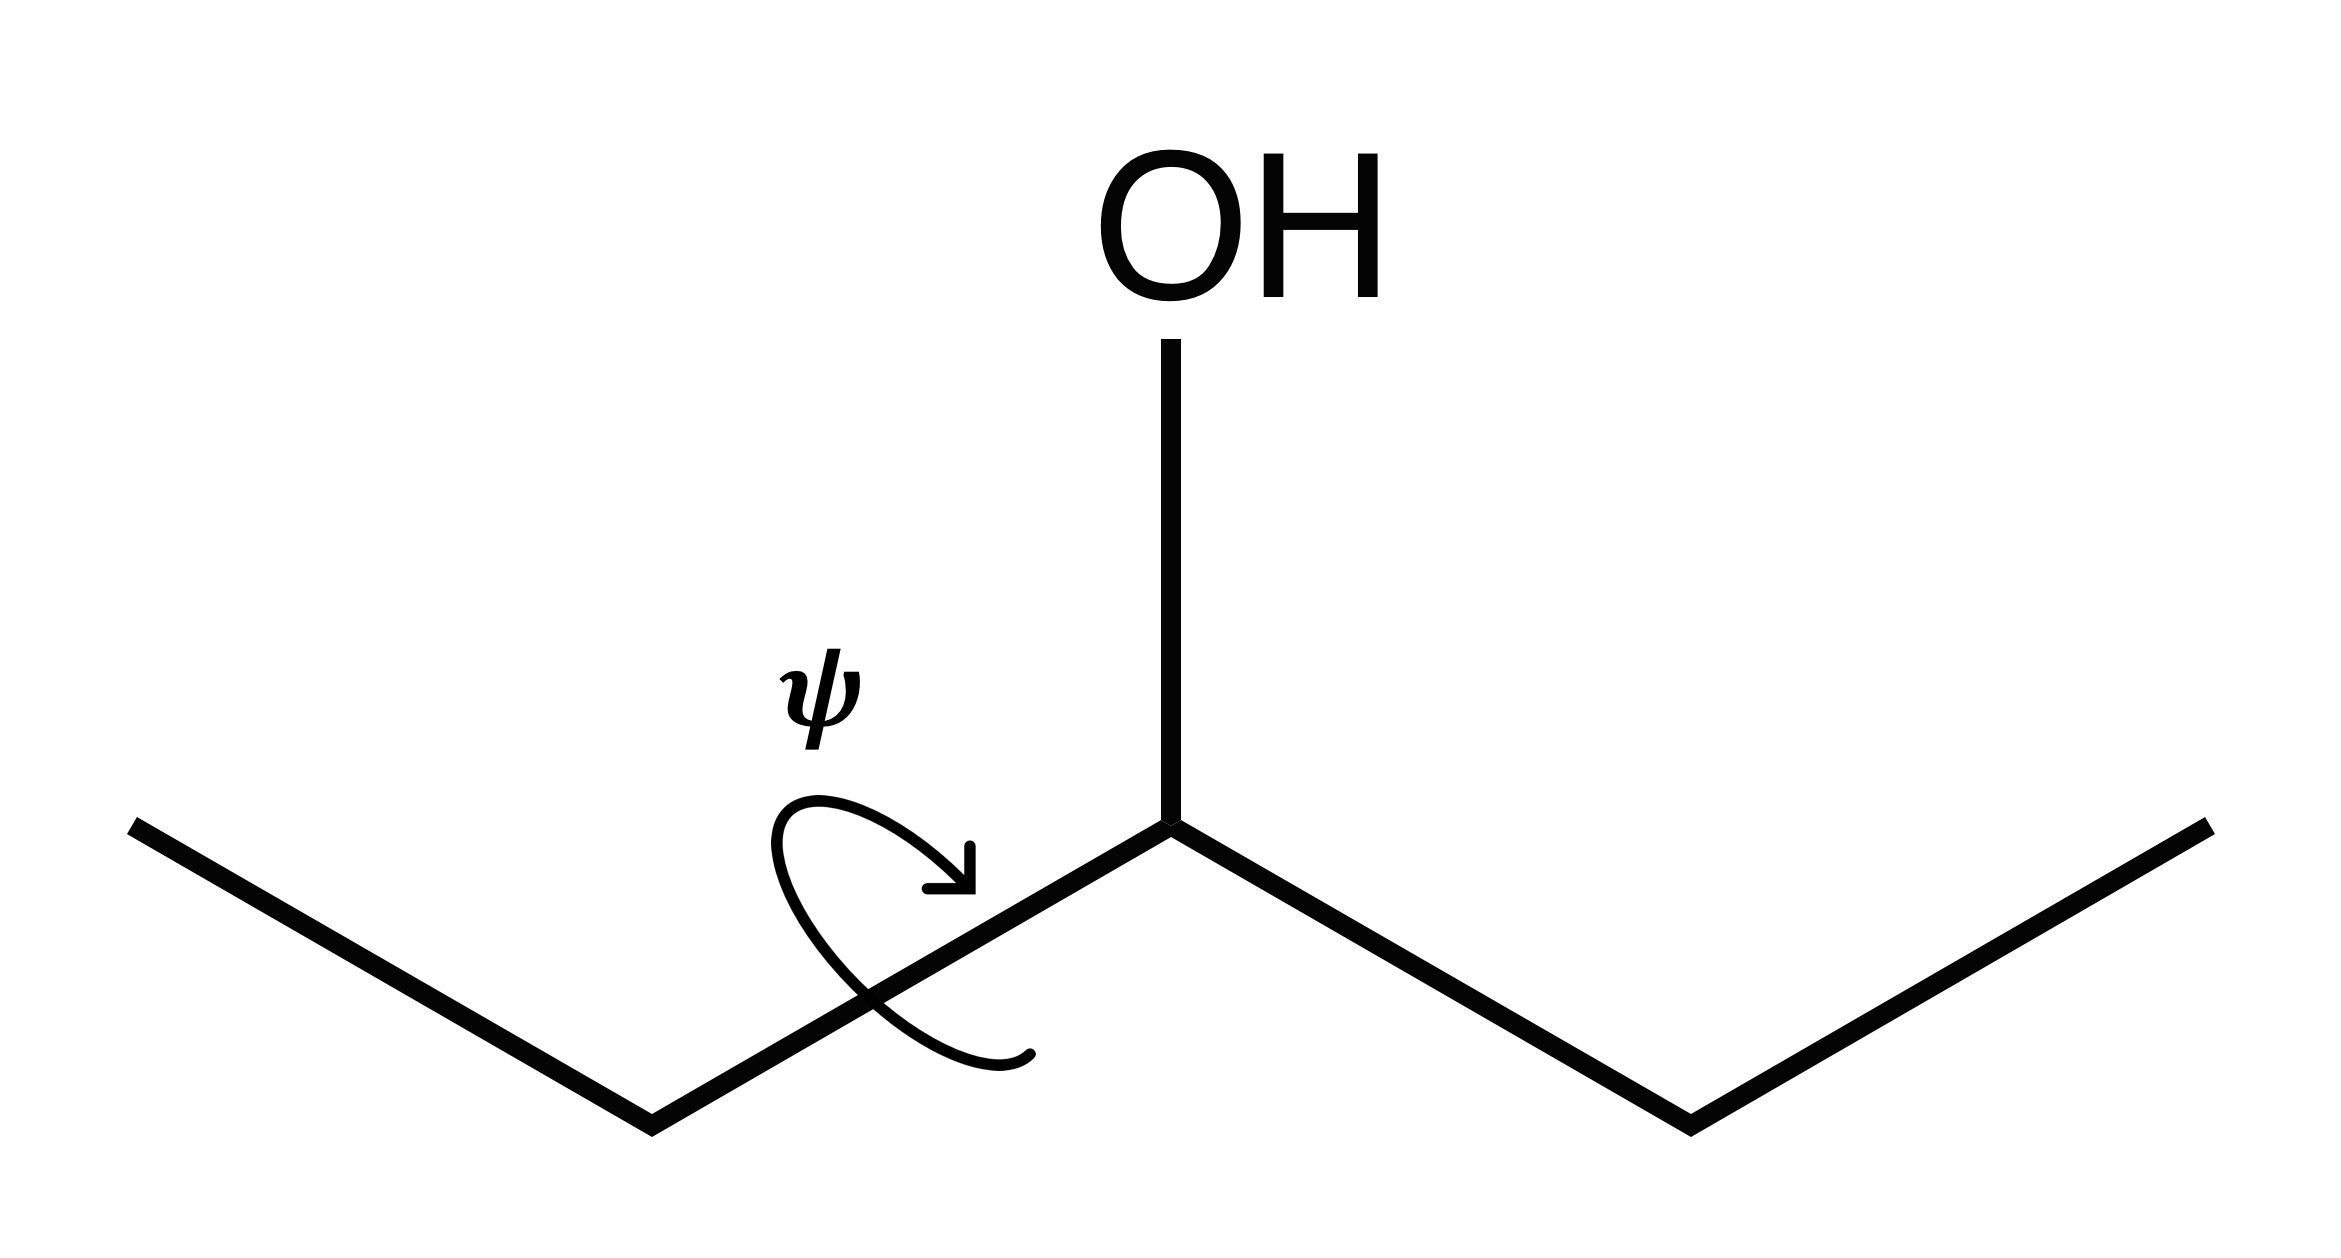
\includegraphics[scale=0.05]{Images/hydro0} & 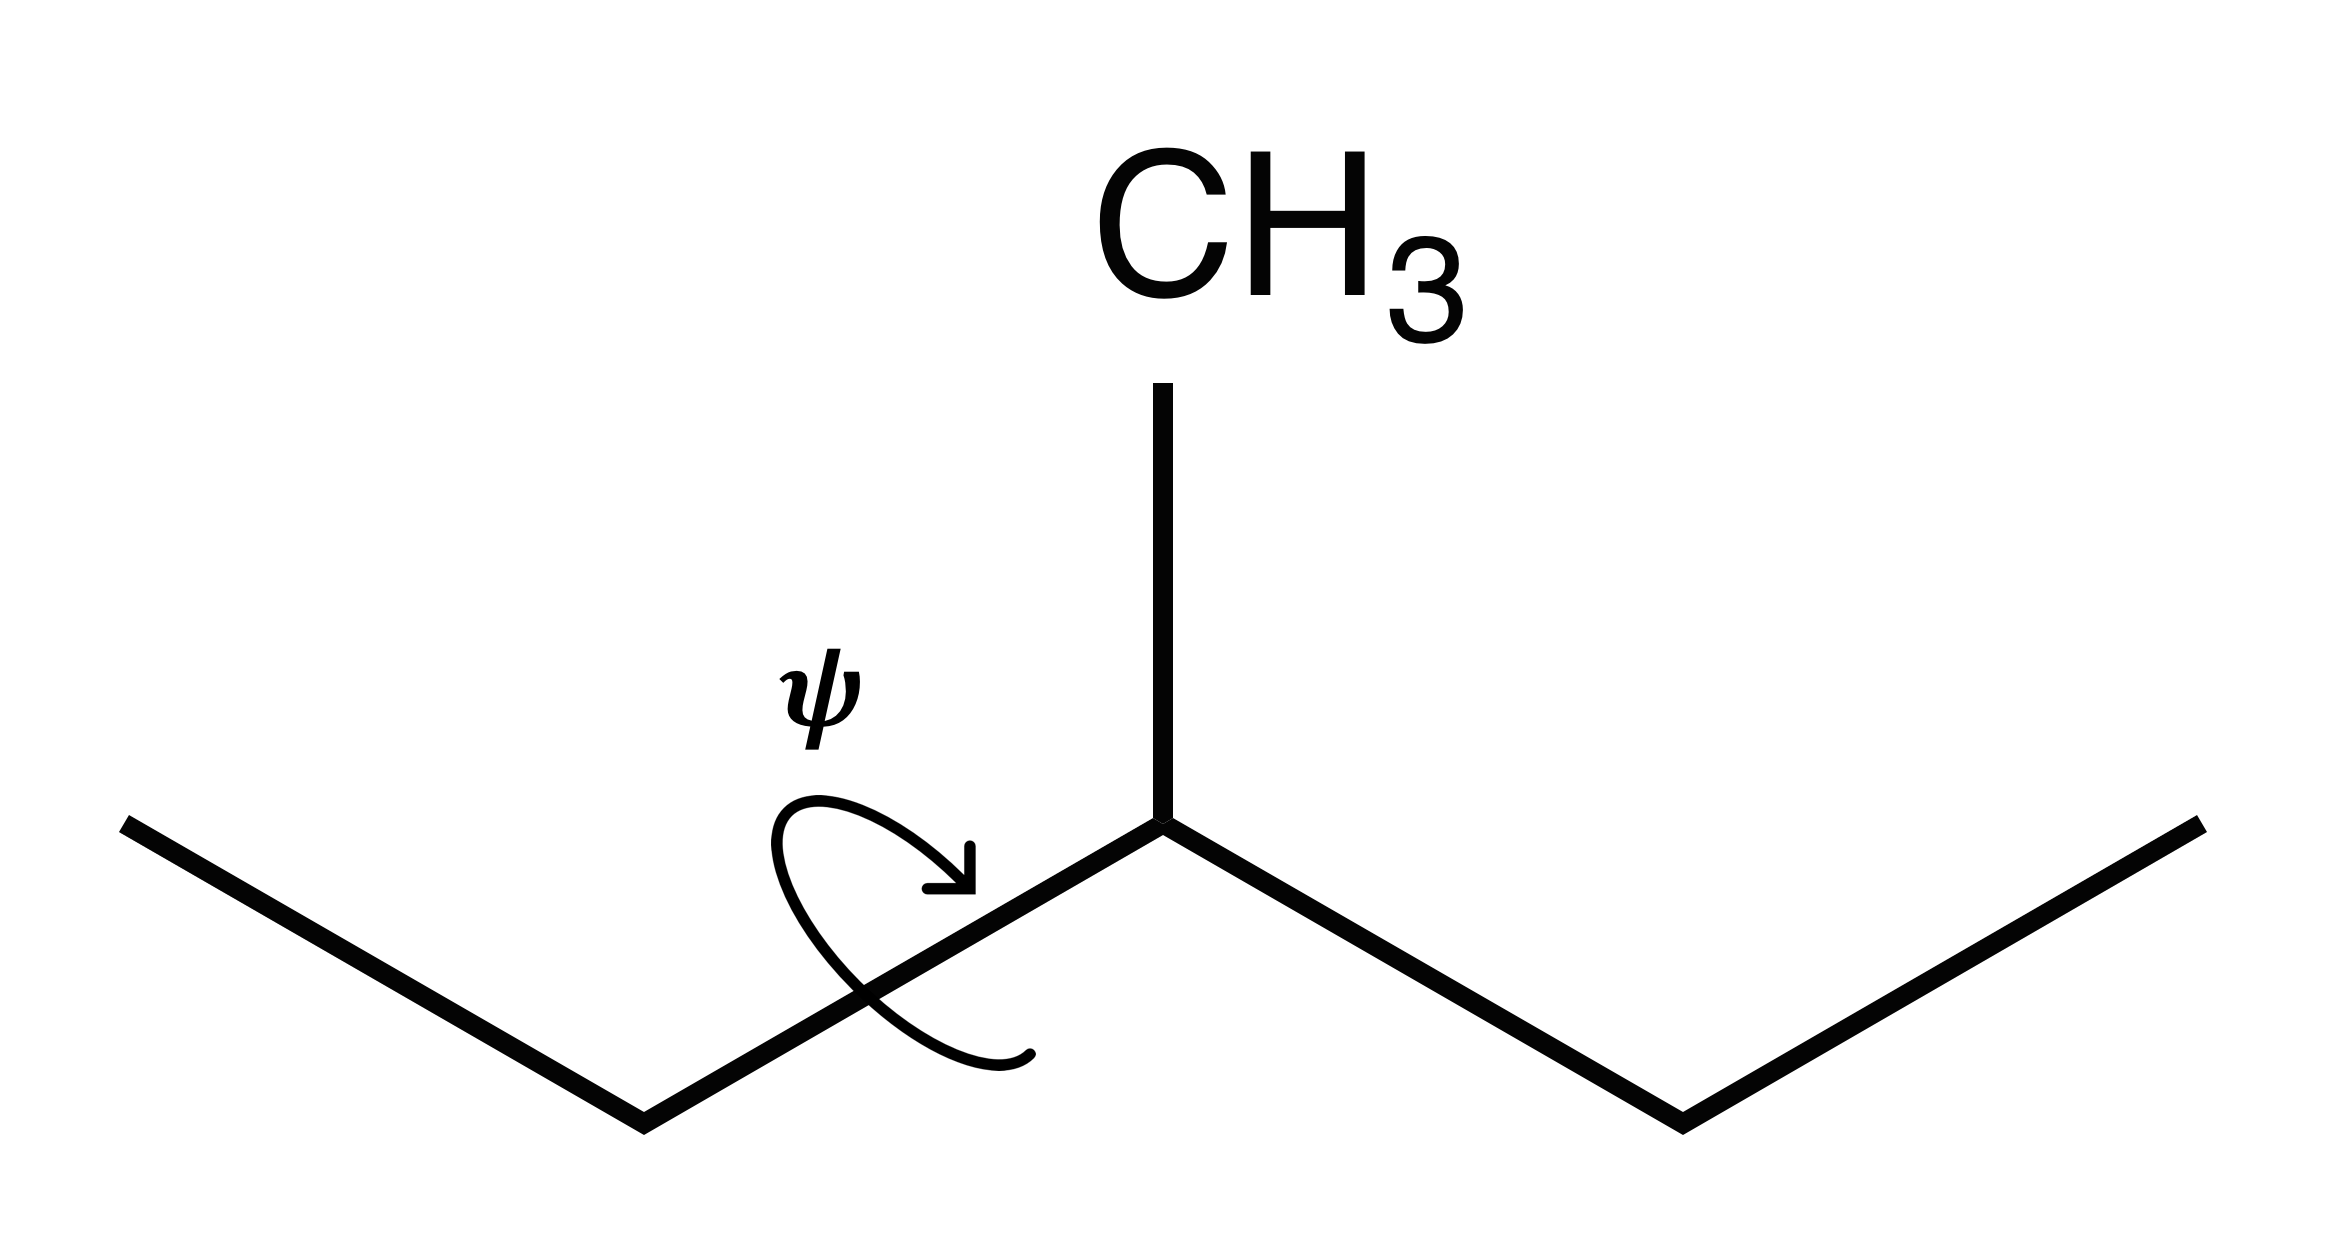
\includegraphics[scale=0.05]{Images/meth0} & 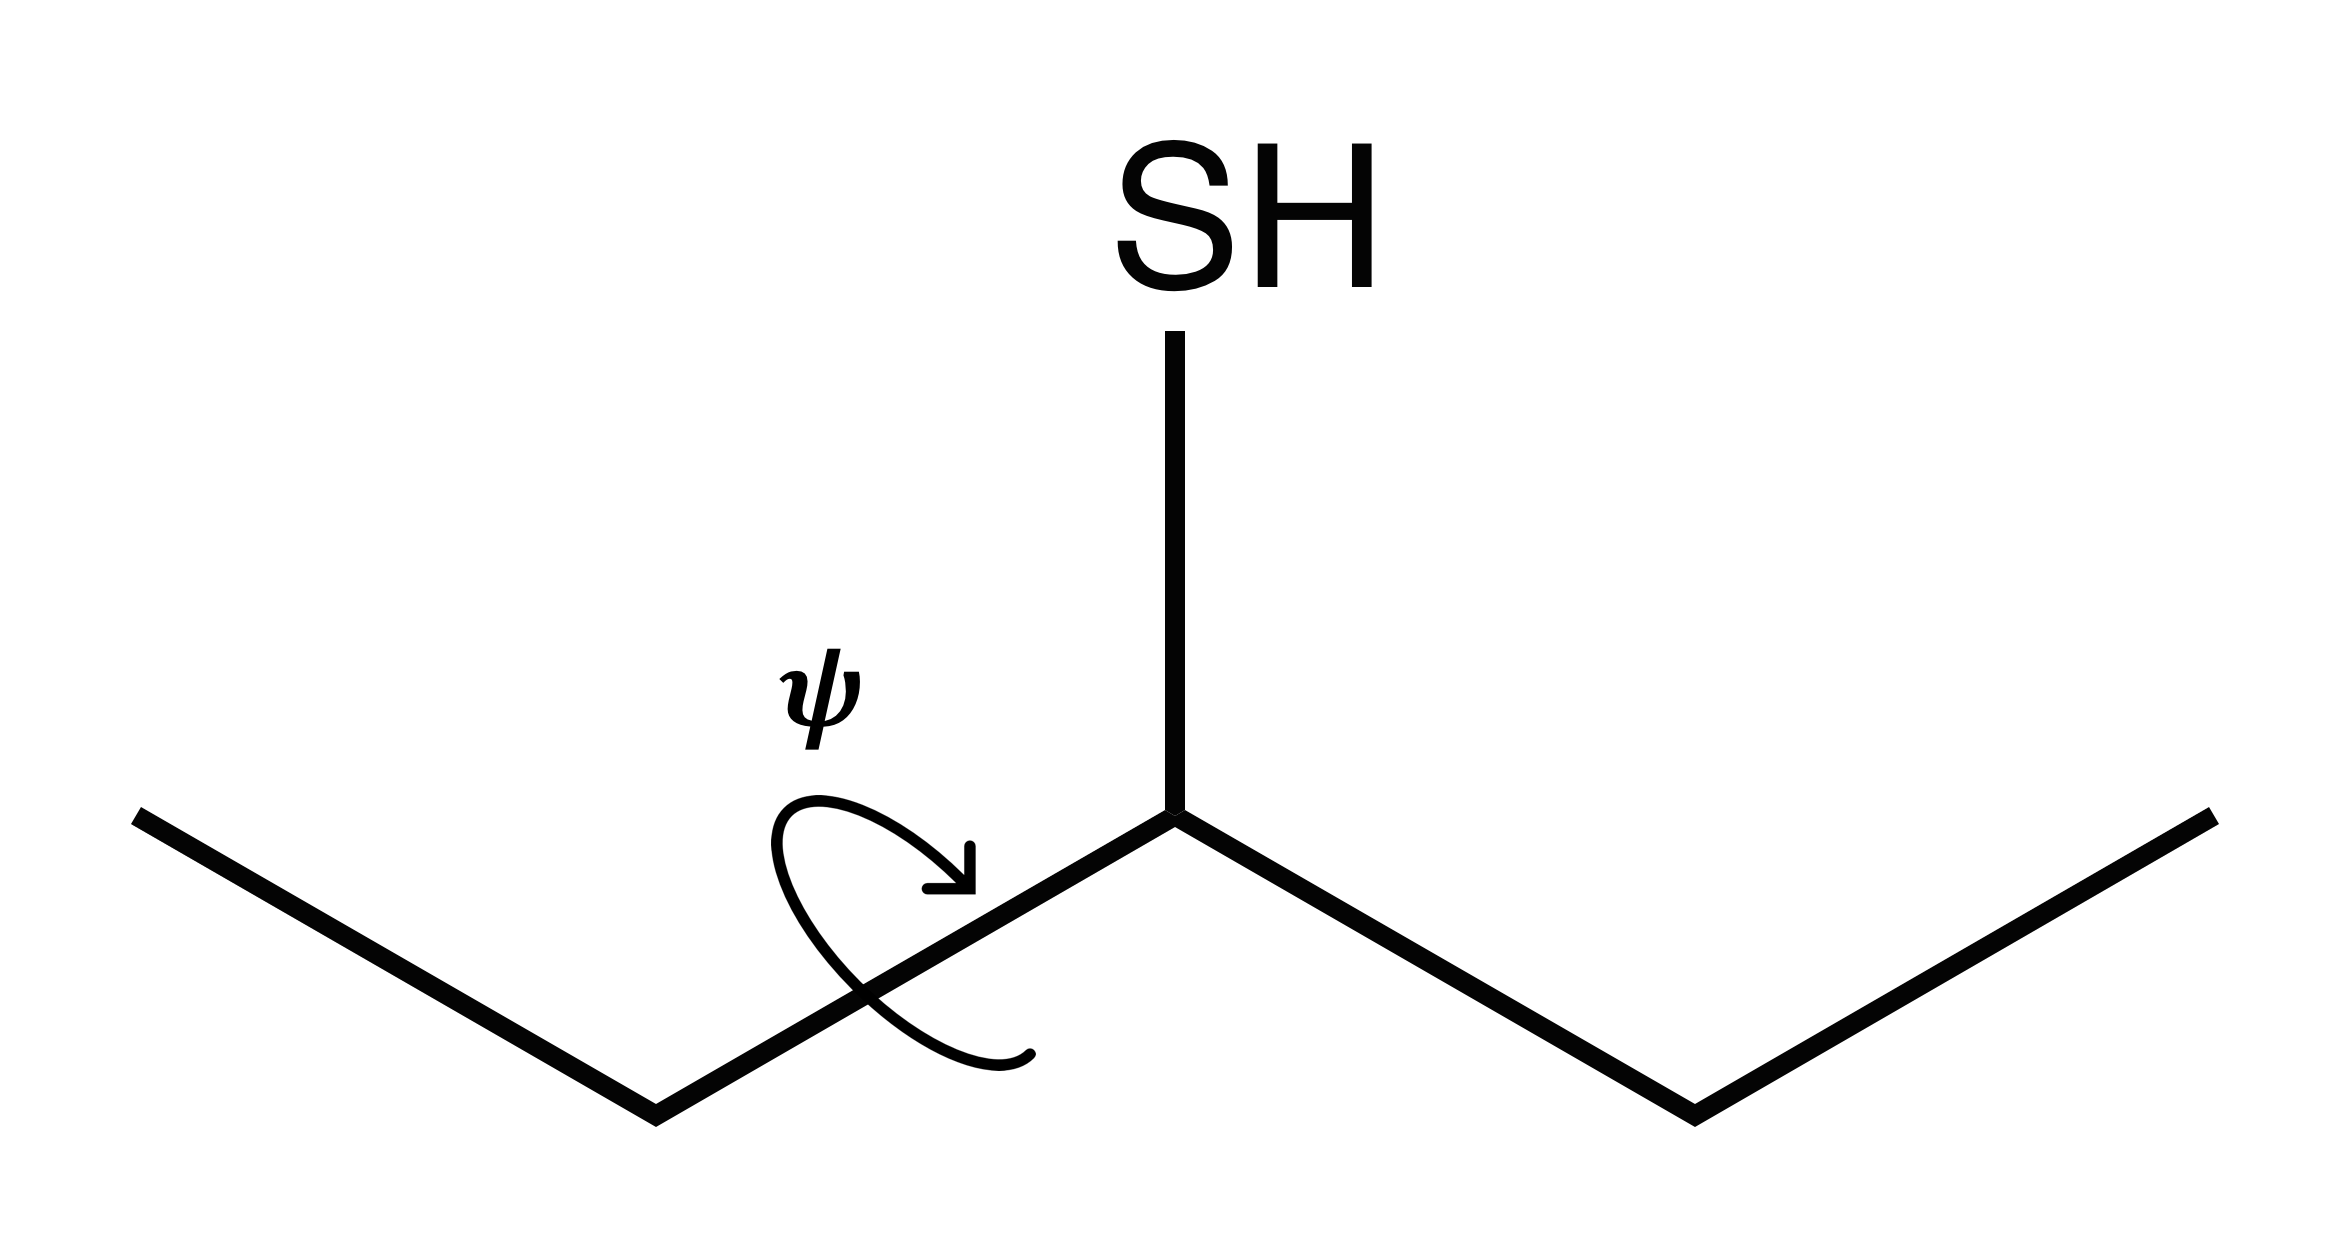
\includegraphics[scale=0.05]{Images/thio0} \\
 & 26640 & 26643 & 847 & 756 & 26650 \\ \hline
\multirow{2}{*}{1} & 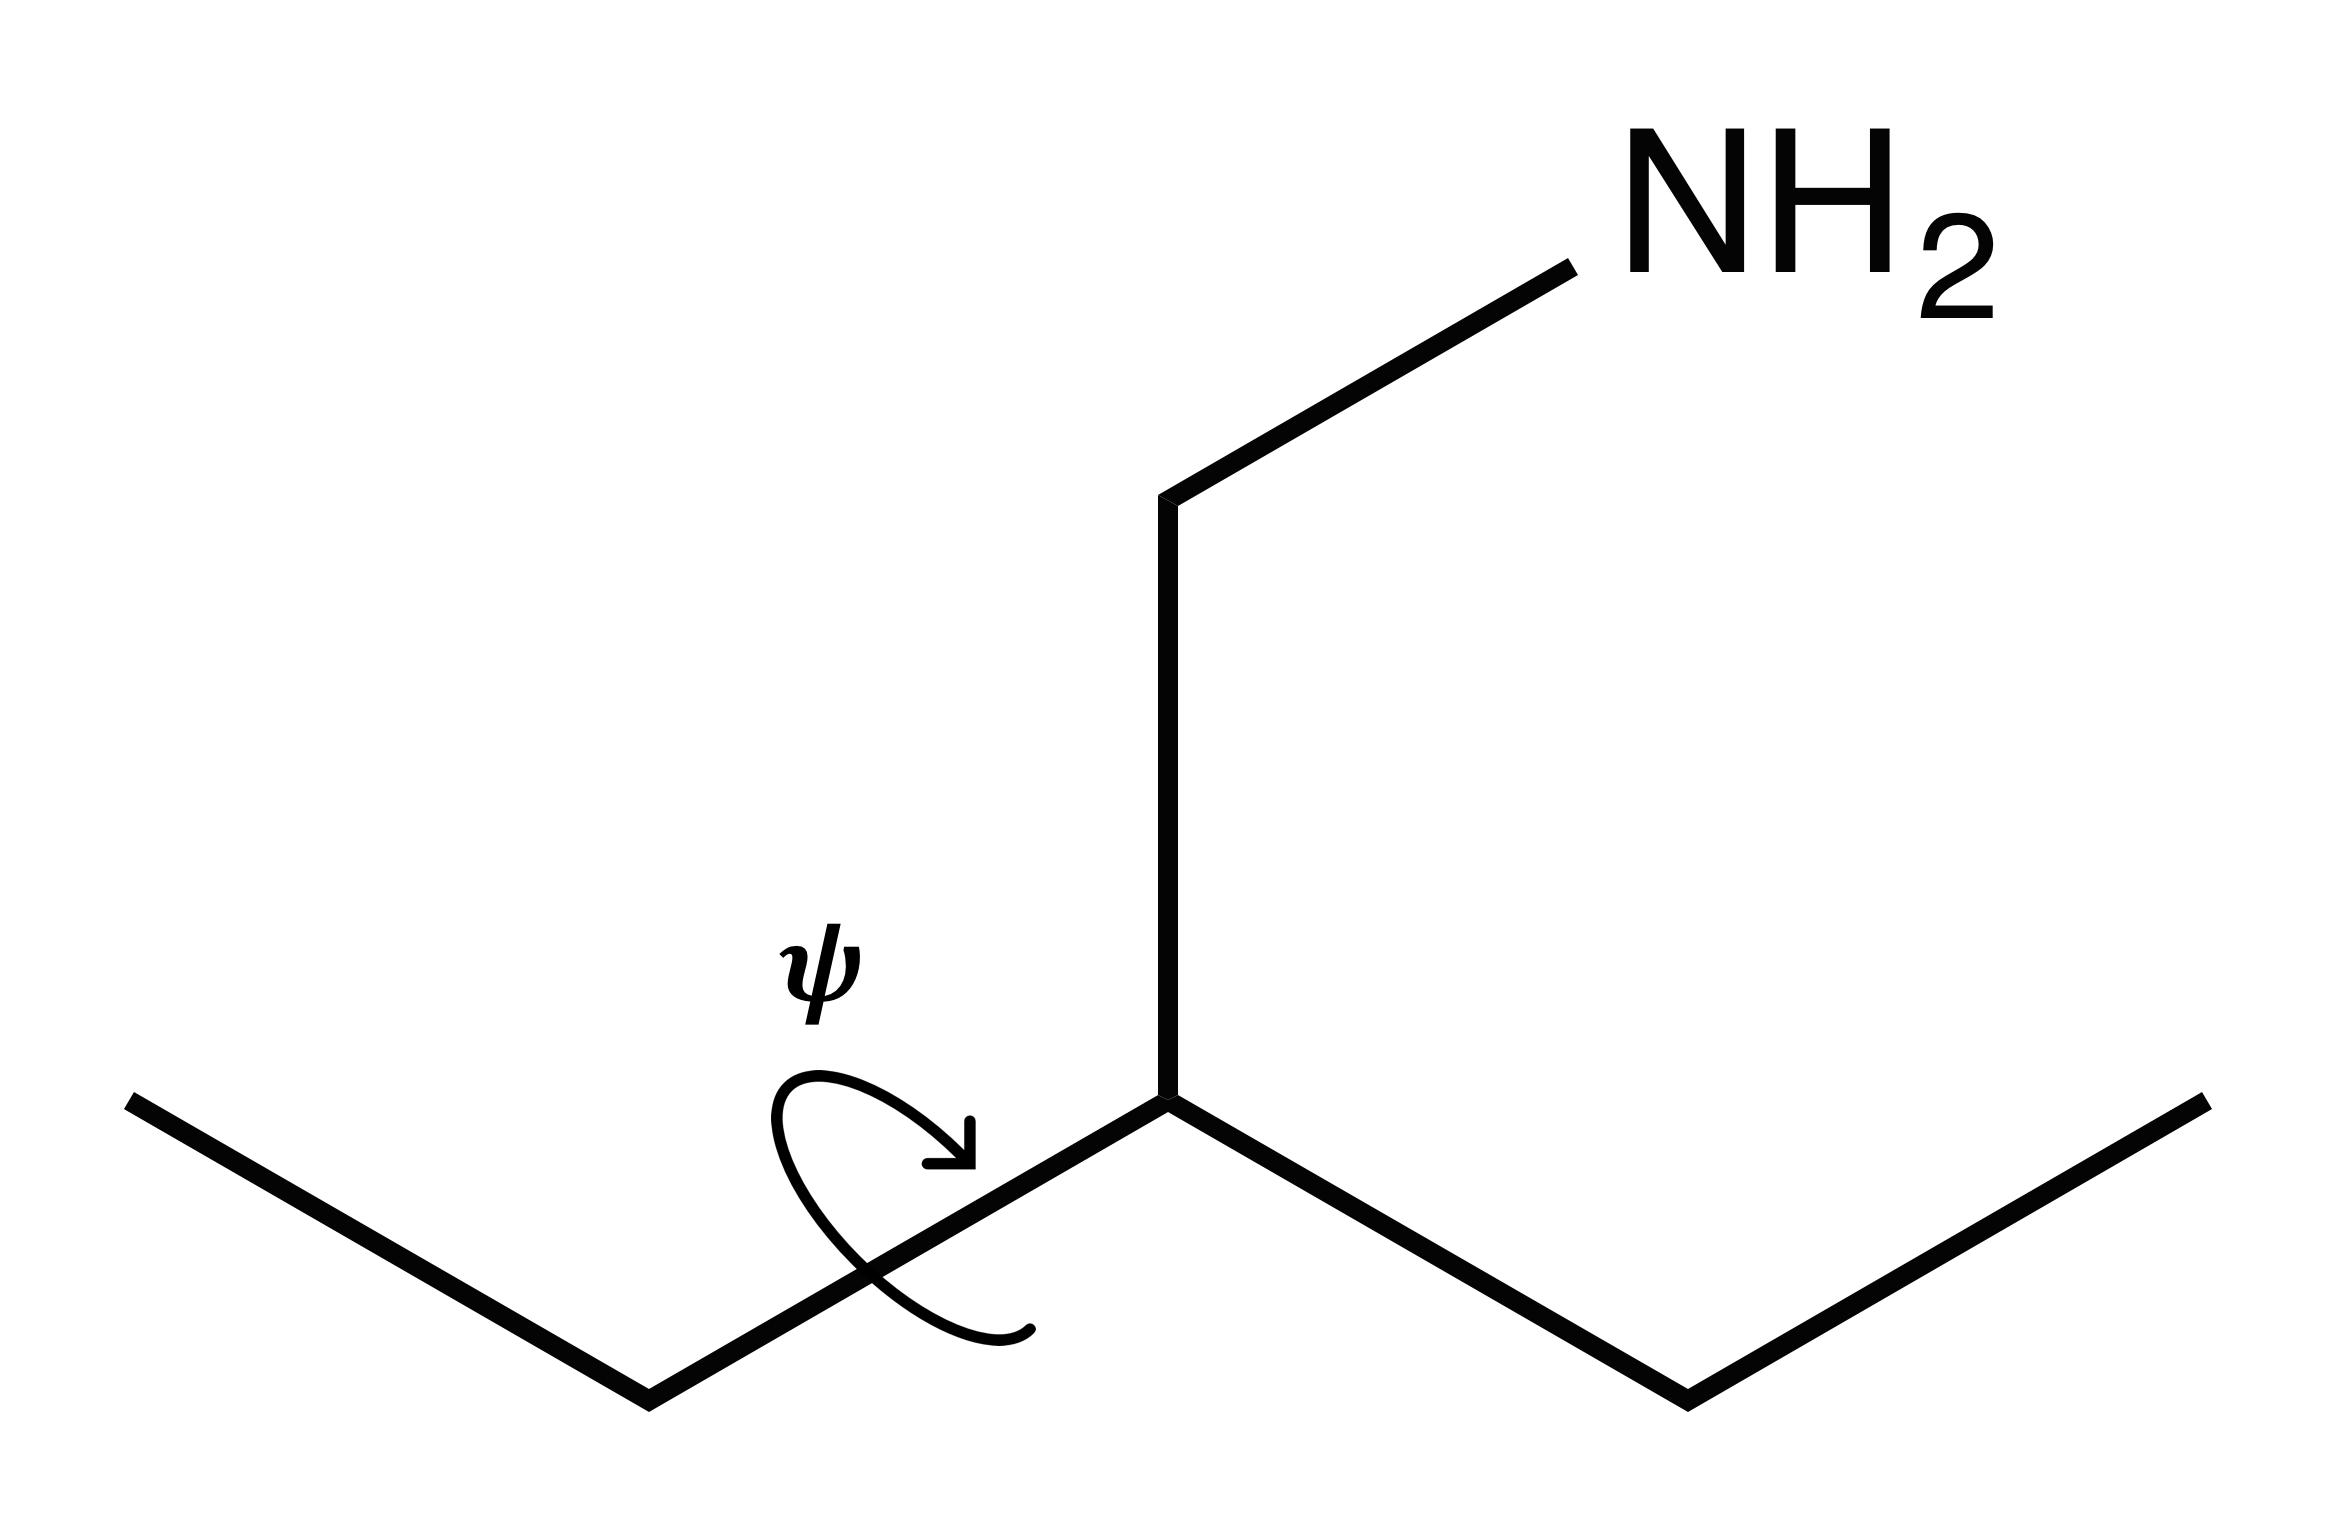
\includegraphics[scale=0.05]{Images/amino1} & 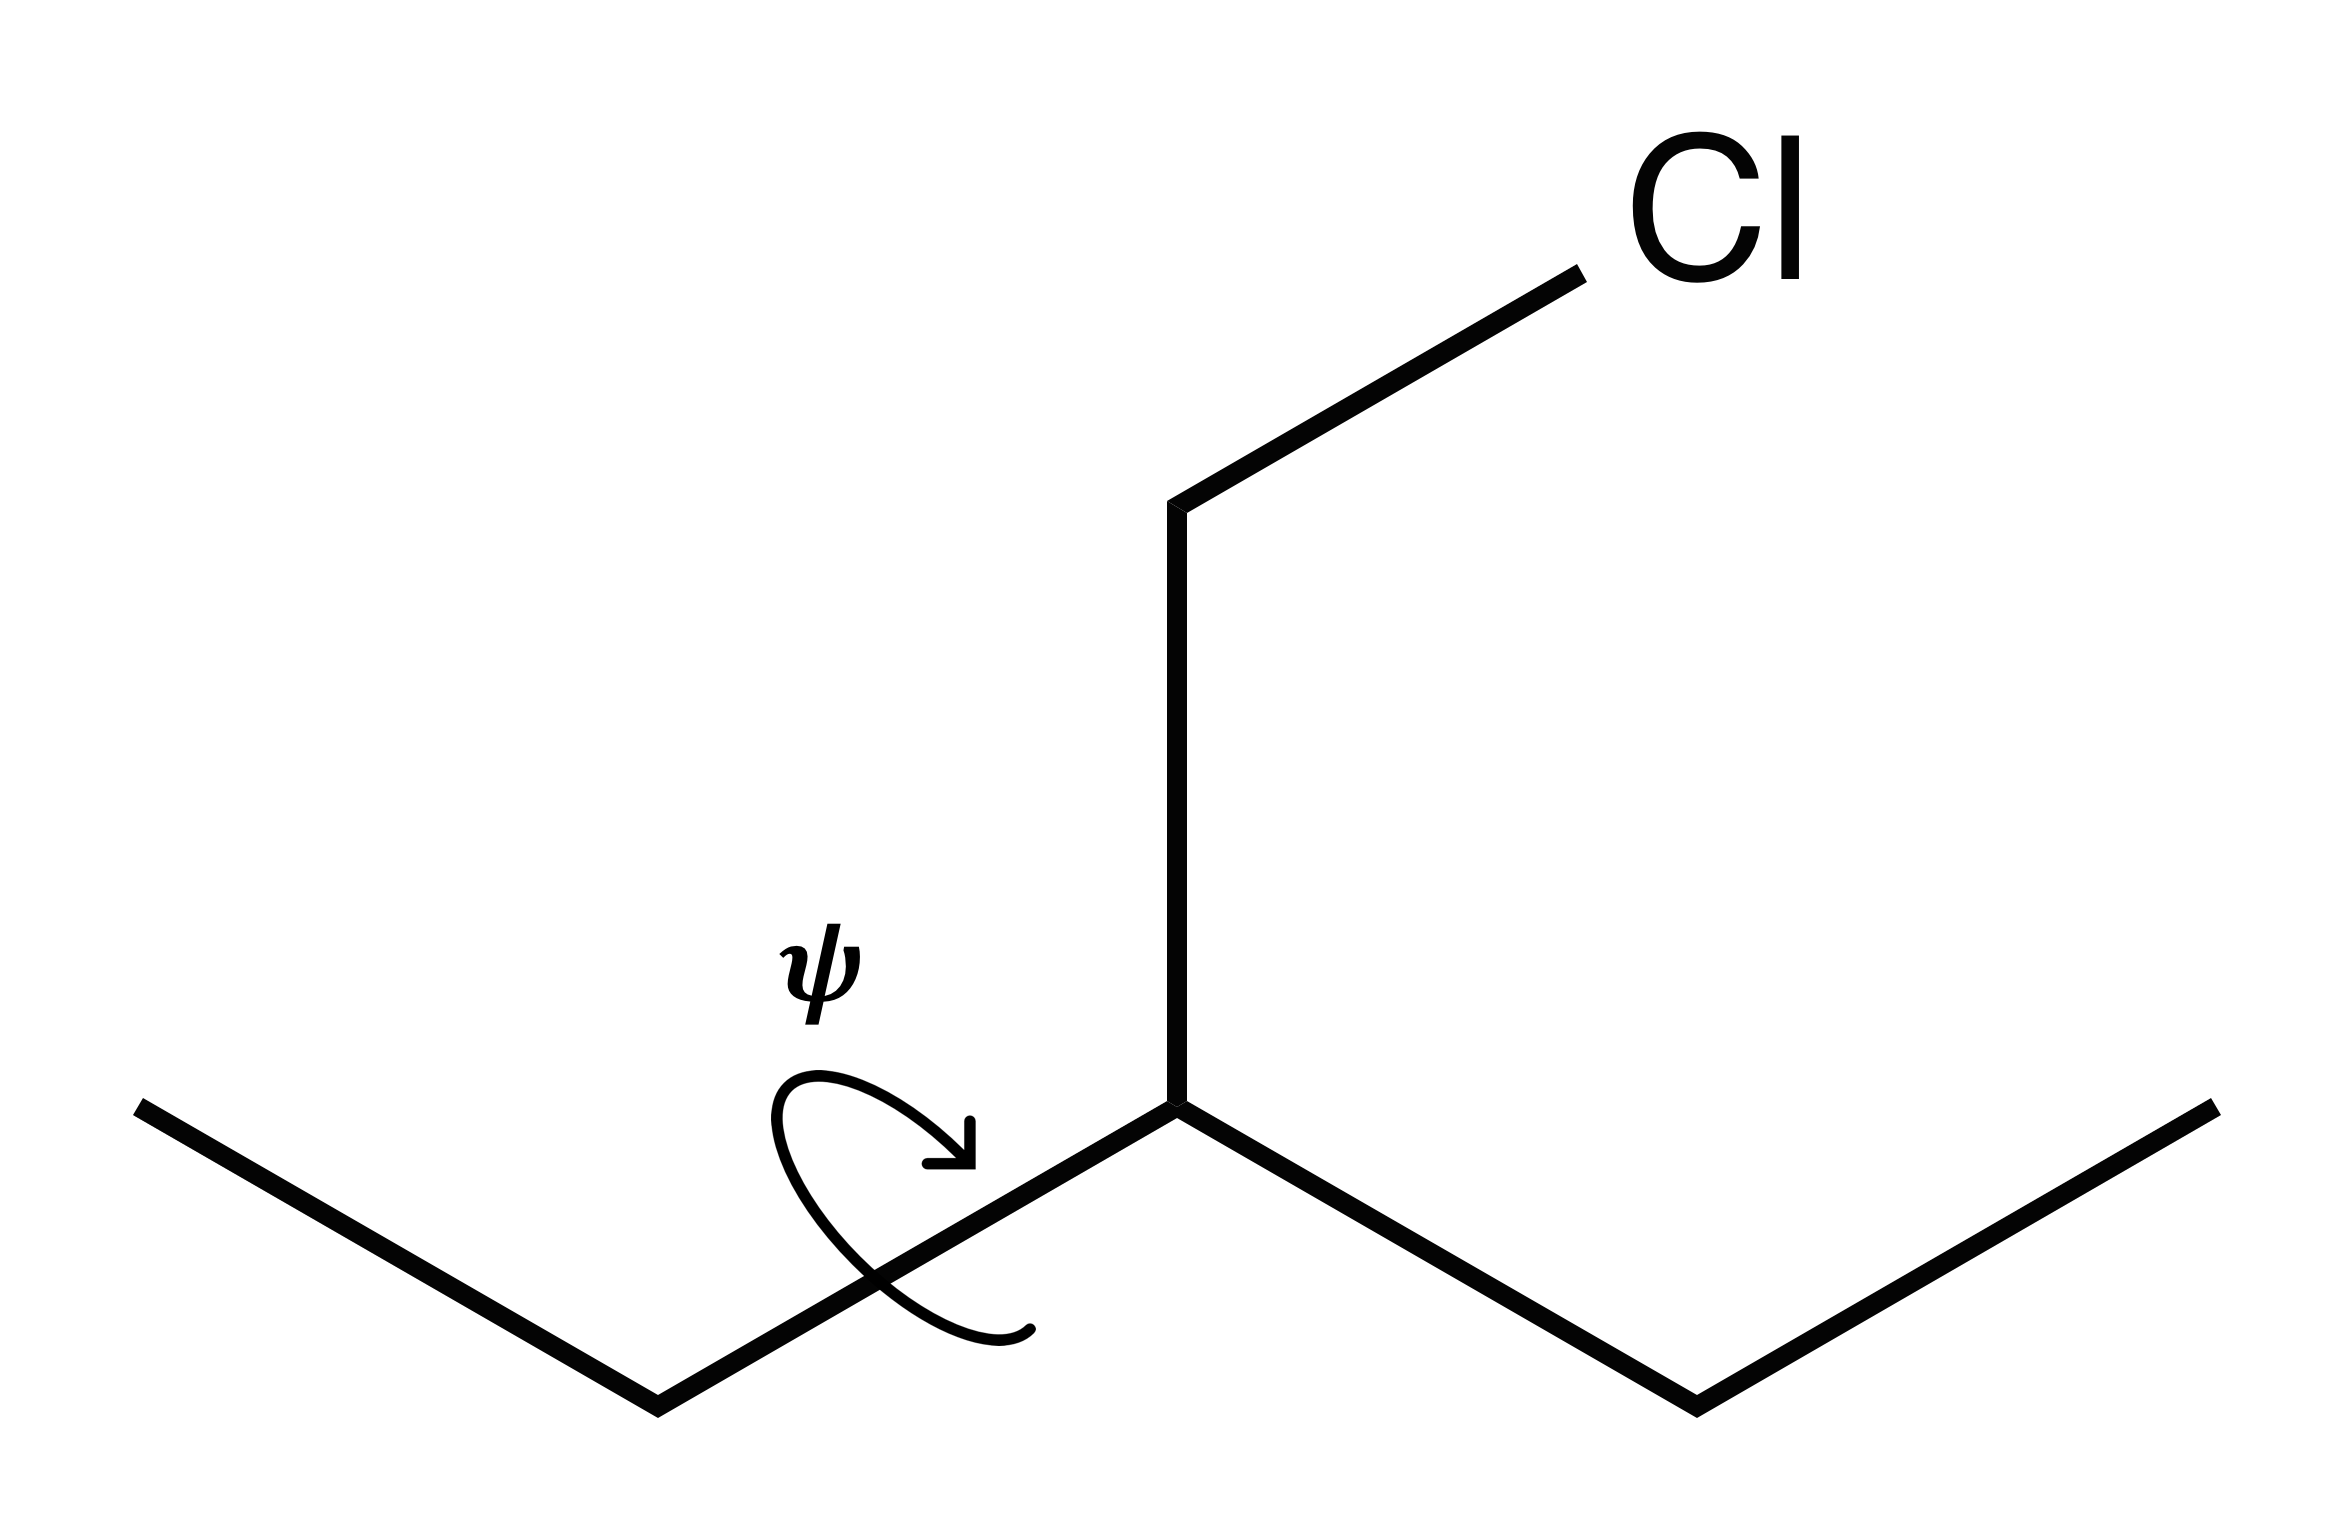
\includegraphics[scale=0.05]{Images/chloro1} & 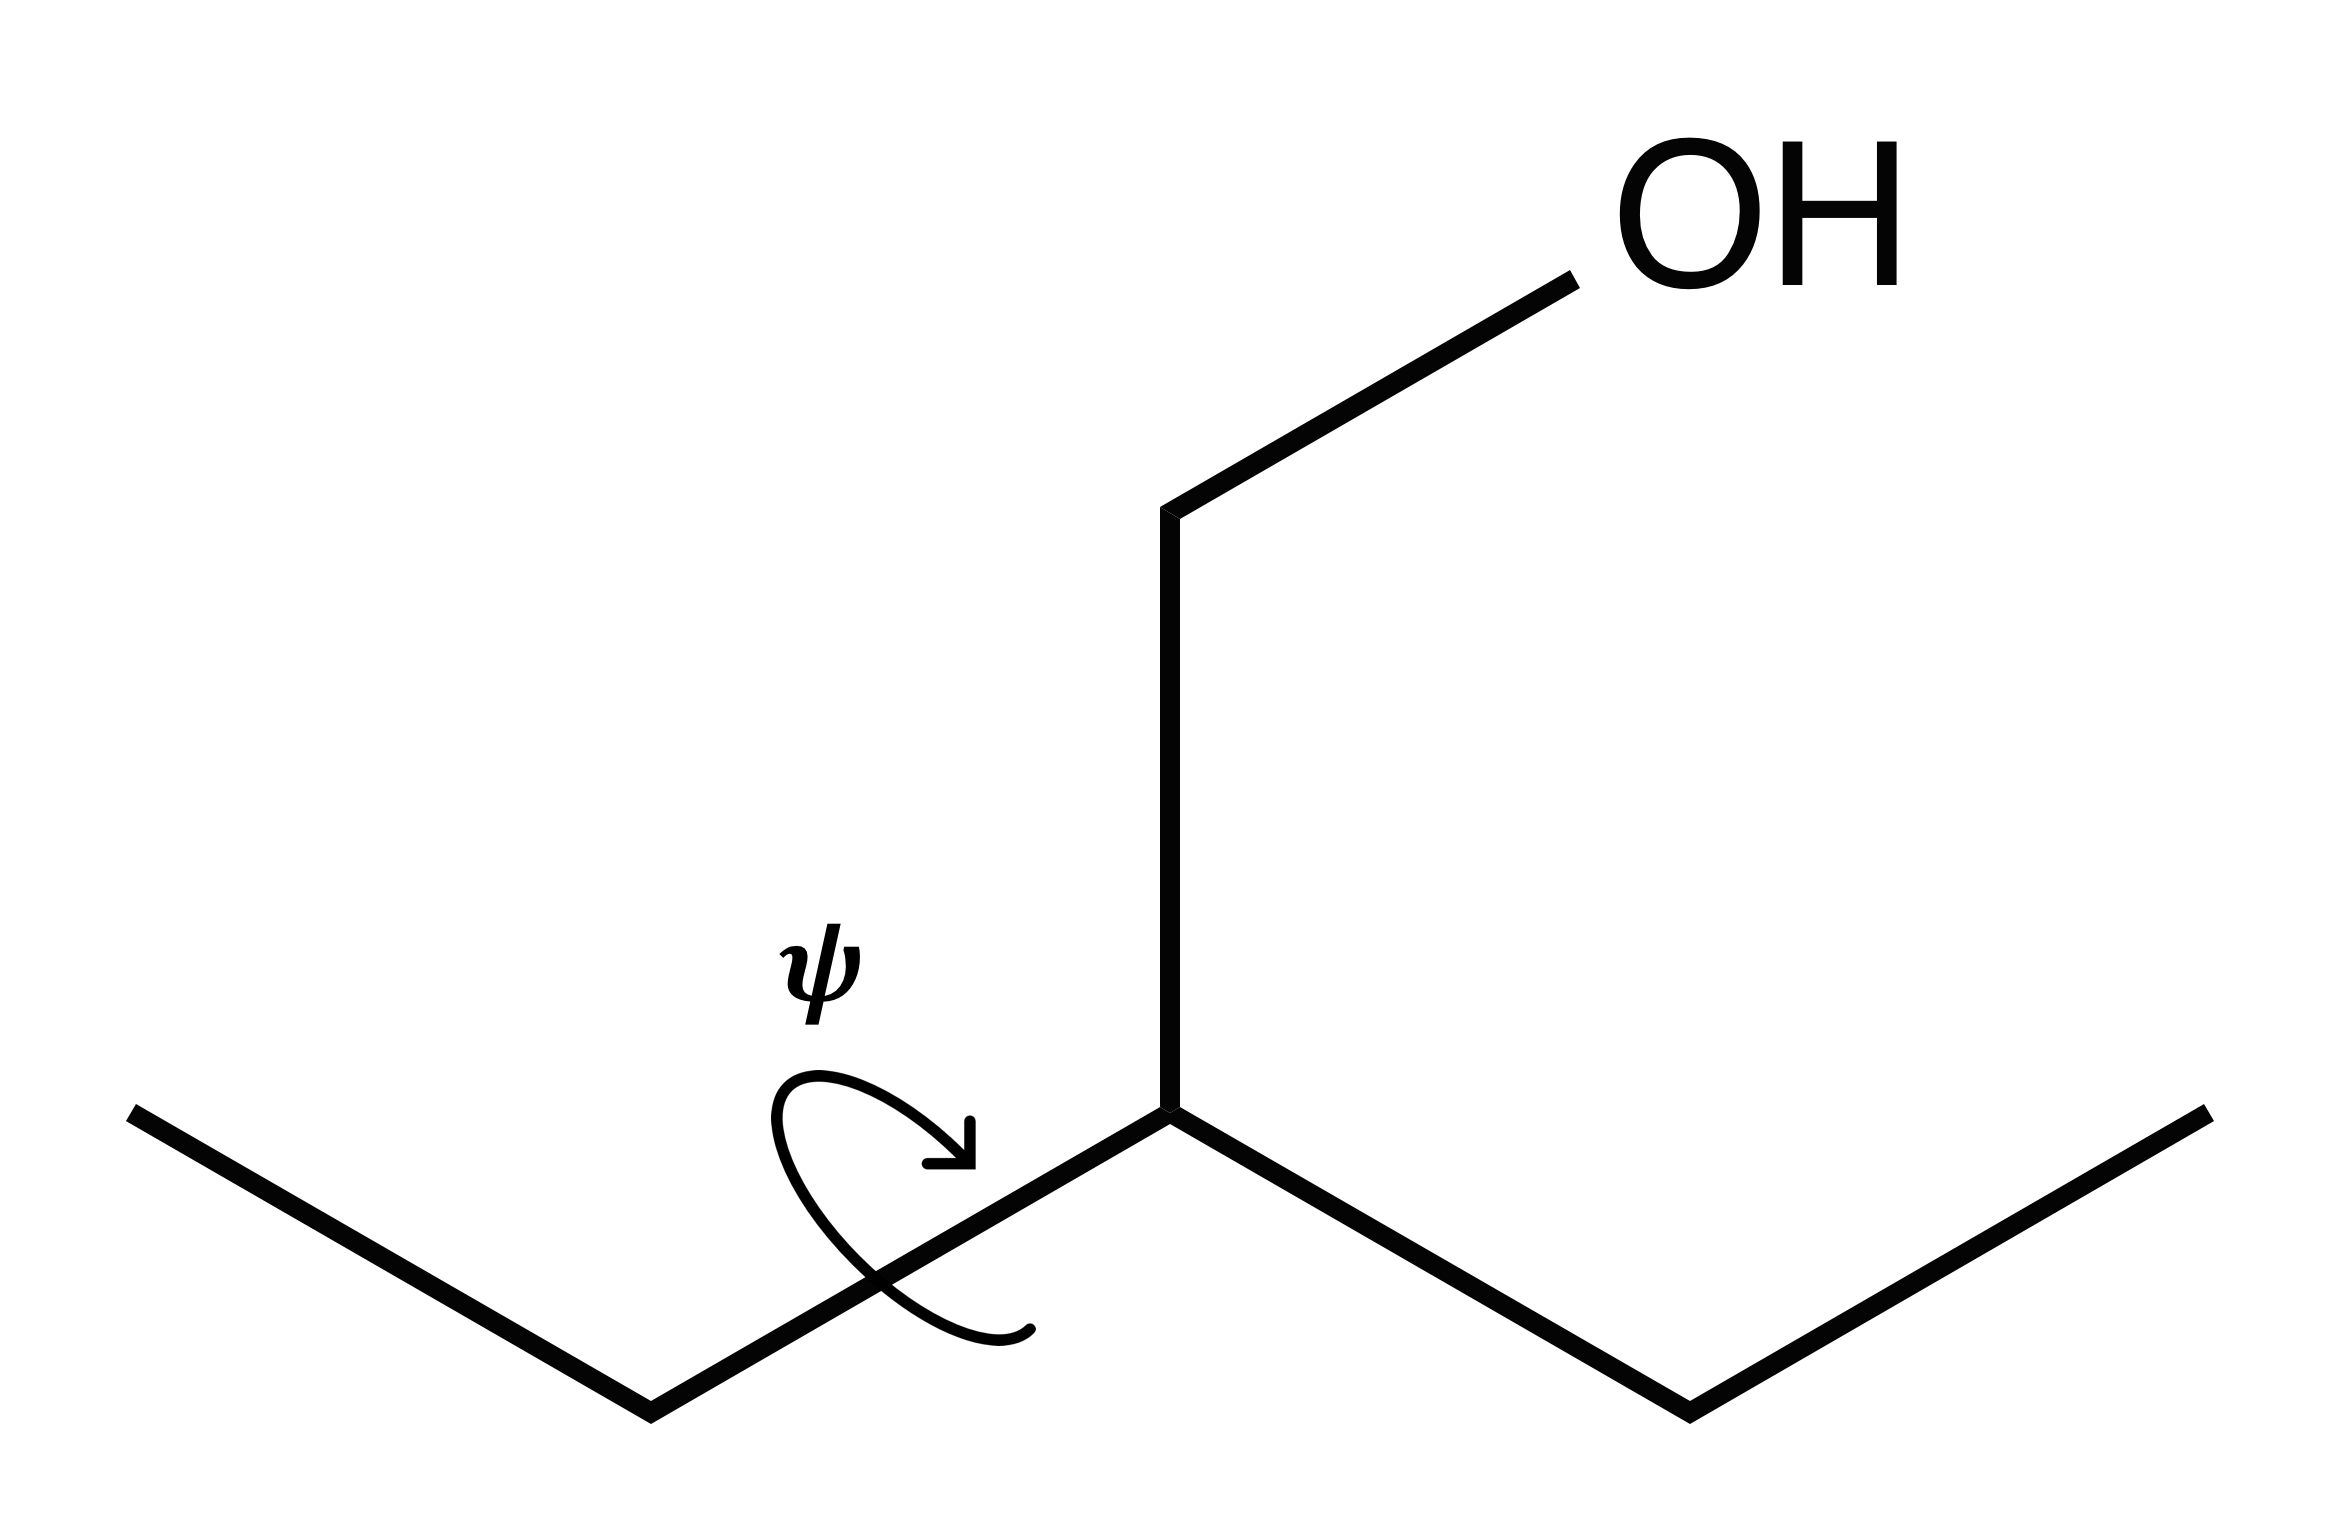
\includegraphics[scale=0.05]{Images/hydro1} & 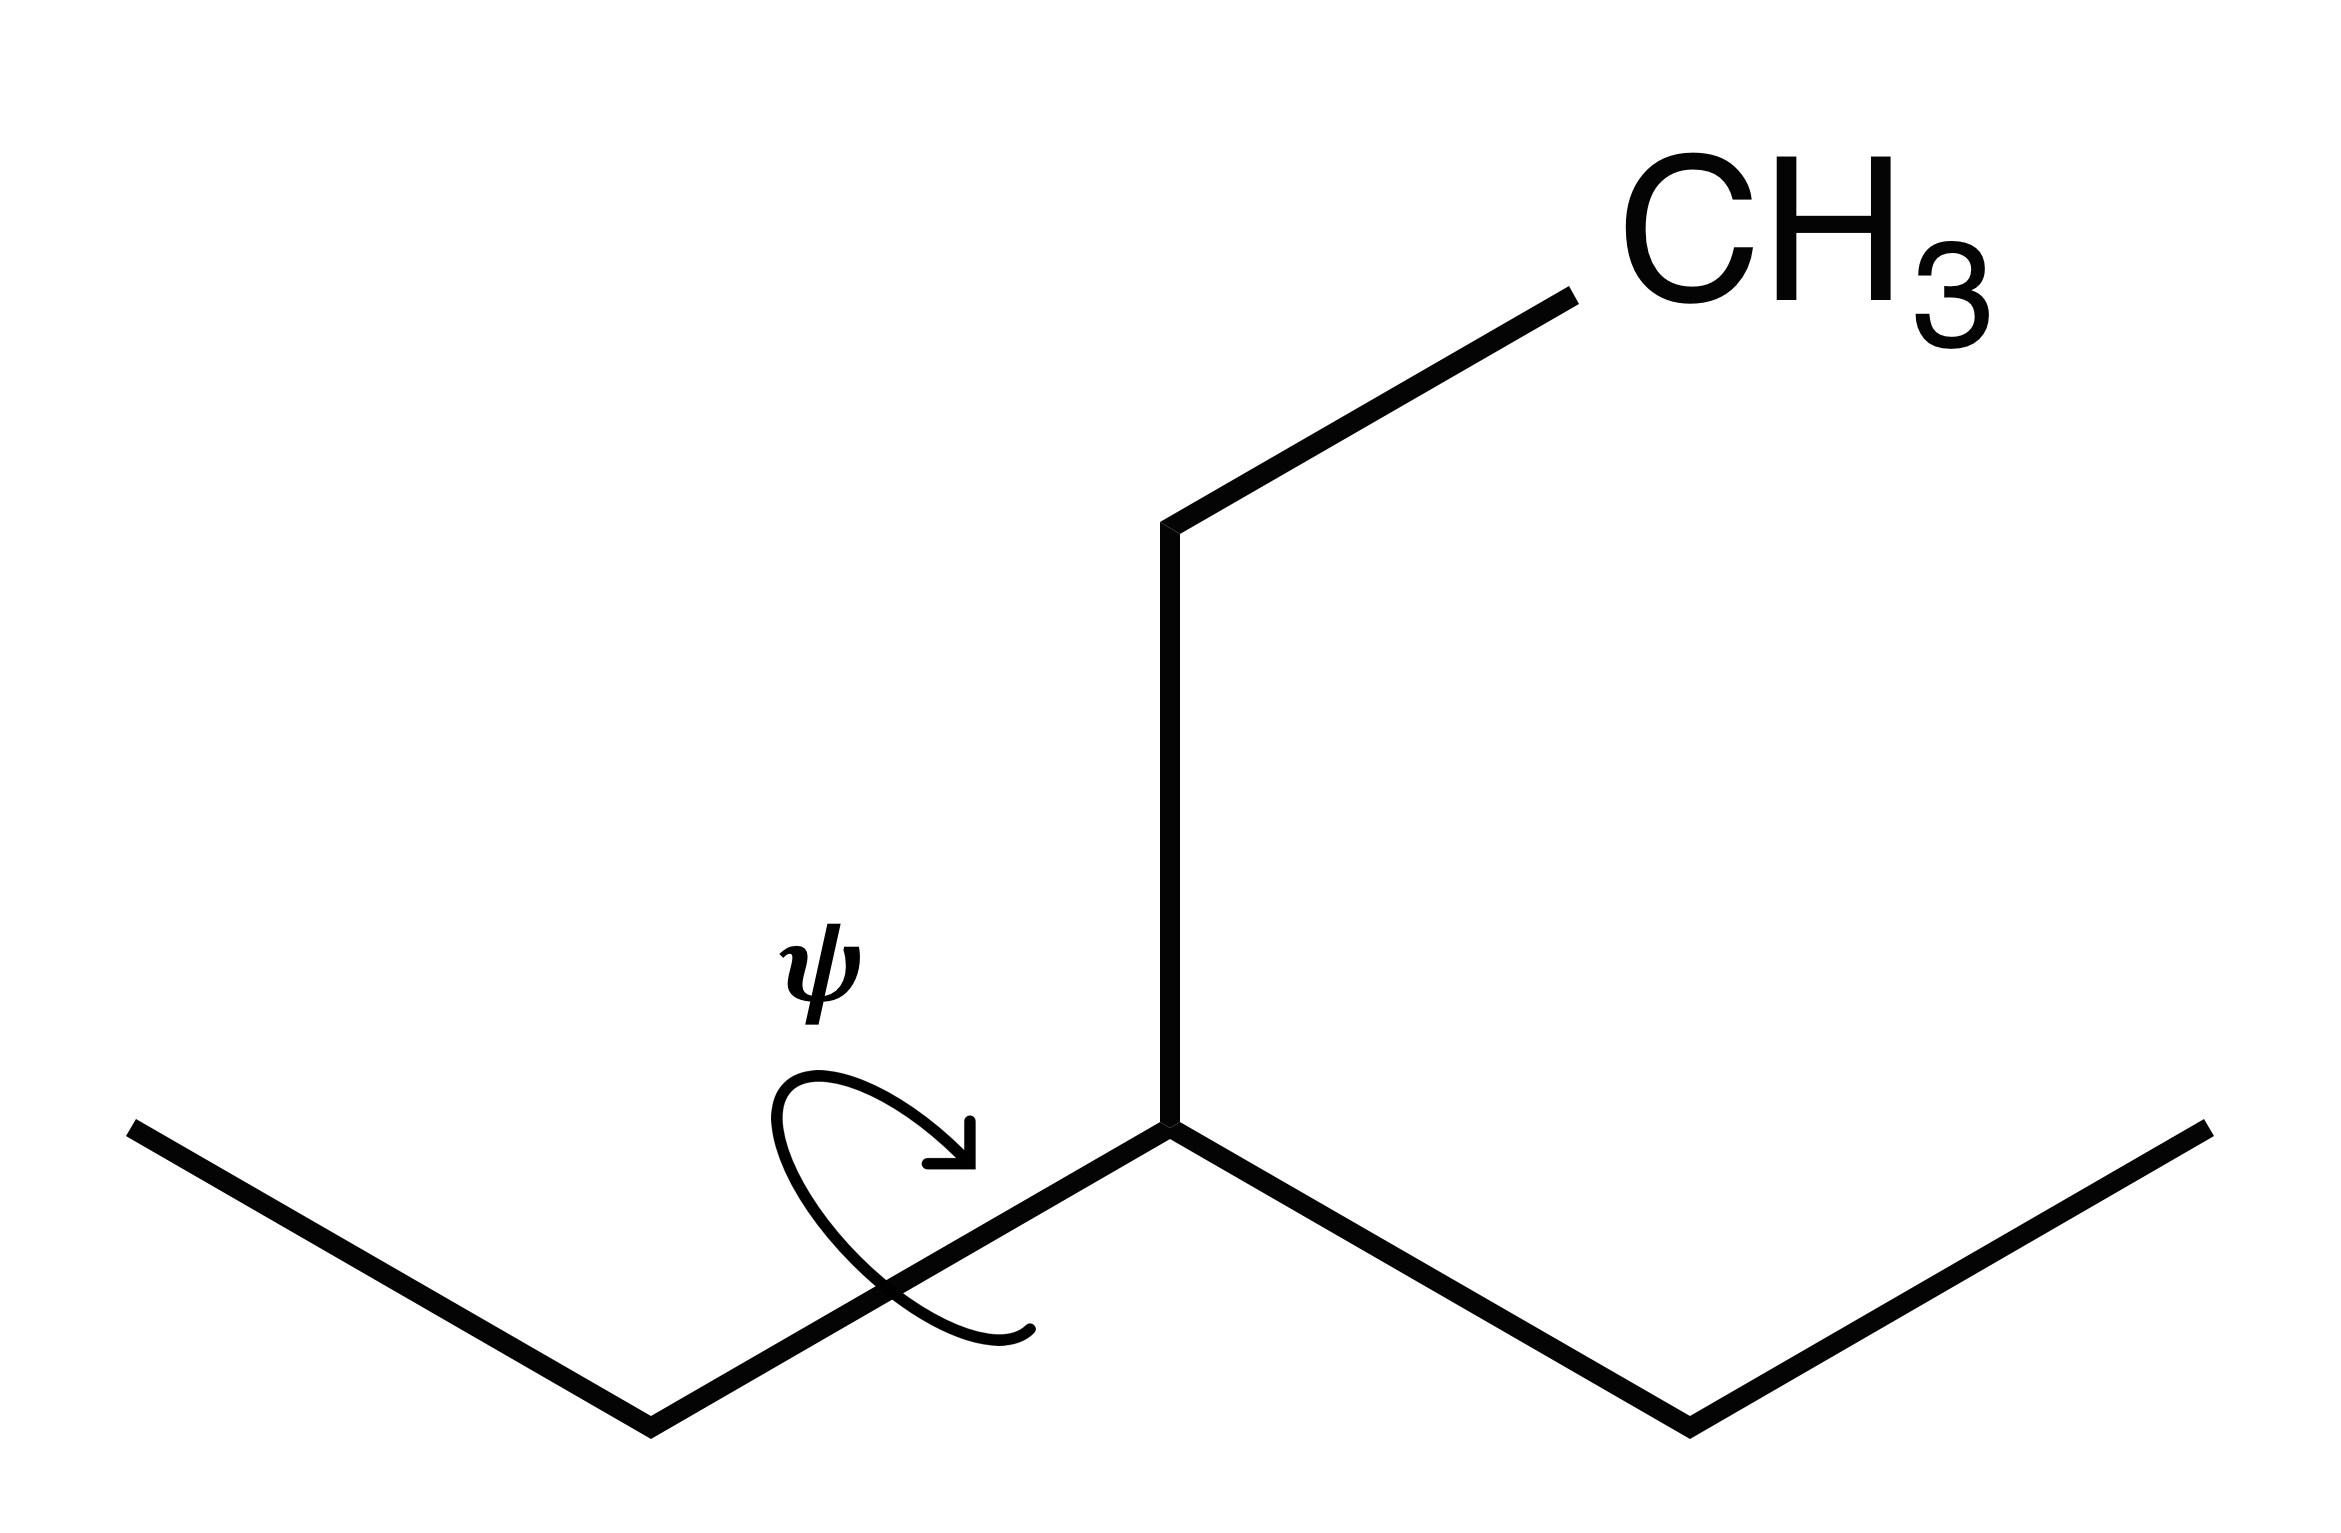
\includegraphics[scale=0.05]{Images/meth1} & 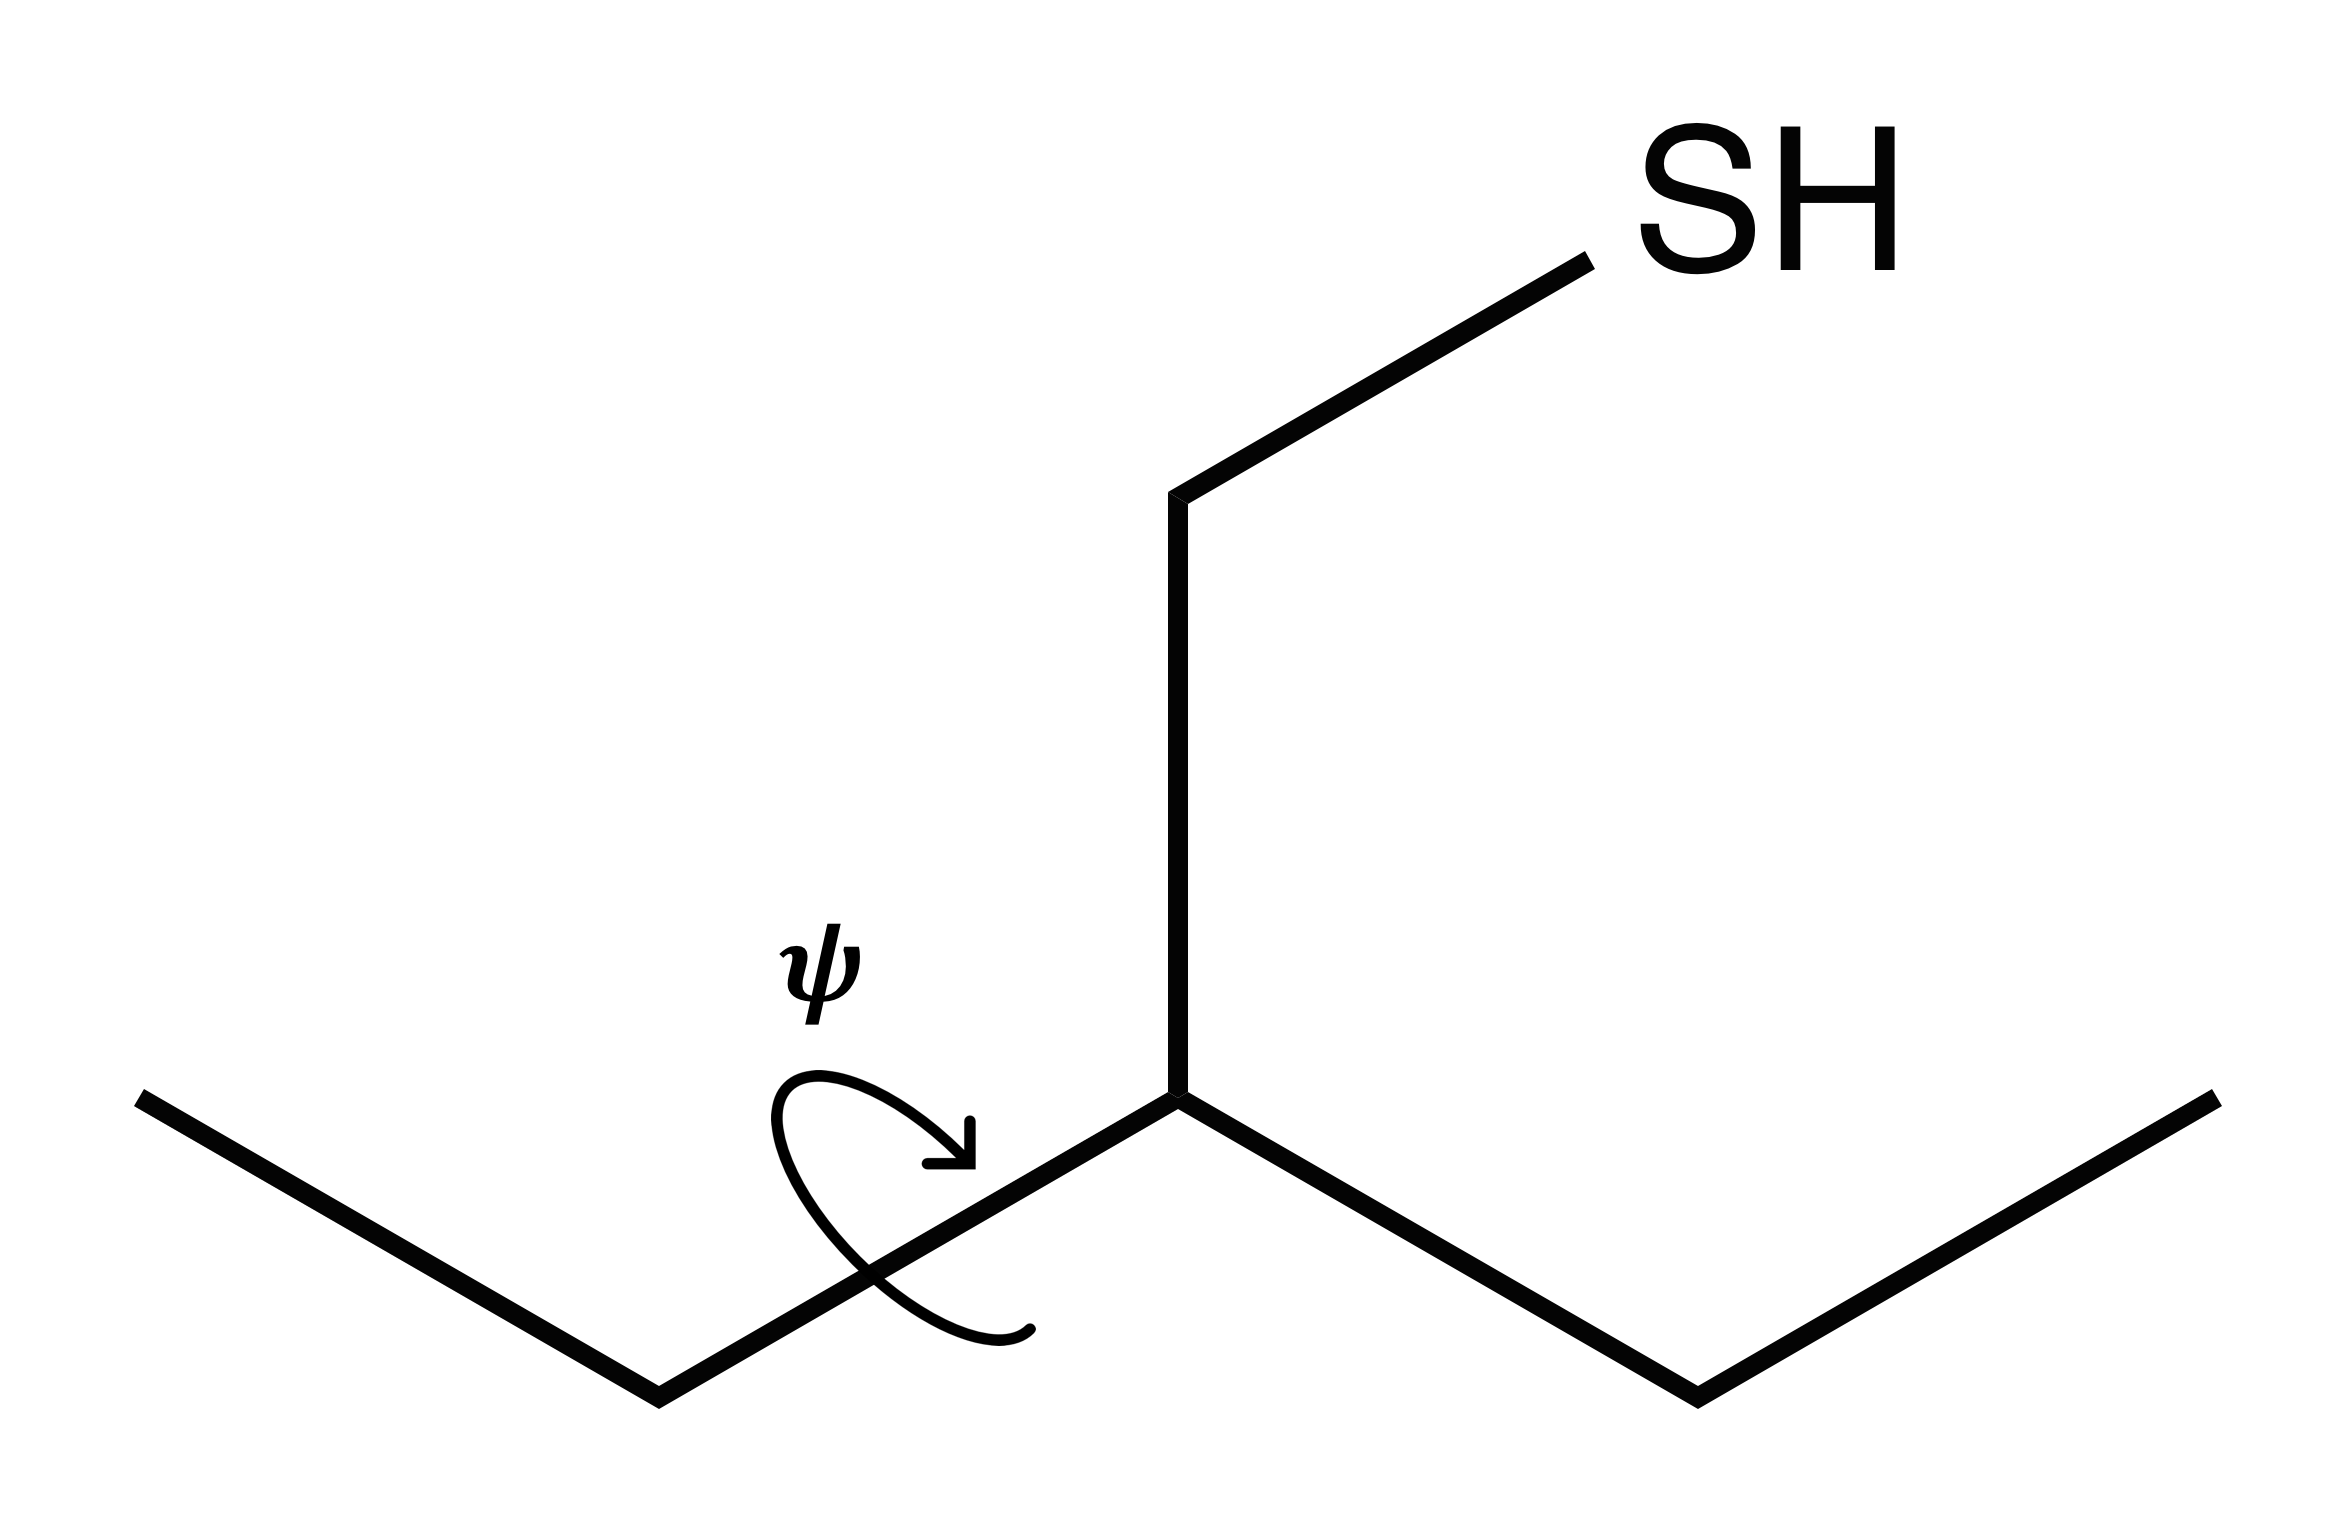
\includegraphics[scale=0.05]{Images/thio1} \\
 & 26641 & 26644 & 26646 & 26648 & 26651 \\ \hline
\multirow{2}{*}{2} & 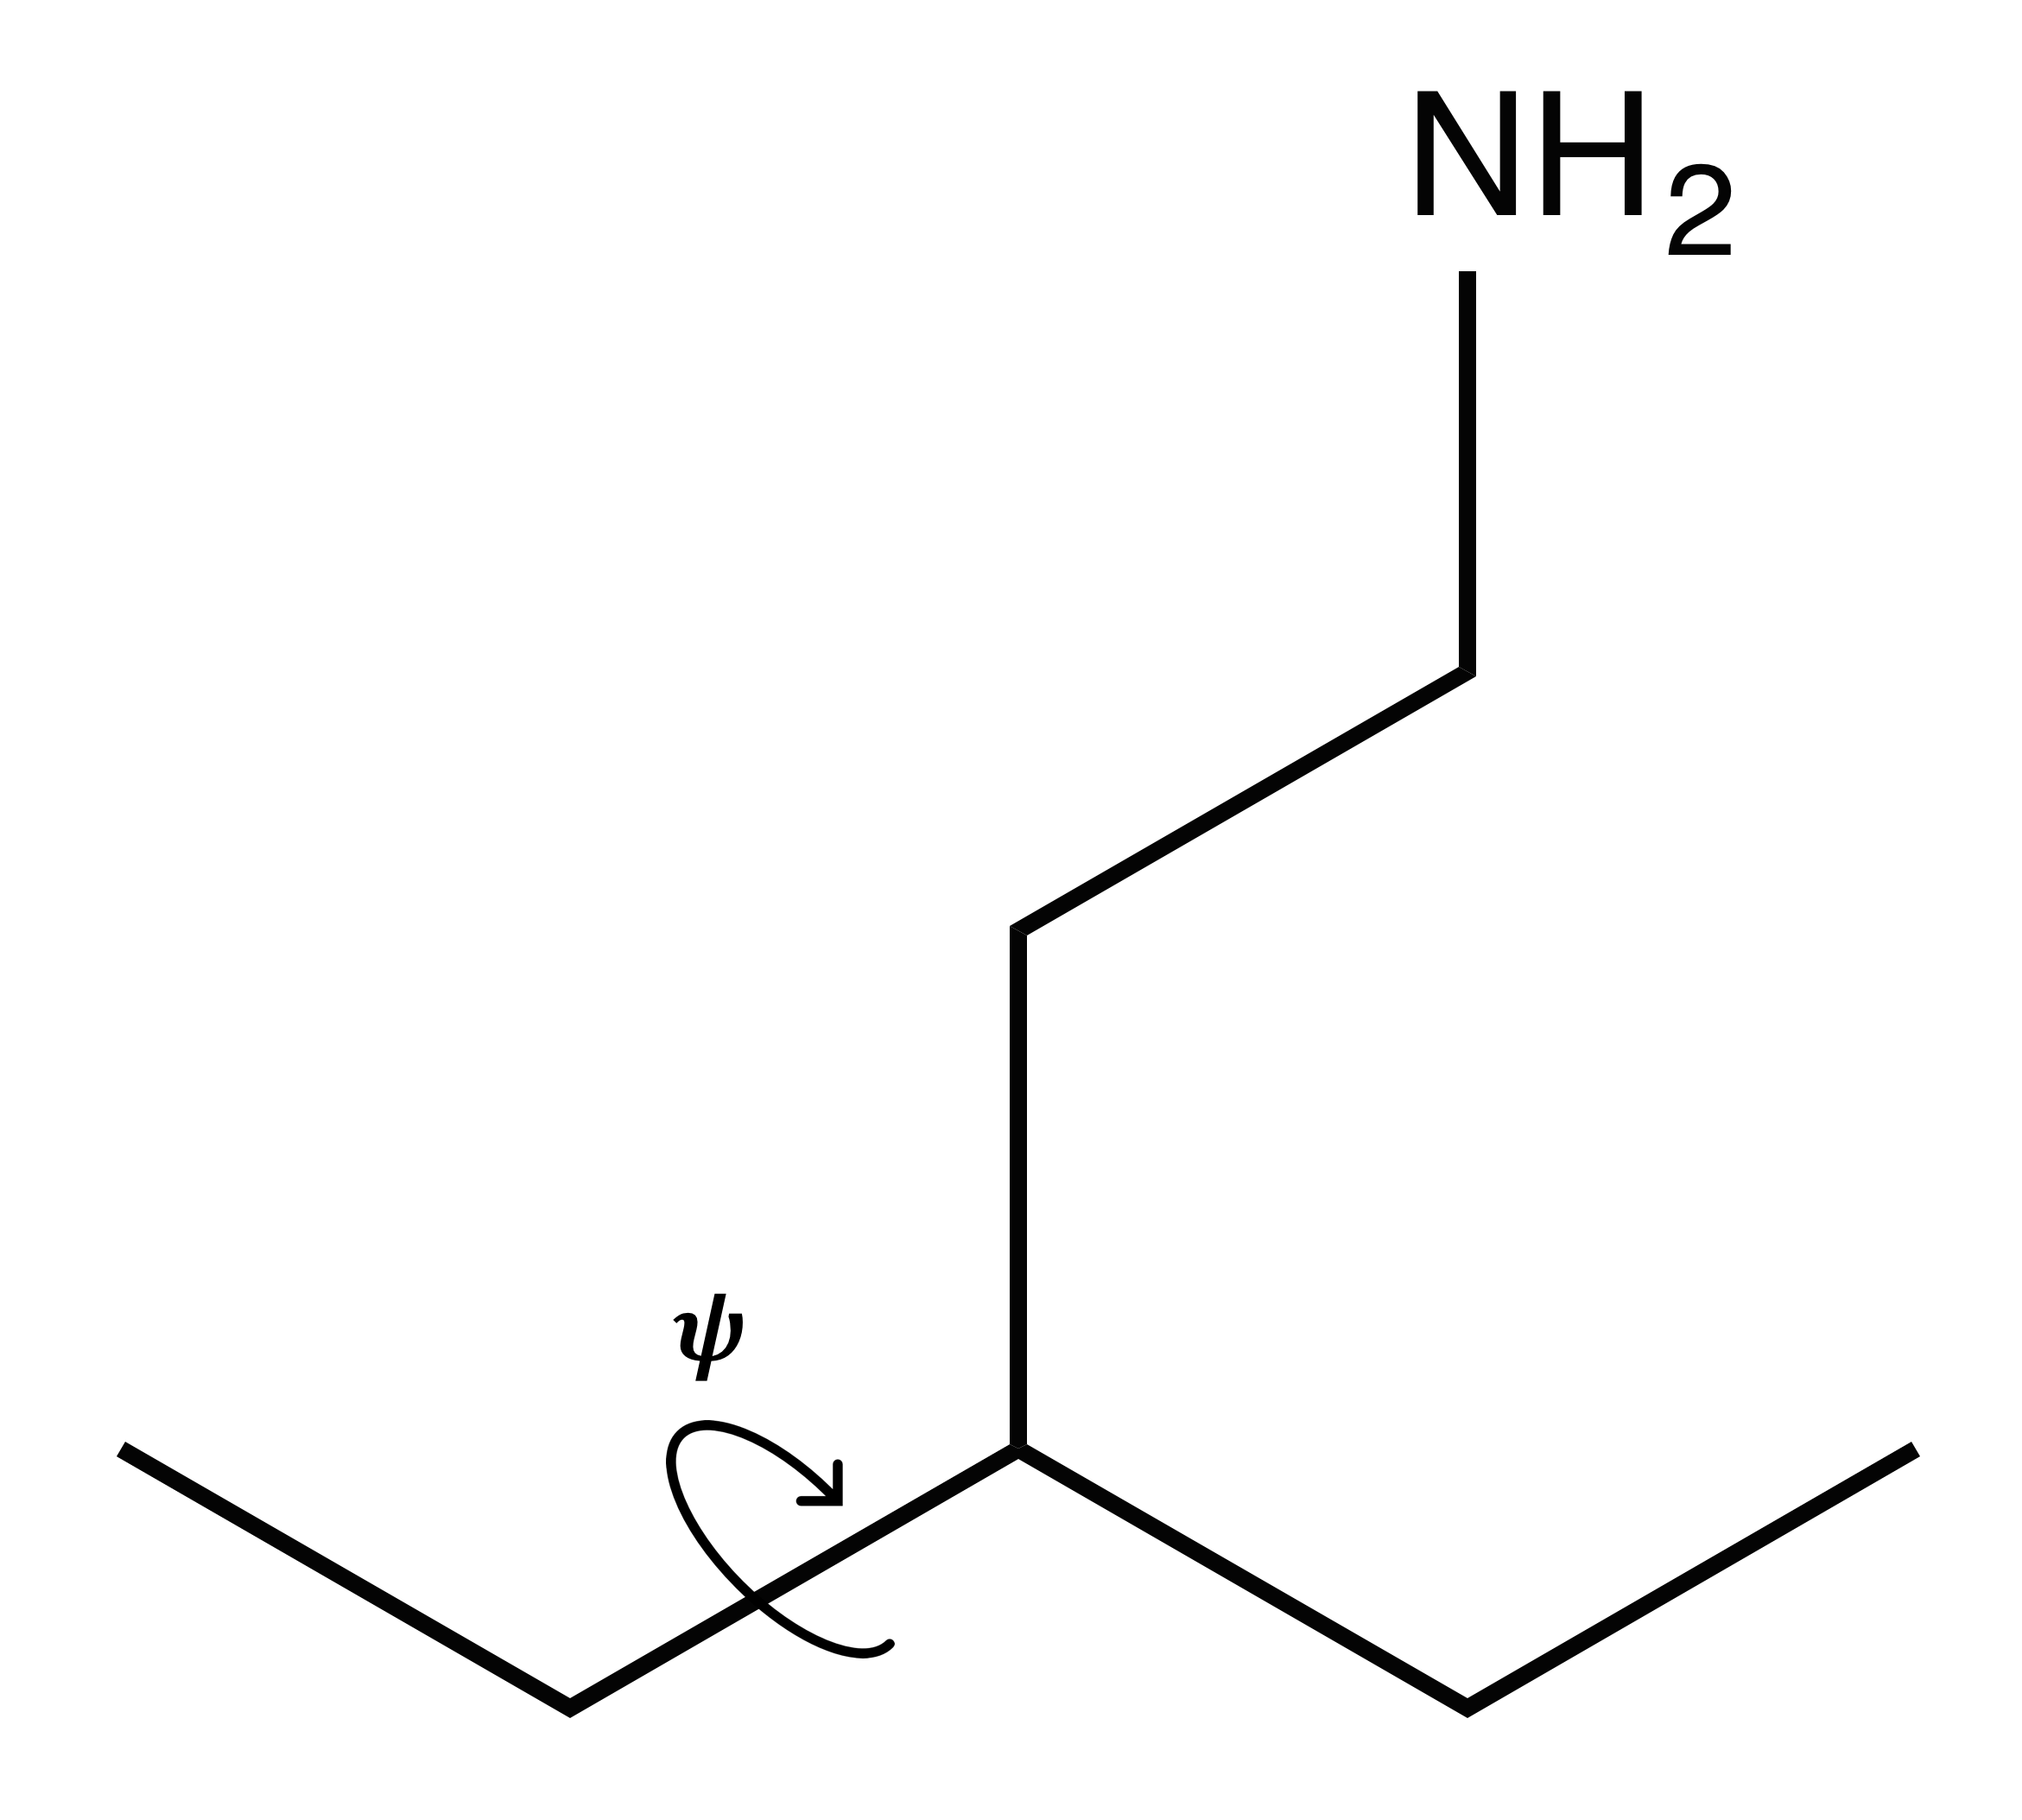
\includegraphics[scale=0.05]{Images/amino2} & 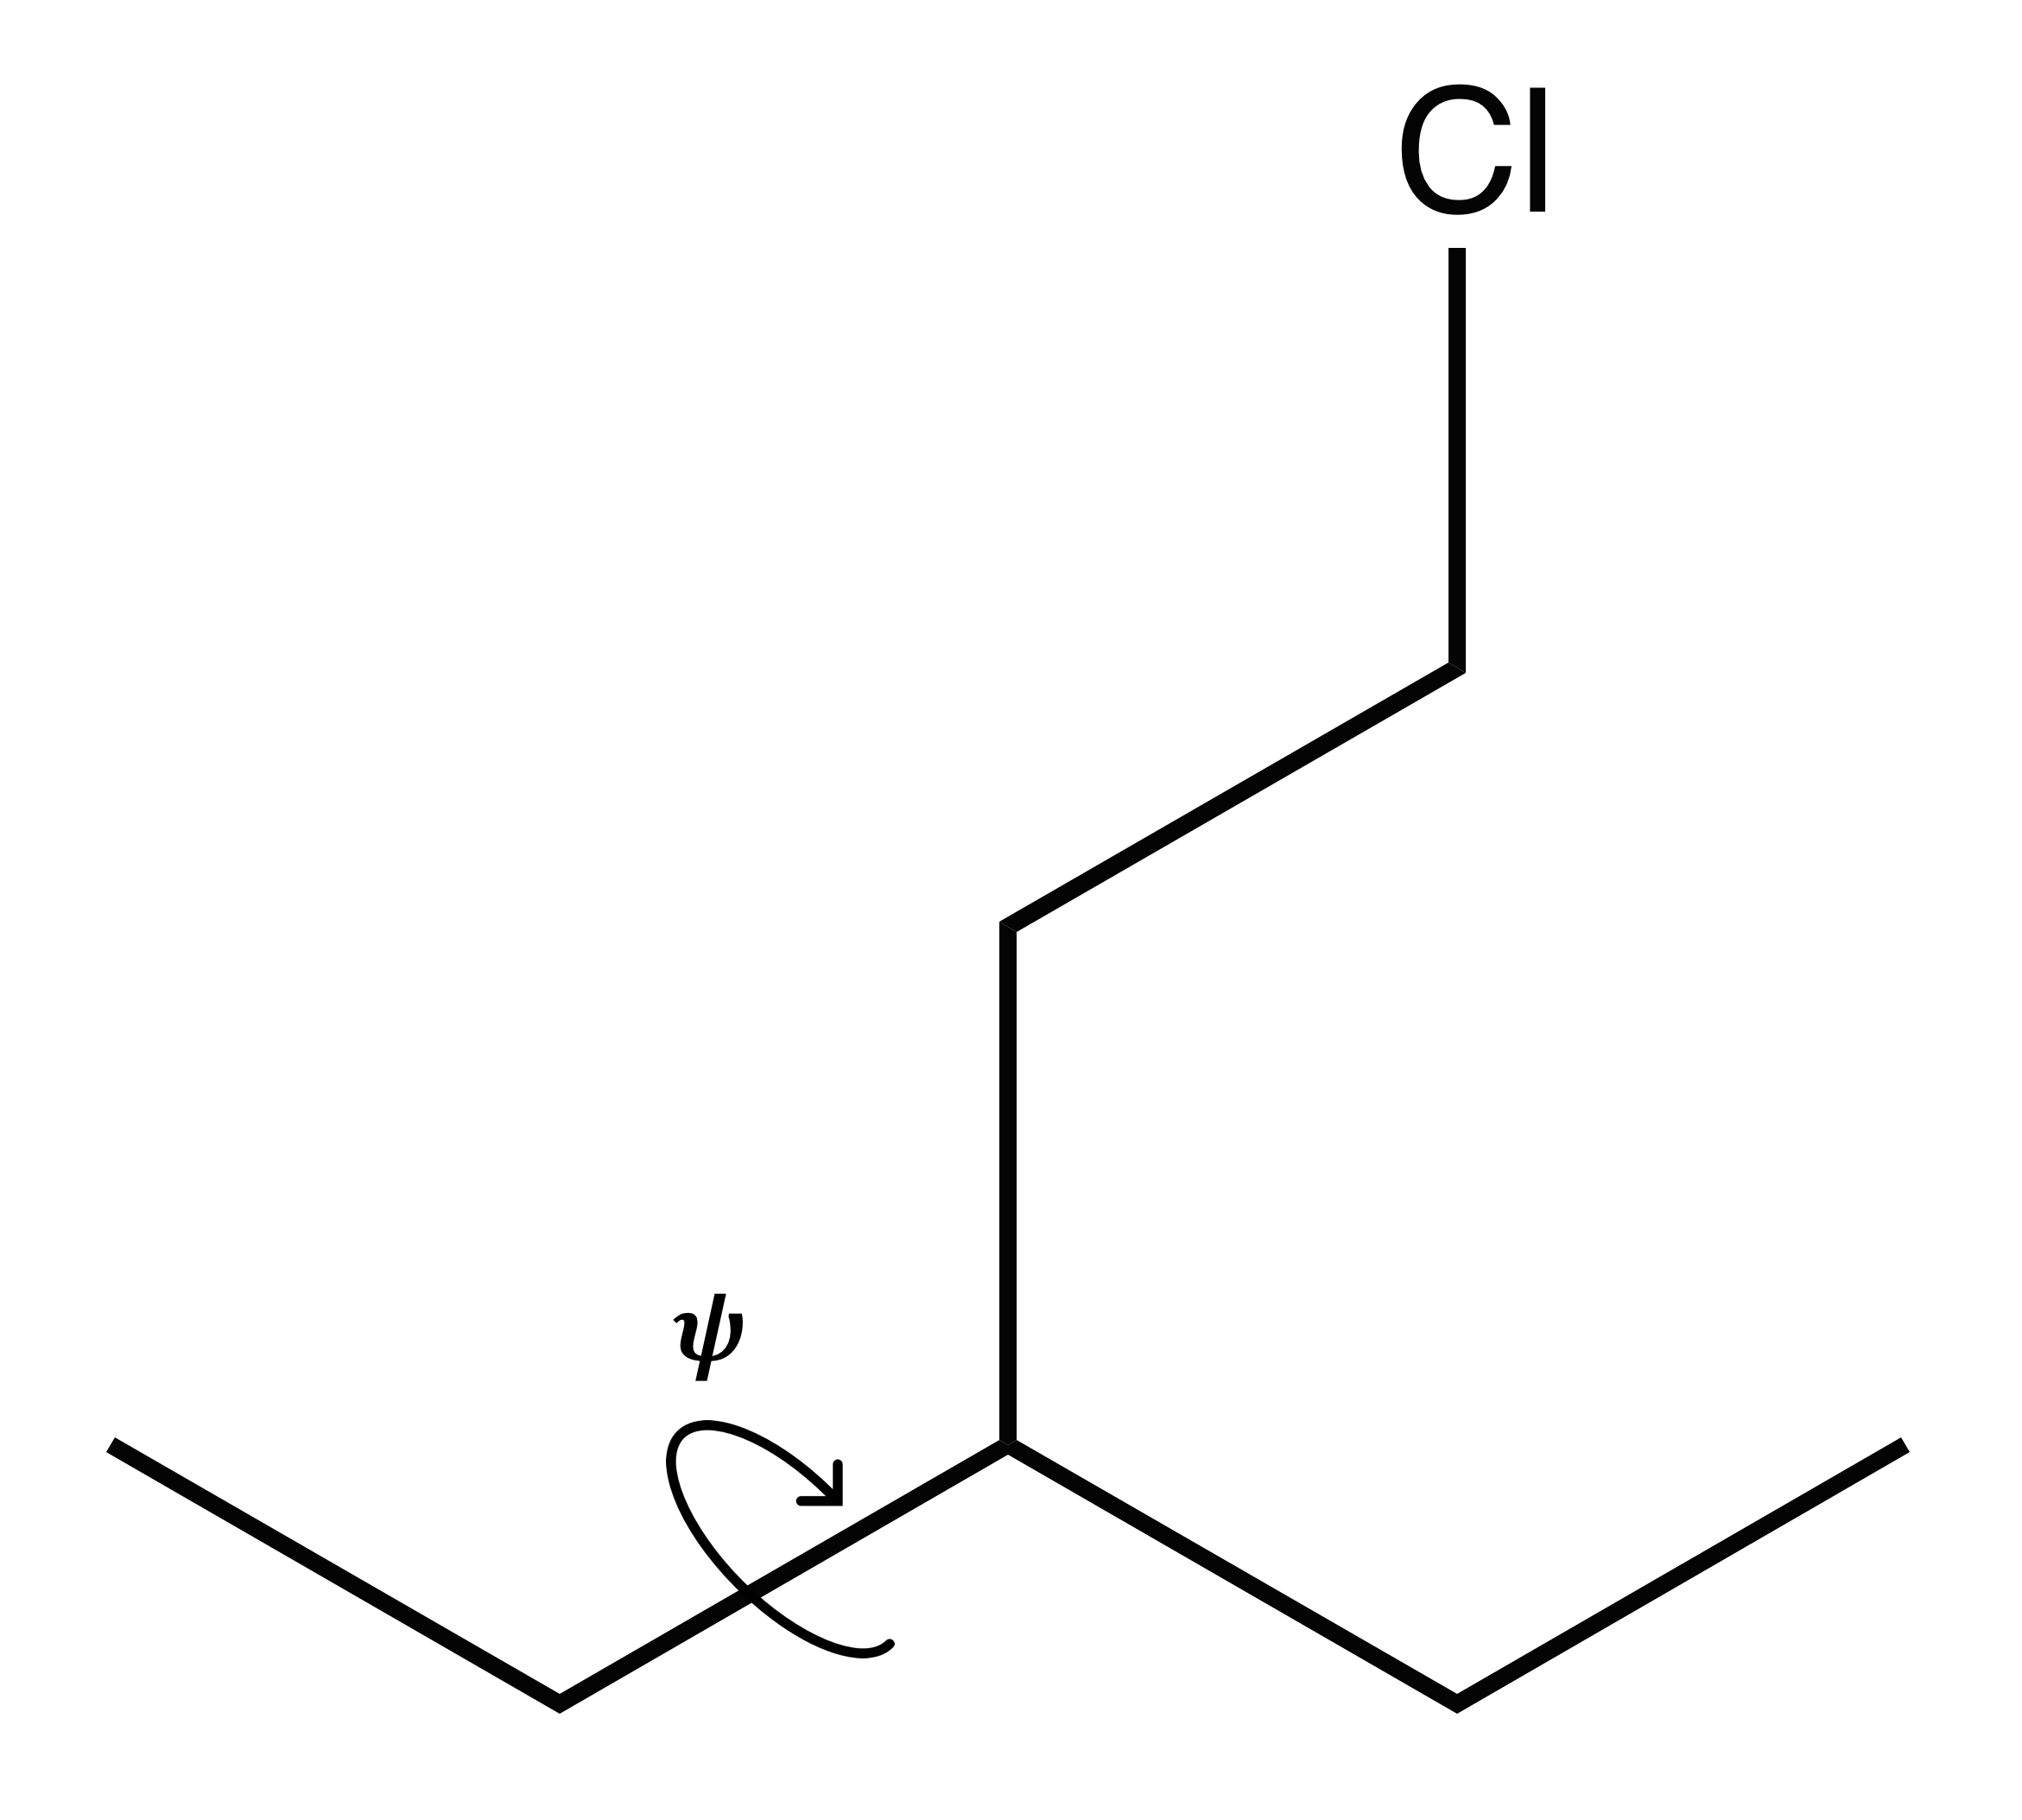
\includegraphics[scale=0.05]{Images/chloro2} & 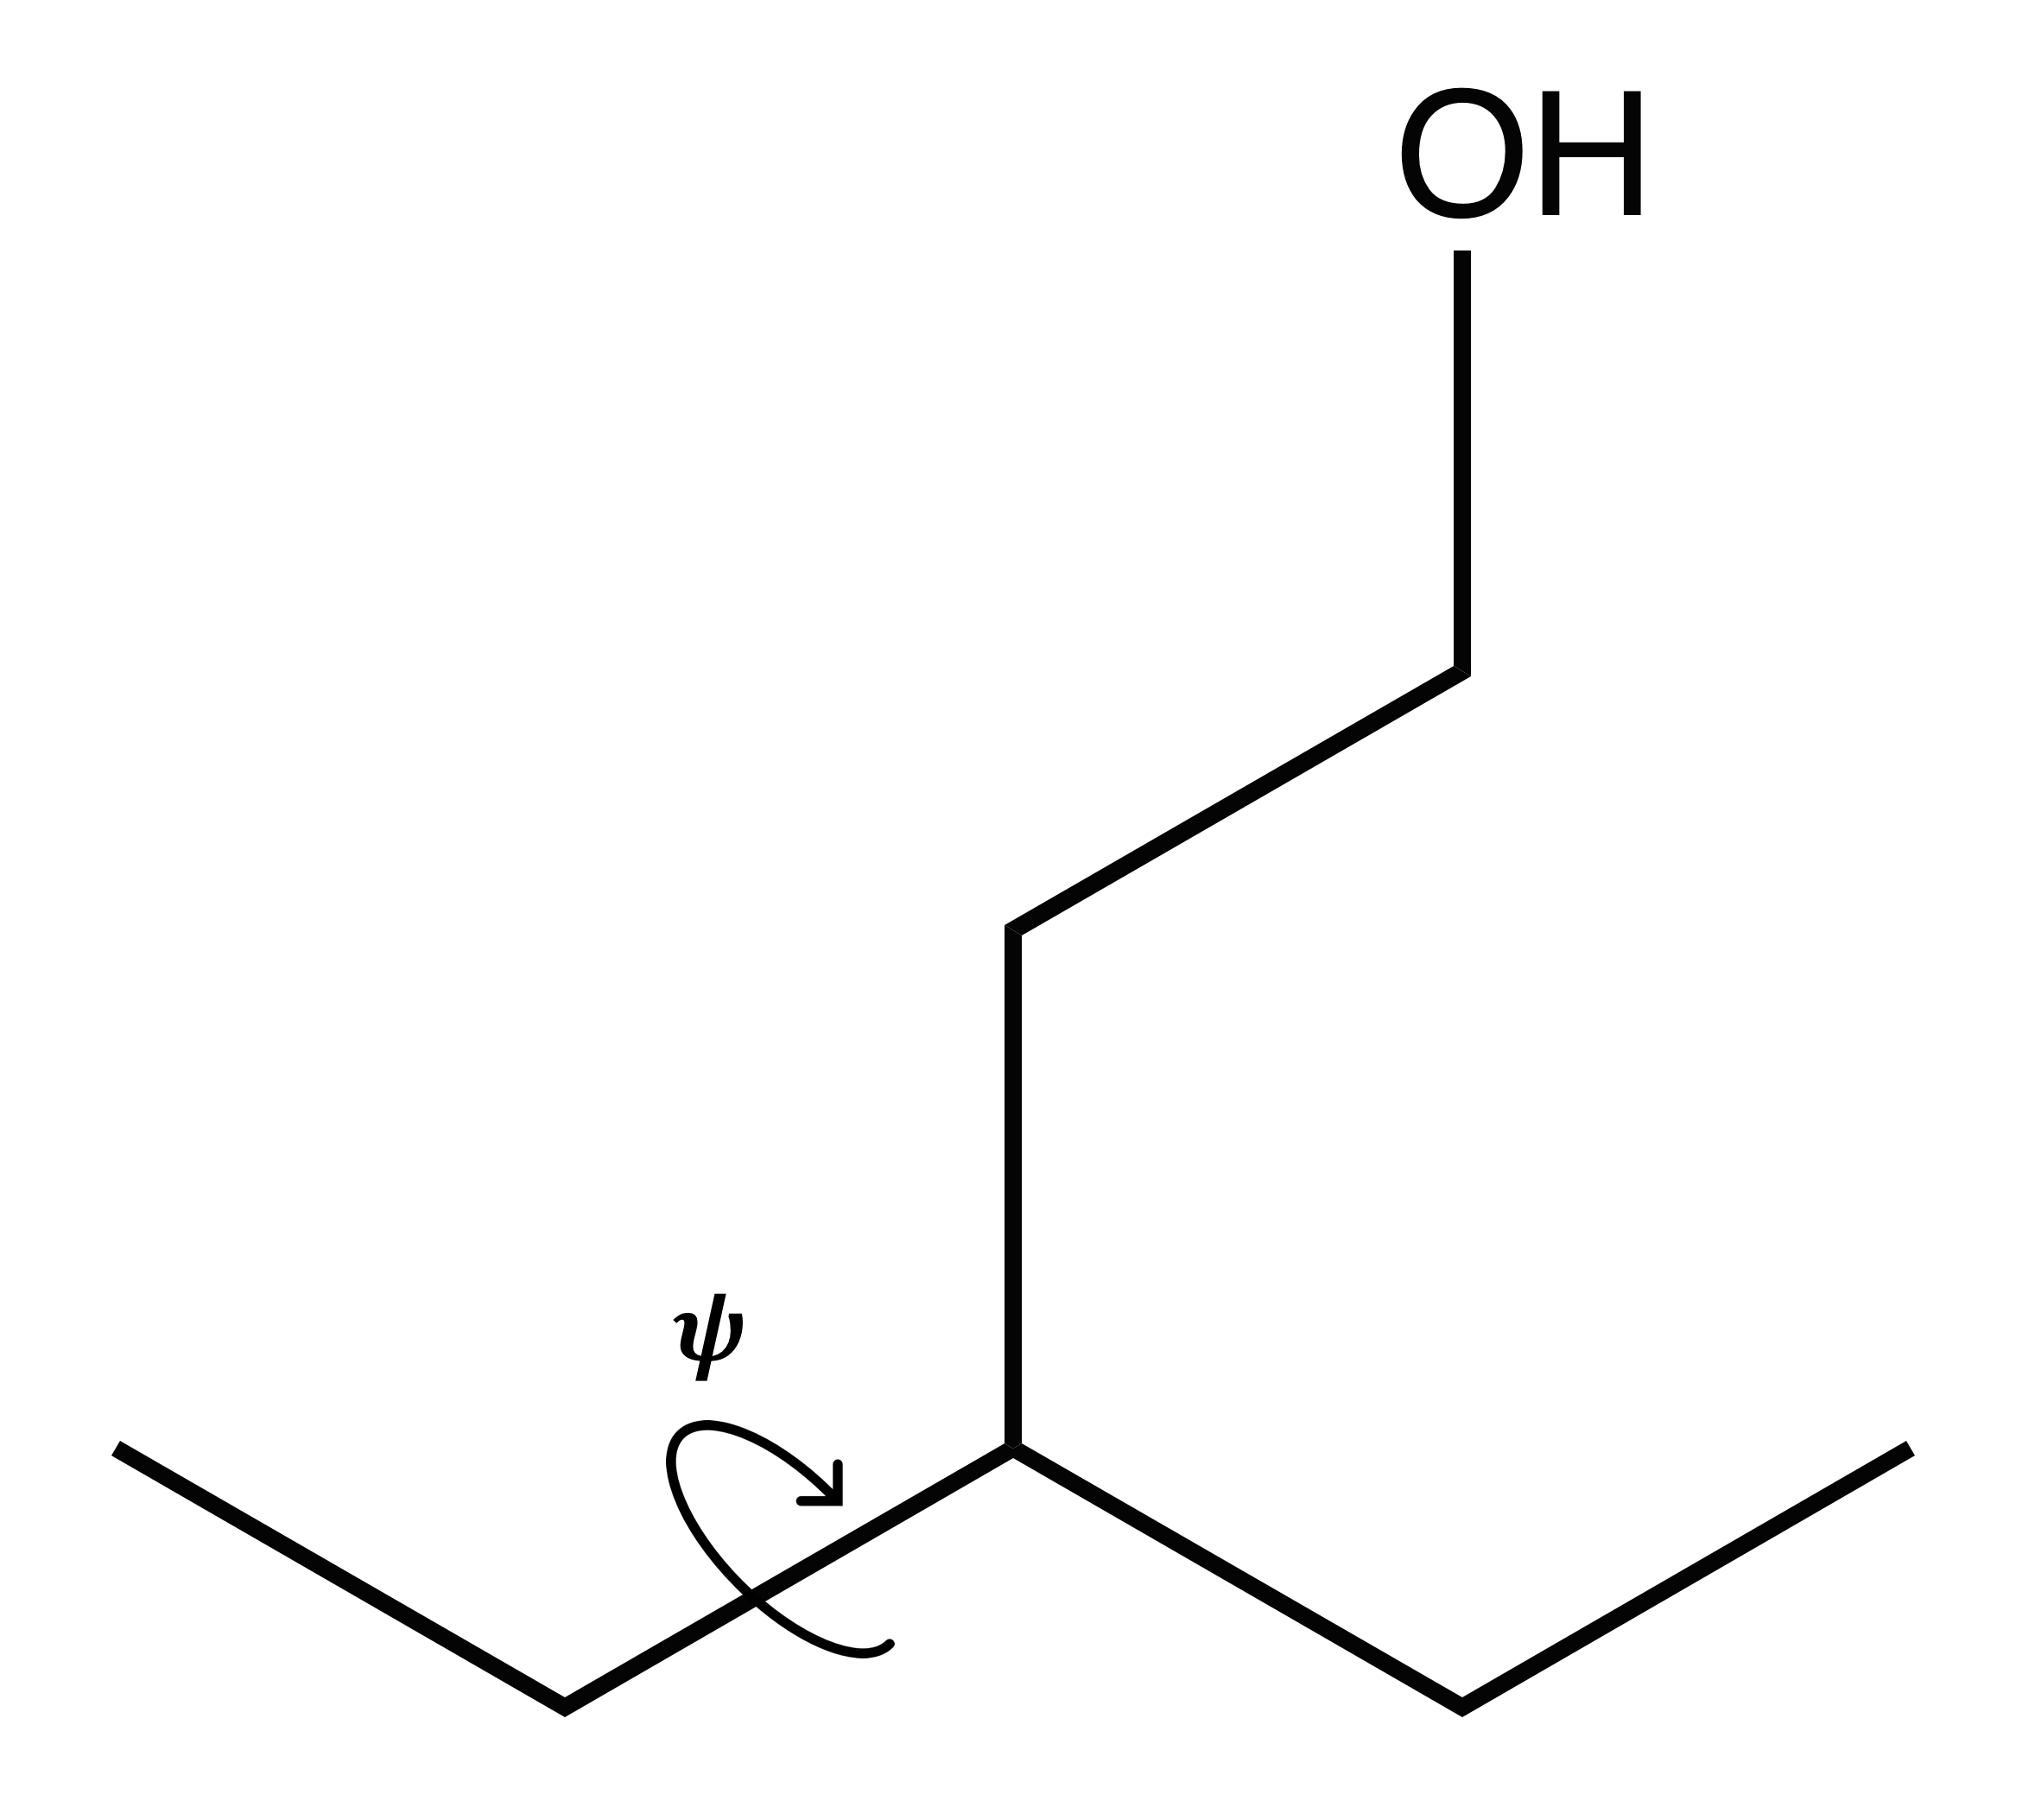
\includegraphics[scale=0.05]{Images/hydro2} & 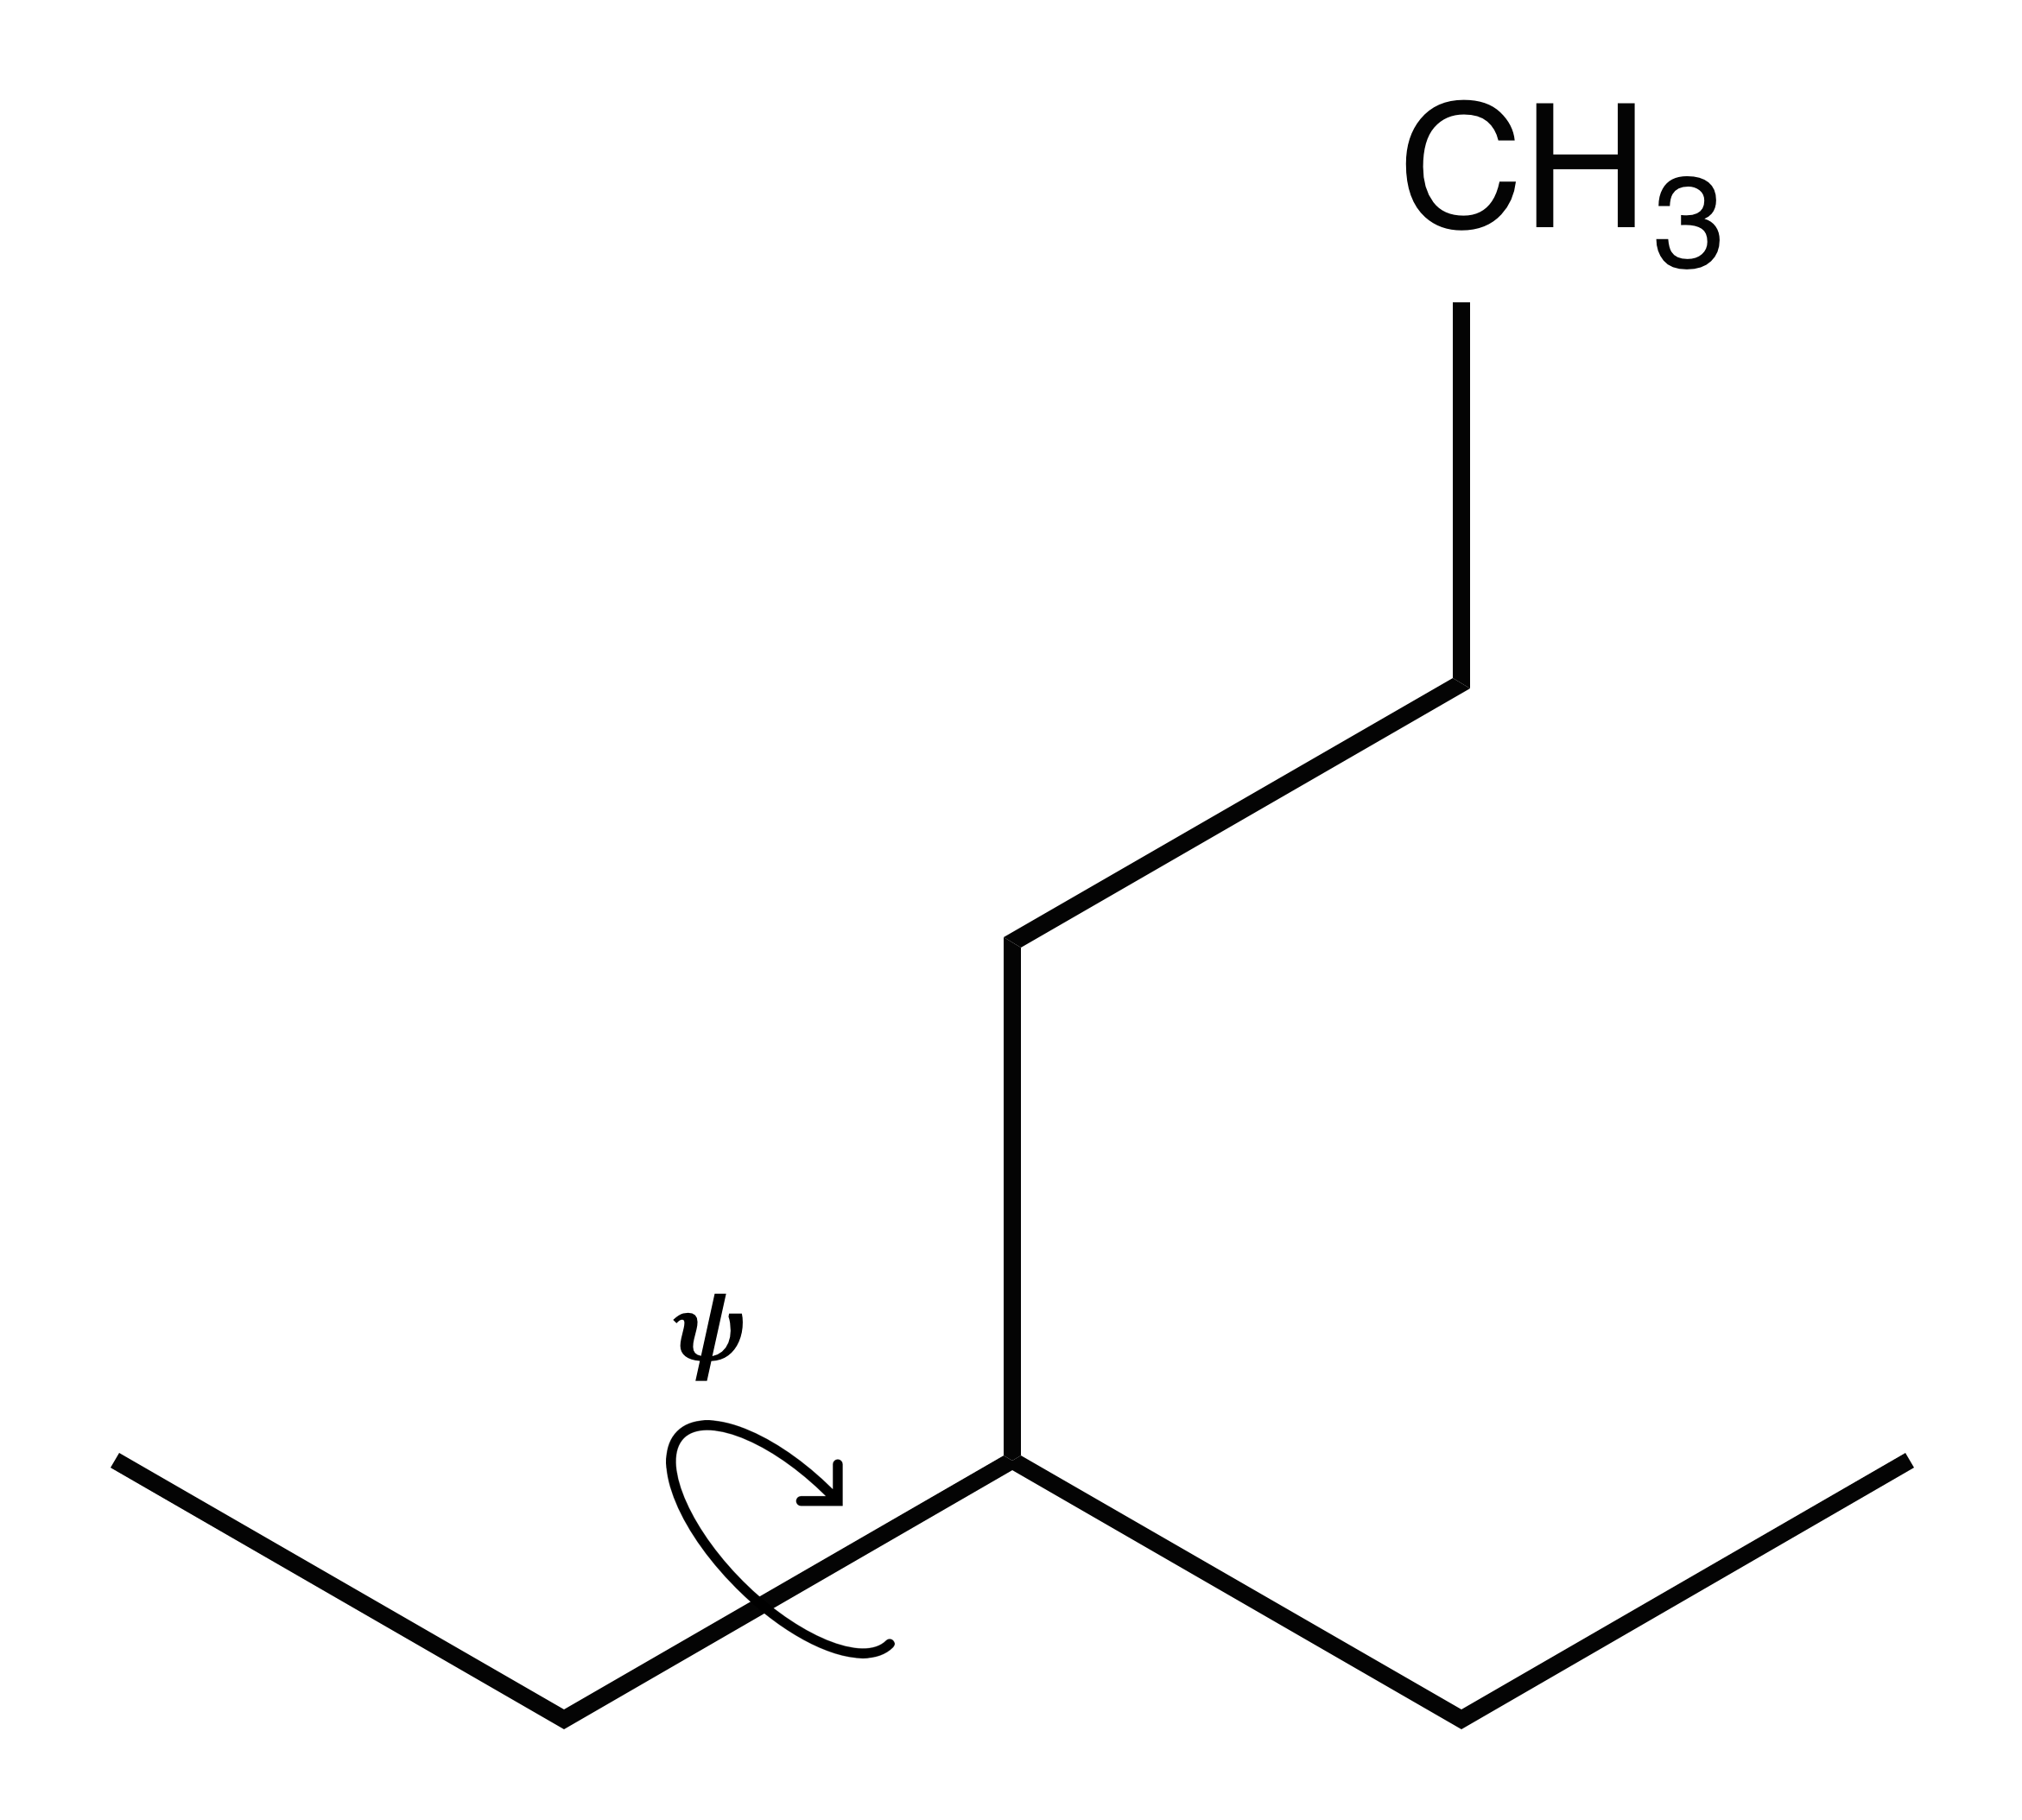
\includegraphics[scale=0.05]{Images/meth2} & 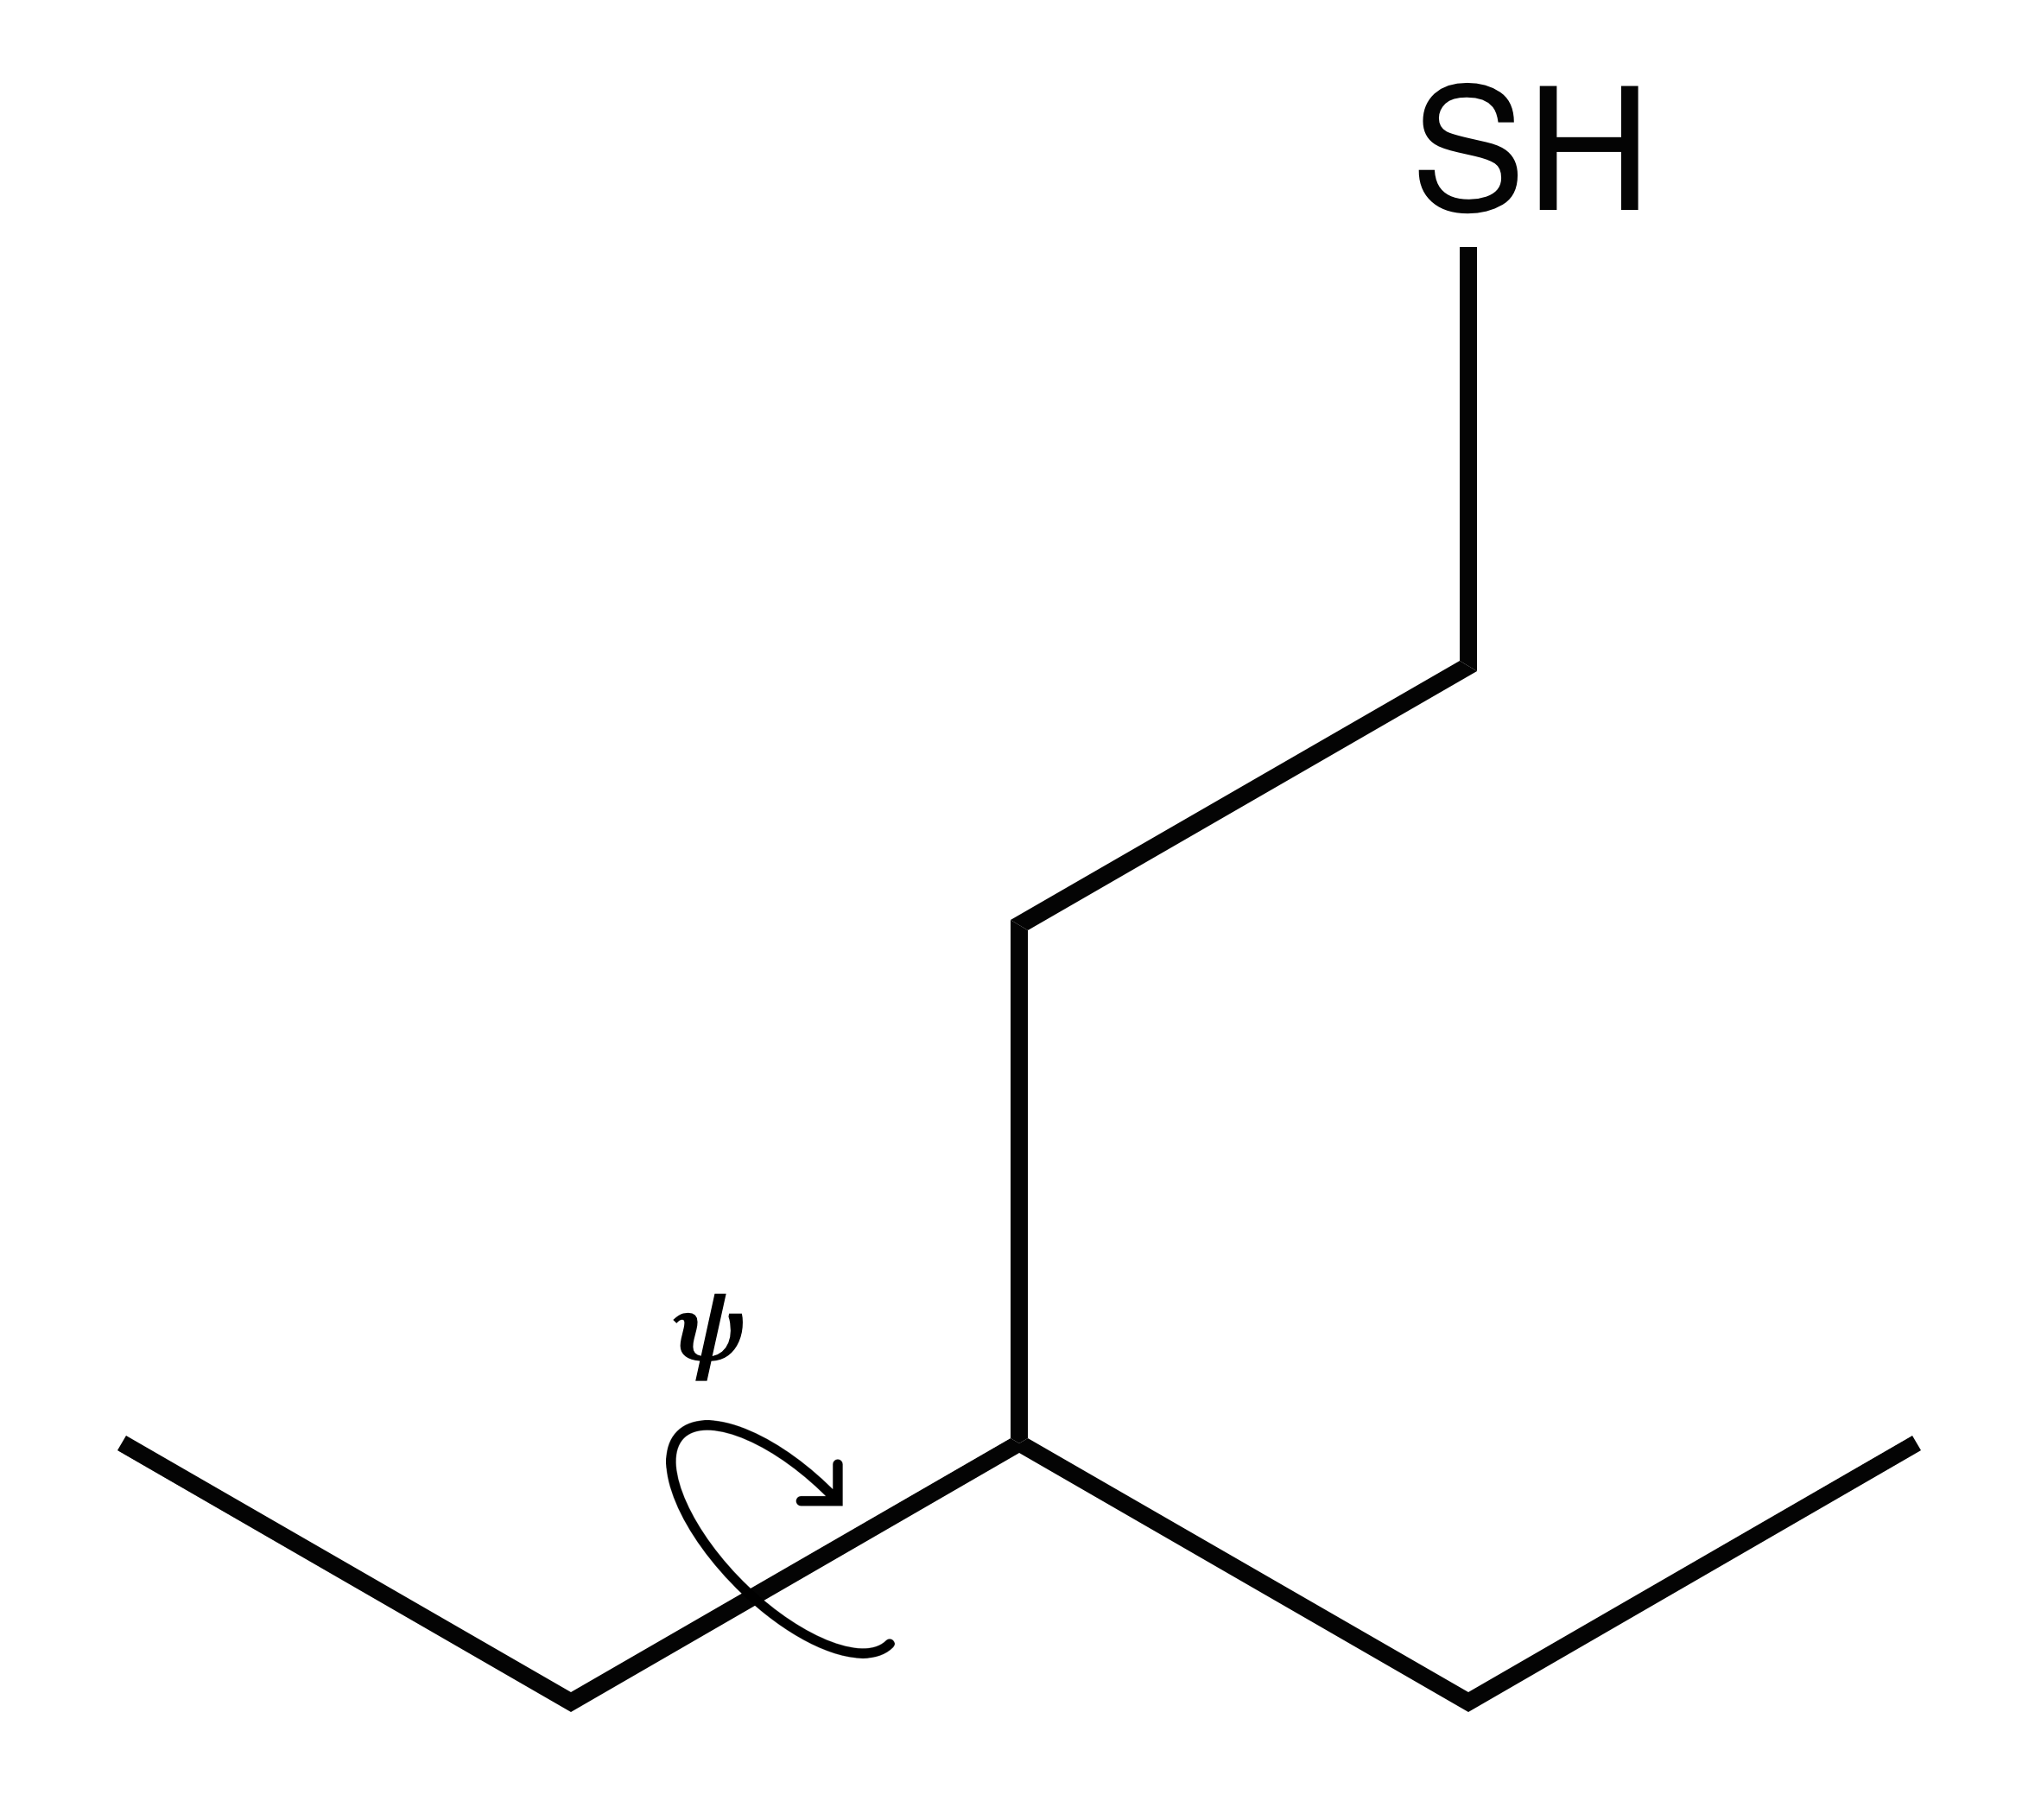
\includegraphics[scale=0.05]{Images/thio2} \\
 & 26642 & 26645 & 26647 & 26649 & 26652 \\ \hline
\end{tabular}
}
\caption{Chemical structures of the molecules for which torsional profiles were attained.}
\label{fig:structures}
\end{sidewaysfigure}

\section{Level of QM Theory}
All calculations were performed with the B3LYP density functional. First, the effect of basis set on the dihedral rotation profile was checked. Only the molecules shown in row 0 of figure~\ref{fig:structures} were used for this investigation. $\psi$ was fixed at 15$^{\circ}$ increments in the range [0,360$^{\circ}$], to give 24 regularly spaced conformations for each molecule. All calculations were performed at five different basis set levels (6-31G(d), 6-31+G(d), 6-311+G(2d,p), 6-311++G(2d,2p) and 6-311++G(3df,3p)) to determine the basis set error. RMSD results are given in Table~\ref{tb:basis_set_rmsd}.

\begin{table}[!tb]
\centering
\caption{RMSD values obtained from QM calculation of the dihedral rotational energy profile of the 0 row of molecules at different basis set levels. Two RMSD values are given. The first is the RMSD between the QM calculated energy values and the energy values determined from a two pass fitting of three dihedral terms to the energy profile (see Section~\ref{sec:FittingMethods}). The second is the RMSD between the energie values determined from fits at the given basis set level against the smallest basis set. All energies are in kJ~mol$^{-1}$.}
\label{tb:basis_set_rmsd}
\begin{tabular}{|c|l|c|c|}
\hline
Molecule                 & Basis Set        & RMSD w.r.t QM & RMSD w.r.t 6-31G(d) \\ \hline
\multirow{5}{*}{AMINO0}  & 6-31G(d)         & 2.07          & 0.00                \\ \cline{2-4} 
                         & 6-31+G(d)        & 2.59          & 0.43                \\ \cline{2-4} 
                         & 6-311+G(2d,p)    & 2.55          & 0.48                \\ \cline{2-4} 
                         & 6-311++G(2d,2p)  & 2.52          & 0.48                \\ \cline{2-4} 
                         & 6-311++G(3df,3p) & 2.51          & 0.37                \\ \hline
\multirow{5}{*}{CHLORO0} & 6-31G(d)         & 2.91          & 0.00                \\ \cline{2-4} 
                         & 6-31+G(d)        & 3.09          & 0.14                \\ \cline{2-4} 
                         & 6-311+G(2d,p)    & 3.13          & 0.63                \\ \cline{2-4} 
                         & 6-311++G(2d,2p)  & 3.13          & 0.70                \\ \cline{2-4} 
                         & 6-311++G(3df,3p) & 3.14          & 0.51                \\ \hline
\multirow{5}{*}{HYDRO0}  & 6-31G(d)         & 1.69          & 0.00                \\ \cline{2-4} 
                         & 6-31+G(d)        & 2.59          & 1.04                \\ \cline{2-4} 
                         & 6-311+G(2d,p)    & 2.48          & 1.10                \\ \cline{2-4} 
                         & 6-311++G(2d,2p)  & 2.45          & 1.13                \\ \cline{2-4} 
                         & 6-311++G(3df,3p) & 2.45          & 1.02                \\ \hline
\multirow{5}{*}{METH0}   & 6-31G(d)         & 3.26          & 0.00                \\ \cline{2-4} 
                         & 6-31+G(d)        & 3.44          & 0.21                \\ \cline{2-4} 
                         & 6-311+G(2d,p)    & 3.37          & 0.15                \\ \cline{2-4} 
                         & 6-311++G(2d,2p)  & 3.36          & 0.15                \\ \cline{2-4} 
                         & 6-311++G(3df,3p) & 3.39          & 0.15                \\ \hline
\multirow{5}{*}{THIO0}   & 6-31G(d)         & 3.36          & 0.00                \\ \cline{2-4} 
                         & 6-31+G(d)        & 3.56          & 0.18                \\ \cline{2-4} 
                         & 6-311+G(2d,p)    & 3.53          & 0.38                \\ \cline{2-4} 
                         & 6-311++G(2d,2p)  & 3.52          & 0.42                \\ \cline{2-4} 
                         & 6-311++G(3df,3p) & 3.56          & 0.37                \\ \hline
\end{tabular}
\end{table}  

\begin{figure}[htb]
\centering
\includegraphics[scale=0.7]{BasisSets/Figures/METH0/Combined}
\caption{Dihedral rotational energy profiles of METH0 $\psi$ calculated with 5 different basis sets.}
\label{fig:meth0_basis}
\end{figure}
    
\begin{figure}[htb]
\centering
\includegraphics[scale=0.7]{BasisSets/Figures/HYDRO0/Combined}
\caption{Dihedral rotational energy profiles of HYDRO0 $\psi$ calculated with 5 different basis sets.}
\label{fig:hydro0_basis}
\end{figure}

The results indicate that it should be acceptable for further calculations to be performed at the B3LYP/6-31G(d) level of theory. The two RMSD values report on different aspects of the calculations. The first (RMSD w.r.t QM) is the RMSD between the QM calculated energy values and the energy values calculated by performing a two-pass, linear least squares fitting to the QM energies, using the equation $U = \sum k_i \cdot \cos(m_i\theta + \delta)$ (see Section~\ref{sec:FittingMethods}). The least squares solves for $k_i$ and (indirectly) $\delta$. A negative $k_i$ gives $\delta = 180^{\circ}$, positive $\delta = 0^{\circ}$. The two-pass nature of the fit means that in the first pass, values of $m_i = 0 \to 6$ are used to generate linear equations, which are solved for $k_i$ and sorted based on the magnitude of $k_i$. The most important $N$ values of $m_i$ are then set as the only possible values, and passed through the same fitting process again. The RMSD between the QM energy values and the fitted energy values therefore gives an indication of how good the fit is. As shown in Table~\ref{tb:basis_set_rmsd}, the RMSD values between the QM calculated energy values and the fitted energy values are typically slightly higher than $k_bT$ (these RMSD values drop to less than 0.5 kJ mol$^{-1}$ when phase is also fitted), which shows that reasonable fits are obtained.\\
The second type of RMSD value reported in table~\ref{tb:basis_set_rmsd} are the RMSD values between the fitted energy values of the basis set of interest and the smallest basis set used here in (6-31G(d)). In all cases, these values remain below $\frac{1}{2}k_bT$, indicating that, in these molecules, there is not much gained from using a much larger basis set. This is further reinforced through inspection of the overlaid energy profiles for the cases exhibiting the least (Figure~\ref{fig:meth0_basis}) and most (Figure~\ref{fig:hydro0_basis}) deviation between the basis sets. Even the example with largest deviation between the dihedral rotational energy profiles, HYDRO0, the 6-31G(d) basis set still performs remarkably well when compared with the larger basis sets.\\
As such, all further QM calculations will be performed at the B3LYP/6-31G(d) level of theory.

\section{Fitting}
Torsional energy profiles can be described with a Fourier series, a potentially infinite set of cosines. MD simulations use a finite series of cosine terms, generally no more than three with multiplicities between 1 and 6, to represent this. Going from the raw data, comprising a set of energy values for each sampled torsion angle value, to the explicit series of cosines requires a fitting process. Given a raw data set spanning a full revolution of a torsional angle, there are a number of possible methods to fit a finite series of cosines to this data set, each of which involves performing a linear least squares (LLS) fit.

\subsection{Using simultaneous linear equations to fit to a Fourier series}

A Fourier series describing the torsional potential of conformation $j$ is given by
\begin{equation}
V_{j} = \sum_{i=1}^{N}k_{i}({1 + \cos(m_{i}\theta_{j} - \delta_{i})}),
\end{equation}
where $V_{j}$ is the dihedral potential energy of conformation $j$, $k_{i}$ is the amplitude of the $i$-th term, $m_{i}$ is the multiplicity associated with the $i$-th term, $\theta_{j}$ is the dihedral angle value of conformation $j$, and $\delta_{i}$ is the phase shift associated with the $i$-th term. In general usage, $\delta_{i}$ is limited to be either 0 or $\pi$, as other values give rise to an asymmetric potential. With this limit imposed, the Fourier series becomes:
\begin{equation}
V_{j} = C + \sum_{i=1}^{N}k_{i}\cos(m_{i}\theta_{j})\cos\delta_{i},
\end{equation}
where $C = \sum_{i=1}^{N}{k_{i}}$. As $\delta_{i}$ is limited to being either 0 or $\pi$, $\cos\delta_{i} = \pm 1$, meaning it can be ignored (a negative $k_{i}$ value can be converted to a positive value with a $\delta_{i}$ of $\pi$). By providing a list of $n$, $m_{i}$ values (multiplicity values comprise a limited number of integer values, and so do not need to be fit to), this becomes a series of $N$ simultaneous equations in $n$ variables, the $k_{i}$ values. This can then be written in the matrix form $b = Ax$:

\begin{equation} \label{eq:matrix}
\\
\begin{bmatrix}
V_{1} - c^{V}\\
V_{2} - c^{V}\\
\vdots\\
V_{N} - c^{V} 
\end{bmatrix}
 = 
\begin{bmatrix}
\cos(m_{1}\theta_{1})-c_{1}^A & \cos(m_{2}\theta_{1})-c_{2}^A & \ldots & \cos(m_{n}\theta_{1})-c_{n}^A \\
\cos(m_{1}\theta_{2})-c_{1}^A & \cos(m_{2}\theta_{2})-c_{2}^A & \ldots & \cos(m_{n}\theta_{2})-c_{n}^A \\
\vdots & \vdots & \ddots & \vdots \\
\cos(m_{1}\theta_{N})-c_{1}^A & \cos(m_{2}\theta_{N})-c_{2}^A & \ldots & \cos(m_{n}\theta_{N})-c_{n}^A \\
\end{bmatrix}
\begin{bmatrix}
k_{1} \\
k_{2} \\
\vdots \\
k_{n}
\end{bmatrix}
\end{equation}
where $c^V = \frac{1}{N}\sum_{j=1}^{N} V_{j}$ and $c_{i}^{A} = \frac{1}{N}\sum_{j=1}^{N} \cos(m_{i}\theta_{j})$. Solving this matrix using LLS gives the values of $k_{i}$. It is trivial to extended this method to fit to multiple torsional angles simultaneously (but note that this implies a different underlying philosophy of how best to parameterise torsional terms in a MM force field).

\subsubsection{Expanding to variable $\delta$}
As defined thus far, the matrix means of solving the simultaneous equations is not possible if $\delta_{i}$ is allowed to vary from 0/$\pi$. This is because the equations will become nonlinear, and so not solvable by LLS. However, there is a way to convert the nonlinear, variable phase (i.e. having to fit $k_{i}$ and $\delta_{i}$) equations into linear equations that can be dealt with by LLS.\\
If the individual torsional energy terms are treated as phasors, we can use the phasor addition rule to show that:
\begin{equation}
k_{i}(1 + \cos(m_{i}\theta - \delta_{i})) = k_{i,a}(1 + \cos(m_{i}\theta - \delta_{a})) + k_{i,b}(1 + \cos(m_{i}\theta - \delta_{b}))
\end{equation}
Then, if $\delta_{a}$ and $\delta_{b}$ are set to predetermined, non equal values, we are left with linear simultaneous equations which can be solved as per above. The solutions will give the values $k_{i,a}$ and $k_{i,b}$, but the desired results are $k_{i}$ and $\delta_{i}$. It is trivial to obtain these from the fitted values of $k_{i,a}$ and $k_{i,b}$:
\begin{eqnarray}
k_{i}^2  = & (k_{i,a}\cos\delta_{a} + k_{i,b}\cos\delta_{b})^2 + (k_{i,a}\sin\delta_{a} + k_{i,b}\sin\delta_{b})^2\\
\delta_{i} = & \arctan\Big(\frac{k_{i,a}\sin\delta_{a} + k_{i,b}\sin\delta_{b}}{k_{i,a}\cos\delta_{a} + k_{i,b}\cos\delta_{b}}\Big)
\end{eqnarray}

\subsection{Fitting methods}\label{sec:FittingMethods}

\begin{enumerate}[label=\alph*)]
\item \textbf{Single pass:} The set of linear equations (Eq.~\ref{eq:matrix}) is only generated and solved once. The raw data (torsional energy profile), a list of the multiplicity values to be included in the fit, and an optional limit, $N$ to the number of output multiplicities are provided. The matrices are generated and solved using all the provided multiplicity values, giving $k_{i}$ and $\delta_{i}$ values for each multiplicity $m_{i}$. The multiplicities are sorted in descending order based on the associated $k_{i}$ value. If a limit has been provided, the first $N$ multiplicity, amplitude and phase tuples are returned as the fitted results.
\item \textbf{Twin pass:} Two single pass fits are performed. The first pass is as described above, with a limit of $N$ tuples of multiplcity, amplitude and phase values returned. The second pass takes the returned $N$ multiplicities and performs a fit for only those multiplicity values. In this way, the refitted parameters will hopefully provide a better fit to the raw data than the `truncated' parameters, as they compensate slightly for the contribution of the discarded parameters.
\item \textbf{Multi pass:} Instead of relying on a sorted list of fit parameters to determine the $N$ parameter tuples to use, fits with all possible combinations of multiplicity values of length $N$ are performed. Thus, if the possible multiplicities are (1, 2, 3, 6), and $N = 3$, the fits performed will have multiplicities (1, 2, 3), (1, 2, 6), (1, 3, 6), and (2, 3, 6). Each fit performed has an error, $\epsilon$, associated with it, between the fit and the raw data. The fit with the lowest such error is determined to be the best fit, and the one to use. A simple error estimation function to use would be the RMSD:
\begin{equation}
\epsilon = \sqrt{\frac{1}{J}\sum_{j=1}^{J}\big(V_{\text{raw}}(\theta_{j}) - V_{\text{fit}}(\theta_{j})\big)^{2}}
\end{equation}
Of course, any other error estimation function is also usable.

\end{enumerate}

\subsection{Pruning outliers}
In some situations, it may be necessary to prune outliers from the data set. This is particularly the case with some of the MD torsional energy profiles, where the energy minimiser used to optimise the conformation for each value of $\psi$ is not as robust as the QM minimiser (I think). An example is shown in Figure~\ref{fig:outlier}. These outliers can have a significant effect on the fitted cosine terms, and so should be removed in a sensible manner. The current method is to iteratively fit cosine functions to the raw data, at each step removing the most deviant data point if the deviation from the fit is greater than some threshold (arbitrarily set to 1 kJ mol$^{-1}$). This method has flaws, particularly in that it is only really suited to handling isolated outliers. Small clusters of two or three outliers can, and do, cause issues in determing which data points to remove. A better method, involving robust regression, is under development.
\begin{figure}[htb]
\centering
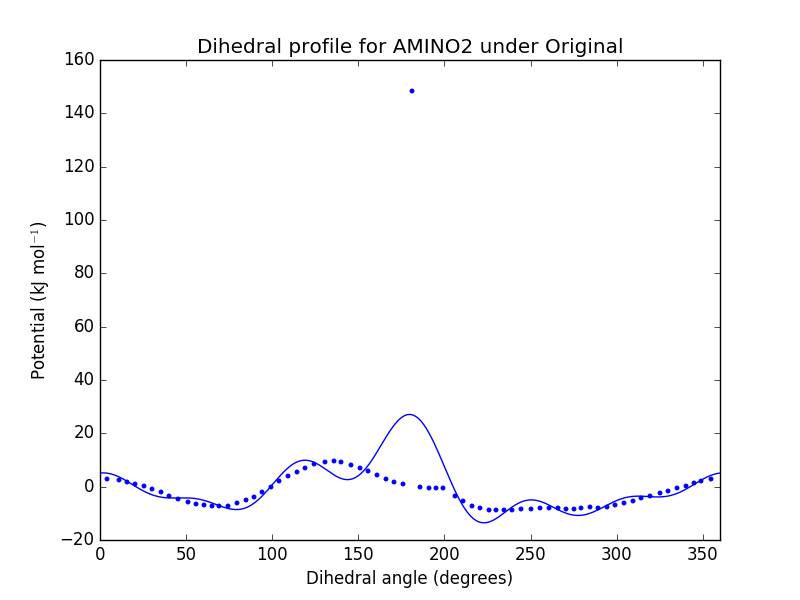
\includegraphics[scale=0.7]{Images/outlier}
\caption{Comparison of the MD dihedral rotational energy profile (points) and the fitted profile (line) for AMINO2. One datum is significantly removed from the general trend of the data and has a large effect on the fitted profile.}
\label{fig:outlier}
\end{figure}

\subsection{Comparing QM and MM data}
The torsional parameters should be fit to the difference between the dihedral rotational energy profiles obtained from QM calculations andfrom MD calculations using the MM force field but with the torsional term in question removed). There are several possible methods for obtaining this energy difference profile.
\begin{enumerate}
\item Difference between raw data sets. The MD energy value at each (fixed) $\psi$ value is subtracted from the QM energy value at that $\psi$ value. Though this approach is the most obvious means of determining the energy difference profile, it has a downside. Both the QM data (which is expensive to calculate) and the MD data (which has negligible computational cost) must be determined at the same $\psi$ values, which may not always be desirable or possible.
\item Difference between one raw data set and the fit to the other data set. In this approach, two fitting processes are performed. First, a series of cosine terms is fit to one set of raw data, for example a MD energy profile with high density sampling of $\psi$ values. The energy difference profile is computed between this fit and the other raw data set, and the second fit performed to this energy difference profile. This method does allow for differing sampling densities, which may be useful.
\item Difference between fits. As used in code of Purvi Gupta, a series of cosine terms is fit to each raw data set, the energy difference profile is computed as the difference between these two fits, and the final set of torsional parameters is fit to this energy difference profile. This is probably the most versatile fitting method. For example, a one pass fit, with no limit on $N$, is performed on the raw QM energy profile and the raw MD energy profile, utilising the ability to fit phase, and then a multi pass fit is performed on the energy difference profile, without fitting phase. In this way, very good fits to the QM and MD data could be obtained, while allowing the energy difference profile to be fit in a manner consistent with the force field parameterisation philosophy.
\end{enumerate}

\section{Results}
\subsection{Fitting methods}
Each of the three fitting methods described was tested on 50,000 sets of randomly generated periodic torsional energy profiles, and 113 sets of real torsional energy profiles from QM, all-atom MD (AA-MD) and united atom MD (UA-MD). The `random' energy profiles were generated from Fourier series of all multiplicities up to 12. Each term had a randomly generated amplitude and phase as well as a small amount of noise applied. Noise was applied by multiplying the energy calculated at each dihedral angle by a random, uniformly distributed value between 0.9 and 1.1. Fitting was performed with $N = 3$ to match with the general limit on number of torsional terms.\\
Though the data is not shown (it's an 80MB plain text file), fitting to the random torsional energy profiles gave identical results within all phased fits and within all non-phased fits. Non-phased fits naturally had a larger RMSD when compared with the phased fit, but all three non-phased fit results were the same in terms of fitted amplitude and phase (and thus RMSD values were identical), as were all three phased fit results.
Fitting to the `real' data gave similar results. The two pass and multi pass fitting methods gave identical results ($k_i$ and $\delta_i$ were identical), as would be expected (given the same number of torsional values to fit, two-pass and multi-pass fitting methods would be expected to give the same results as the second pass of the two-pass method would be fitting to the same set of possible cosine multiplicities as the `best' multi-pass step would be). One pass fitting had RMSD values slightly larger than the two/multi pass methods; on average a 0.001\% increase (from the RMSD of the two/multi pass methods) for the non-phased fit, and a 0.05\% increase for the phased fits.
The difference between the results of fitting to `random' versus `real' torsional energy profiles (i.e. the fact that the fits to the `real' data showed slight differences in the goodness of fit between the one pass and the other fitting methods, whereas the fits to the `random' data did not) probably arises from the way noise was added to the `random' data. In the `real' data, there is a small amount of noise (defining noise as when the calculated energy value does not exactly match the fitted energy value) in each energy value. However, a few data points have much larger deviation from the fitted periodic function. Such large deviations were not included in the `random' data, as small amounts of noise were applied to the all the generated data points, not large amounts to a few. Regardless, these results indicate that it should be perfectly reasonable to perform fitting with the cheapest single pass method, without noticeably affecting the quality of the fits.

\subsection{Comparing QM and MM data}
The three methods for comparing the QM and MM data to determine the energy difference profile to fit to were compared. These tests were run on the -1 series of molecules. The tests were:
\begin{itemize}
\item $\Delta_{\text{EP}} = \text{QM}_{\text{raw}} - \text{MD}_{\text{raw}}$. Phased and non-phased fits to $\Delta_{\text{EP}}$; MD torsional energy profiles computed using both AA and UA (4 cases).
\item $\Delta_{\text{EP}} = \text{QM}_{\text{raw}} - \text{MD}_{\text{fit}}$, where $\text{MD}_{\text{fit}}$ is the phased or non-phased fit to $\text{MD}_{\text{raw}}$. Phased and non-phased fits to $\Delta_{\text{EP}}$; MD torsional energy profiles computed using both AA and UA (8 cases).
\item $\Delta_{\text{EP}} = \text{QM}_{\text{fit}} - \text{MD}_{\text{raw}}$, where $\text{QM}_{\text{fit}}$ is the phased or non-phased fit to $\text{QM}_{\text{raw}}$. Phased and non-phased fits to $\Delta_{\text{EP}}$; MD torsional energy profiles computed using both AA and UA (8 cases).
\item $\Delta_{\text{EP}} = \text{QM}_{\text{fit}} - \text{MD}_{\text{fit}}$, where $\text{QM}_{\text{fit}}$ and $\text{MD}_{\text{fit}}$ are the phased or non-phased fits to $\text{QM}_{\text{raw}}$ and $\text{MD}_{\text{raw}}$, respectively (either phased or non-phased fitting for both, i.e. \emph{not} mixing the fit type). Phased and non-phased fits to $\Delta_{\text{EP}}$ (non-phased can be fit to phased $\Delta_{\text{EP}}$, but phased cannot be fit to non-phased $\Delta_{\text{EP}}$); MD torsional energy profiles computed using both AA and UA (6 cases).
\end{itemize}
These give a total of 26 different tests that were performed on the 5 molecules in the -1 series. Fits to raw torsional energy profiles were performed with single pass fitting with unlimited $N$. Fits to $\Delta_{\text{EP}}$ were performed with single pass fitting and $N = 3$. As the aim is to calculate the parameters of the MM torsional term such that the raw MD torsional energy profile plus the fitted torsional term equals the raw QM torsional energy profile, the RMSD of a particular fit is the RMSD of the raw MD energy profile plus the fitted energy profile from the the raw QM energy profile. Results are presented in Table~\ref{tb:differencedata}. As expected, fitting phase in addition to fitting amplitude provides much lower RMSD values. The one exception to this is when one of the raw energy profiles is fit without phase, and $\Delta_{\text{EP}}$ is fit with phase. This indicates that a higher level fit should not be performed to a profile obtained using a lower level fit. Otherwise, all fitting methods perform similarly across all phased or unphased cases, indicating that the use of phasing has the largest impact on how well the fitted torsional term reproduces $\Delta_{\text{EP}}$. Given that obtaining phase for the torsional terms is not generally necessary, and in order to have the best flexibility and extensibility, all further fits of torsional parameters will use a phased fit to the raw torsional energy profiles, followed by a non-phased fit to $\Delta_{\text{EP}}$. This allows for a phased fit to the $\Delta_{\text{EP}}$ energies if required.

\begin{table}[!tb]
\centering
\caption{RMSD values between raw QM torisional energy profile and the raw MD torsional energy profile plus the fitted torsional term.}
\label{tb:differencedata}
\resizebox{\textwidth}{!}{%
\begin{tabular}{|c|c|c|c|c|c|c|c|}
\hline
Type                 & QM                     & MD                     & Phase & AMINO-1 & CHLORO-1 & HYDRO-1 & THIO-1 \\ \hline
\multirow{13}{*}{AA} & \multirow{6}{*}{raw}   & \multirow{2}{*}{raw}   & No    & 2.1543  & 1.3550   & 1.2465  & 1.0747 \\ \cline{4-8} 
                     &                        &                        & Yes   & 0.6931  & 0.7976   & 0.7402  & 0.3368 \\ \cline{3-8} 
                     &                        & \multirow{2}{*}{fit}   & No    & 2.1583  & 1.3556   & 1.2471  & 1.0744 \\ \cline{4-8} 
                     &                        &                        & Yes   & 2.1766  & 3.0890   & 3.0203  & 2.9784 \\ \cline{3-8} 
                     &                        & \multirow{2}{*}{phase} & No    & 2.1583  & 1.3552   & 1.2467  & 1.0755 \\ \cline{4-8} 
                     &                        &                        & Yes   & 0.6952  & 0.7988   & 0.7418  & 0.3385 \\ \cline{2-8} 
                     & \multirow{3}{*}{fit}   & \multirow{2}{*}{raw}   & No    & 2.1583  & 1.3556   & 1.2471  & 1.0744 \\ \cline{4-8} 
                     &                        &                        & Yes   & 3.9048  & 3.8936   & 3.7885  & 3.7613 \\ \cline{3-8} 
                     &                        & fit                    & No    & 2.1583  & 1.3556   & 1.2471  & 1.0744 \\ \cline{2-8} 
                     & \multirow{4}{*}{phase} & \multirow{2}{*}{raw}   & No    & 2.1585  & 1.3552   & 1.2468  & 1.0759 \\ \cline{4-8} 
                     &                        &                        & Yes   & 0.6952  & 0.7988   & 0.7418  & 0.3385 \\ \cline{3-8} 
                     &                        & \multirow{2}{*}{phase} & No    & 2.1583  & 1.3552   & 1.2466  & 1.0755 \\ \cline{4-8} 
                     &                        &                        & Yes   & 0.6952  & 0.7988   & 0.7418  & 0.3385 \\ \hline   
\multirow{13}{*}{UA} & \multirow{6}{*}{raw}   & \multirow{2}{*}{raw}   & No    & 1.2136  & 1.0947   & 1.1666  & 1.1781 \\ \cline{4-8} 
                     &                        &                        & Yes   & 0.4858  & 0.4553   & 0.5128  & 0.4325 \\ \cline{3-8} 
                     &                        & \multirow{2}{*}{fit}   & No    & 1.2145  & 1.0958   & 1.1777  & 1.1793 \\ \cline{4-8} 
                     &                        &                        & Yes   & 3.9231  & 4.0898   & 3.9322  & 4.0949 \\ \cline{3-8} 
                     &                        & \multirow{2}{*}{phase} & No    & 1.2138  & 1.0948   & 1.1666  & 1.1783 \\ \cline{4-8} 
                     &                        &                        & Yes   & 0.4890  & 0.4576   & 0.5153  & 0.4374 \\ \cline{2-8} 
                     & \multirow{3}{*}{fit}   & \multirow{2}{*}{raw}   & No    & 1.2145  & 1.0958   & 1.1777  & 1.1793 \\ \cline{4-8} 
                     &                        &                        & Yes   & 3.8920  & 3.8540   & 3.7845  & 3.7986 \\ \cline{3-8} 
                     &                        & fit                    & No    & 1.2145  & 1.0958   & 1.1777  & 1.1793 \\ \cline{2-8} 
                     & \multirow{4}{*}{phase} & \multirow{2}{*}{raw}   & No    & 1.2138  & 1.0948   & 1.1667  & 1.1783 \\ \cline{4-8} 
                     &                        &                        & Yes   & 0.4890  & 0.4576   & 0.5153  & 0.4374 \\ \cline{3-8} 
                     &                        & \multirow{2}{*}{phase} & No    & 1.2138  & 1.0948   & 1.1673  & 1.1783 \\ \cline{4-8} 
                     &                        &                        & Yes   & 0.4890  & 0.4576   & 0.5153  & 0.4374 \\ \hline
\end{tabular}
}
\end{table}

%\subsection{Further geometry restraints}
%It was noticed that the torsional energy profiles of the series 1 and 2 molecules had some strange fluctuations in it that could not be chemically explained. Upon investigation of these fluctuations, it was found to be caused by unwanted rotation about the symmetric dihedral of the dihedral of interest. It is likely that these fluctuations affect the outcome of the fitting procedure to some extent. Thus, it would be nice to remove these fluctuations somehow. The obvious way to do this is by adding extra restraints to the QM calculations forcing the

\subsection{Functional group shifting}
The effect on the torsional energy profile as functional groups move further from the dihedral of interest is important to investigate, as it affects the generalisabilitly and transferability of force field torsional terms. As a function group moves further from the dihedral of interest, its effect on the torsional energy profile should be diminished, until such a point is reached where there is effectively no influence. The 0 to 2 series of molecules (Figure~\ref{fig:structures}) aims to investigate this effect. Each molecule has the functional group moved one carbon further from the dihedral of interest than the previous molecule in the series. In all cases, the dihedral of interest is the same, a carbon-carbon single bond between two $sp^3$ hybridised carbons. As such, the fitted terms are dominated by a term with multiplicity of 3. Comparing parameters of the fitted torsional terms across all the molecules will give an indication of how much effect the functional group is having on the given torsional angle. These values are given in Table~\ref{tb:functionshift}.\\
It is clear to see that the AA and UA fits give differing results. Given that GROMOS is a UA forcefield, it seems best to determine generalisations based on the UA results and apply these to the AA systems, even if the AA systems do not exactly follow the same trends. With that in mind, in the 2 series of molecules, the effect of the functional group looks to be negligible. The standard deviation of the values of the amplitude across the series is much lower than is the case with the 0 and 1 series. This is also the case for the AA results, although to a lesser degree. It appears, therefore, that torsional energy profiles could be calculated from small reference molecules where only heavy atoms up to two bonds away from the torsion are included. These reference molecules can then be mapped onto larger molecules in order to obtain their dihedral parameters.

\begin{table}[!tb]
\centering
\caption{Amplitude of the $m=3$ term in the fits of MM torsional parameters to QM dihedral rotational energy profiles for a series of molecules (see Figure~\ref{fig:structures}) with different functional groups located varying distances away from the torsion angle of interest. Values are in kJ mol$^{-1}$. The final column gives the standard deviation of the amplitude values obtained for that series of molecules and the specified type of MM force field (AA/UA) across all functional groups.}
\label{tb:functionshift}
\begin{tabular}{ c|c c c c c c c }
\hline
\multicolumn{2}{c}{}   & AMINO & CHLORO & HYDRO & METH & THIO & $\sigma$ \\ \hline
\multirow{4}{*}{AA} %& -1 & 4.18  & 4.14   & 3.99  & 4.81 & 4.96 & 0.391    \\ \cline{2-8} 
                    & 0  & 5.51  & 4.62   & 5.12  & 4.81 & 5.77 & 0.427    \\ %\cline{2-8} 
                    & 1  & 4.04  & 3.90   & 3.57  & 4.35 & 4.37 & 0.298    \\ %\cline{2-8} 
                    & 2  & 5.02  & 4.77   & 4.94  & 4.66 & 4.85 & 0.126    \\ \hline
\multirow{4}{*}{UA} %& -1 & 5.49  & 5.38   & 5.35  & 6.05 & 5.93 & 0.292    \\ \cline{2-8} 
                    & 0  & 6.23  & 6.83   & 5.90  & 6.05 & 6.73 & 0.369    \\ %\cline{2-8} 
                    & 1  & 5.36  & 5.46   & 5.13  & 6.02 & 5.78 & 0.314    \\% \cline{2-8} 
                    & 2  & 6.35  & 6.22   & 6.36  & 6.26 & 6.21 & 0.064    \\ \hline
\end{tabular}
\end{table}

\subsection{Sampling density}
All results so far have been obtained using a high torsional angle value sampling density of $5^{\circ}$. In  the case of QM calculations in particular, this sampling density can be very expensive, requiring 72 calculations to be performed. Lower density sampling would be good, if the results obtained are close enough to the higher density results that there is no loss of information. In order to investigate this, the QM torsional energy profiles of the -1 and 0 series of molecules are computed using lower sampling densities (10$^{\circ}$, 15$^{\circ}$, 20$^{\circ}$, and 30$^{\circ}$, and three irregular (see footnote to table~\ref{tb:datadensity} for details) increments) and compared to the $5^{\circ}$ increment sampling. Each lower sampling density is fit using the usual procedure, and the RMSD of the fit from the full raw energy profile (i.e. the energy profile at 5$^\circ$ increments) is determined. Results are given in Table~\ref{tb:datadensity}. A sampling density of 20$^{\circ}$ (18 points across a full dihedral rotation) should be sufficient, as the RMSD values reasonably close to the 5$^\circ$ reference values, and a larger difference between the points (30$^\circ$) gives much worse RMSD values. The irregular sampling densities generally do not compare well with the regular densities, giving higher RMSD values in most cases. Sampling the 1 and 2 series of molecules at 20$^\circ$ increments also gives similar results (data not shown). The 20$^\circ$ sampling density quarters the number of QM calculations that must be performed, which is a fairly substantial reduction. Additionally, it may be possible to utilise symmetry within a molecule to reduce the number of required calculations even further. A few notes though:
\begin{itemize}
\item Sampling at a lower density should only be used for the QM calculations. This is because the computational cost of MD calculations is negligible and higher density sampling will give a better, and more robust, representation of the energy profile.
\item Lower density sampling will make determining outliers more difficult. This could be especially problematic with MD calculations where outliers are more common and is another reason why only the QM calculations should use lower density sampling.
\item It is best for the LLS fitting to be over-determined, meaning that there are more data points than there are terms being fit. At exactly and under-determined systems, it is possible for the fits obtained to be extremely unphysical, which is avoided in an over-determined system.
\end{itemize}

\begin{table}[!tb]
\centering
\caption{RMSD values between fit and raw data for differing sampling densities. Irreg1 contains energy values at each of the `expected' peaks/troughs in the dihedral rotational profile and a point $5^{\circ}$ to either side. Irreg2 extends Irreg1 by adding points midway between the expected peaks/troughs. Irreg3 contains only the points (HOW MANY?) either side of the expected peaks/troughs.}
\label{tb:datadensity}
\begin{tabular}{|c|c|c|c|c|c|c|c|c|}
\hline
         & $5^{\circ}$ & $10^{\circ}$ & $15^{\circ}$ & $20^{\circ}$ & $30^{\circ}$ & Irreg1  & Irreg2  & Irreg3  \\ \hline
AMINO-1  & 0.1020 & 0.1045 & 0.1126 & 0.1090 & 0.2296 & 0.5146  & 0.1412  & 0.1360  \\ \hline
AMINO0   & 0.1486 & 0.1496 & 0.1650 & 0.1860 & 0.2732 & 0.3154  & 0.1935  & 0.1975  \\ \hline
CHLORO-1 & 0.0795 & 0.0811 & 0.0923 & 0.0918 & 0.1774 & 0.2177  & 0.0988  & 0.0985  \\ \hline
CHLORO0  & 0.0806 & 0.0829 & 0.0878 & 0.0863 & 0.1583 & 0.1996  & 0.1110  & 0.1094  \\ \hline
HYDRO-1  & 0.1219 & 0.1236 & 0.1291 & 0.1937 & 0.2197 & 0.3791  & 0.1537  & 0.1513  \\ \hline
HYDRO0   & 0.0971 & 0.0989 & 0.1192 & 0.1107 & 0.1826 & 0.3148  & 0.1342  & 0.1325  \\ \hline
METH-1   & 0.0703 & 0.0718 & 0.0793 & 0.0892 & 0.2989 & 0.2695  & 0.0967  & 0.0971  \\ \hline
METH0    & 0.0703 & 0.0718 & 0.0793 & 0.0892 & 0.2989 & 0.2695  & 0.0967  & 0.0971  \\ \hline
THIO-1   & 0.1000 & 0.1028 & 0.1132 & 0.1110 & 0.1938 & 0.3491  & 0.1245  & 0.1188  \\ \hline
THIO0    & 0.0851 & 0.0879 & 0.0890 & 0.1005 & 0.2325 & 0.2844  & 0.1091  & 0.1121  \\ \hline
\end{tabular}
\end{table}
\end{document}  
 
  

